\documentclass[oneside]{ZJU0}
% 该文档中首字符为“%”的均为注释行,不会在论文中出现

% 论文默认为单面模式,需单面模式请将第一行换为如下所示:
%\documentclass[twoside]{ZJUthesis}

\usepackage{minted}
\usepackage{tabularx}
\usepackage{longtable}
\usepackage[flushleft]{threeparttable}
\usepackage{xifthen}
\usepackage{hhline}
\usepackage{textcomp} 
\usepackage{tikz-network}
\usepackage{bussproofs}
\usepackage{listings}
\usepackage{tikz}
\usepackage{textgreek}
%\usepackage{blindtext}
\usepackage{scrextend}
%\addtokomafont{labelinglabel}{\sffamily}
\usepackage{multicol}
\setlength{\columnsep}{1cm}
%\usepackage[english]{babel}
\usepackage{newunicodechar}
\usepackage{amssymb}
%\usepackage{unicode-math}
%\setmathfont{XITS Math}
\newfontfamily\miscsymfont{STIX}
\newfontfamily\miscsymfontd{DejaVu Sans}
\newunicodechar{→}{{\miscsymfont\symbol{"2192}}}
%\newunicodechar{,}{{,\ }}
\newunicodechar{(}{{ (}}
\newunicodechar{)}{{) }}
%\newunicodechar{⏀}{{\miscsymfont\symbol{"23C0}}}
\newunicodechar{❚}{{\miscsymfontd\symbol{"275A}}}
\newunicodechar{¶}{{\miscsymfontd\symbol{"00B6}}}
\newunicodechar{⟭}{{\miscsymfont\symbol{"27ED}}}
\newunicodechar{«}{\text{\miscsymfontd\symbol{"00AB}}}
\newunicodechar{¤}{\text{\miscsymfont\symbol{"00A4}}}
\newcommand{\phew}{值}
\newcommand{\istack}[2]{#1\text{❚}#2}
\newcommand{\pilcrow}{\text{¶}}
\newcommand{\currency}{ \text{¤} }
\newcommand{\ccurrency}{{\mathrm{c}_\currency}}
\newcommand{\tcurrency}{{\mathrm{t}^\currency}}
\newcommand{\Wi}[1]{\texttt{i#1}}
\newcommand{\Wf}[1]{\texttt{f#1}}
\newcommand{\Wpointer}{\texttt{pointer}}
\newcommand{\Wtyp}[1]{\ensuremath{\mathcal{T}_{#1}}}
\newcommand{\Winst}[1]{\ensuremath{\texttt{#1}}}
\newcommand{\letvp}[1]{\ensuremath{\hat{#1}_\mathrm{p}}}
\newcommand{\letve}[1]{\ensuremath{\hat{#1}_\mathrm{e}}}
\usepackage{footnote}
\makesavenoteenv{tabular}
\makesavenoteenv{center}

\allowdisplaybreaks
%\usepackage[mathscr]{euscript}
%\let\euscr\mathscr \let\mathscr\relax% just so we can load this and rsfs
\let\oldemptyset\emptyset
\let\emptyset\varnothing
\newcommand{\powerset}{\raisebox{.05\baselineskip}{\Large\ensuremath{\wp}}}
\newcommand{\concat}{\mathrel{\raisebox{.12\baselineskip}{\ensuremath{\frown}}}}
\newcommand{\lamst}[0]{\ensuremath{\lambda{\rightarrow}}}
\newcommand{\lamcr}[0]{\text{νοέω}}
\newcommand{\noesishol}[0]{${\text{νοέω}}\over{\text{HOL}}$}
\newcommand{\HOL}[0]{\ensuremath{\mathrm{HOL}}}
\newcommand{\aml}[0]{\ensuremath{\mathrm{A}^{\lamst}}}
\newcommand{\amlh}[0]{\ensuremath{\mathrm{A}{{\lamcr}\over{\HOL}}}}
\newcommand{\amlhS}[0]{$\mathrm{A}{{\lamcr}\over{\HOL}}|\mathrm{S_c}$}
\newcommand{\ES}{\ \raisebox{-.05\baselineskip}
{$\mathrm{E}$}$|$\ }
\newcommand{\ESm}[1]{$\mathrm{E}^{#1}|$}
\newcommand{\Eamlh}[0]{\raisebox{-.05\baselineskip}
{\ensuremath{\mathrm{E}}}\ensuremath{\mathrm{|A}{{\lamcr}\over{\HOL}}}}
\newcommand{\amlhF}[0]{\ensuremath{\mathrm{\d{A}}_{\HOL}^{\lamcr}}}
\newcommand{\amlhC}[0]{\ensuremath{\dot{\mathrm{A}}_{\HOL}^{\lamcr}}}
\newcommand{\amlN}[0]{\ensuremath{\mathrm{A}_0^{\lamcr}}}
\newcommand{\amlhWASM}[0]{\ensuremath{\mathrm{A}_{\HOL}^{\lamcr}{-}\mathrm{WASM}}}
\newcommand{\mbar}[0]{\ensuremath{\ |\ }}
\newcommand{\phety}[0]{\ensuremath{\mathrm{ph}}}
\newcommand{\natn}[0]{\ensuremath{\mathrm{number}}}
\newcommand{\bnf}[1]{\ensuremath{\langle\ #1\ \rangle}}
\newcommand{\itp}[1]{\ensuremath{#1\ \mathrm{noesis}}}
\newcommand{\phenomenon}{\ensuremath{\mathrm{phenomenon}}}
\newcommand{\widesqa}[2][1.5]{
  \mathrel{\overset{#2}{\scalebox{#1}[1]{$\rightsquigarrow$}}}
}
\newcommand{\etaf}{\mathop{\eta_\mathrm{f}}}
\newcommand{\etaa}{\mathop{\eta_\mathrm{a}}}
\newcommand{\etan}{\mathop{\eta_\mathrm{n}}}
\newcommand{\breduce}{\mathrel{\rightarrow_\beta}}
\newcommand{\bsreduce}{\mathrel{\rightarrow_{\beta^\ast}}}
\newcommand{\bbreduce}{\mathrel{\twoheadrightarrow_\beta}}
\newcommand{\bbsreduce}{\mathrel{\twoheadrightarrow_{\beta^\ast}}}
\newcommand{\sequence}[1]{\{#1\}_{n\in\mathbb{N}}}
\newcommand{\sequenc}[2]{\{#1\}_{#2\in\mathbb{N}}}
\newcommand{\gcall}[1]{\mathrel{\underset{#1}{*}}}
\newcommand{\dotsim}{\mathrel{\dot{\sim}}}
\newcommand{\widesim}[2][1.5]{\mathrel{\overset{#2}{\scalebox{#1}[1]{$\sim$}}}}
\newcommand{\widesims}[3][1.5]{\mathrel{\underset{#3}{\overset{#2}{\scalebox{#1}[1]{$\sim$}}}}}
\renewcommand{\qedsymbol}{$\blacksquare$}
\newcommand{\proctr}[2]{\ensuremath{\ {\prec}\frac{#1}{#2}{\succ}\ }}
\newcommand{\vdashv}{\ensuremath{\ {\dashv}{\vdash}\ }}
\newcommand{\abs}[1]{\ensuremath{\ {|}#1{|}\ }}
\newcommand{\when}{\text{当}}
\newcommand{\vcalls}{\mathbin{\cdot}}
\newcommand{\vcall}{\mathbin{\cdot}}
\newcommand{\tcallable}{\mathbin{\textbf{suit}}}
\newcommand{\vcallable}{\mathbin{\textbf{suit}}}
\newcommand{\vcallablen}{suit}
\newcommand{\Bool}{\mathbf{Bool}}
\newcommand{\CM}{\mathop{\mathbf{CM}}}
\newcommand{\CMT}[3]{\combtyp{CM}{(#1,\ #2,\ #3)}}
\newcommand{\CMS}{\mathrm{CM}}
\DeclareMathOperator{\Whilex}{WHILE}
\DeclareMathOperator{\Whileb}{\mathbf{While}}
\DeclareMathOperator{\fst}{fst}
\DeclareMathOperator{\snd}{snd}
\DeclareMathOperator{\type}{type}
\DeclareMathOperator{\B}{B}
\DeclareMathOperator{\xa}{a}
\DeclareMathOperator{\K}{K}
\DeclareMathOperator{\I}{I}
\DeclareMathOperator{\T}{T}
\DeclareMathOperator{\F}{F}
\DeclareMathOperator{\Ima}{ran}
\DeclareMathOperator{\Dom}{dom}
\newcommand{\bool}{\mathrm{bool}}
\newcommand{\DomF}{\Dom^{\rightarrow}}
\newcommand{\ImaF}{\Ima^{\rightarrow}}
\DeclareMathOperator{\EVERY}{EVERY}
\DeclareMathOperator{\Suc}{Suc}
\DeclareMathOperator{\INSERT}{\ INSERT\ }
\DeclareMathOperator{\xif}{if\ }
\DeclareMathOperator{\xthen}{\ then\ }
\DeclareMathOperator{\xelse}{\ else\ }
\newcommand{\fupdate}{\mathbin{\text{|+}}}
\newcommand{\fupdates}{\mathbin{\text{|++}}}
\newcommand{\ccirc}{\mathbin{\mathchoice
  {\xcirc\scriptstyle}
  {\xcirc\scriptstyle}
  {\xcirc\scriptscriptstyle}
  {\xcirc\scriptscriptstyle}
}}
\newcommand{\xcirc}[1]{\vcenter{\hbox{$#1\circ$}}}
\DeclareMathOperator{\fdelete}{\ |-\ }
\DeclareMathOperator{\h}{h}
\DeclareMathOperator{\QI}{QI}
\DeclareMathOperator{\VI}{VI}
\DeclareMathOperator{\QV}{QV}
\DeclareMathOperator{\Qv}{Qv}
\DeclareMathOperator{\QB}{QB}
\DeclareMathOperator{\MF}{MF}
\DeclareMathOperator{\MI}{MI}
\DeclareMathOperator{\IM}{IM}
\DeclareMathOperator{\inst}{inst}
\DeclareMathOperator{\Inst}{Inst}
\DeclareMathOperator{\Solved}{Solved}
\DeclareMathOperator{\FVS}{FVS}
\DeclareMathOperator{\BV}{v}
\DeclareMathOperator{\TS}{w}
\newcommand{\vwt}{\mathbin{\mathrm{w}_\tau}}
\newcommand{\Vwt}{\vwt^\Lambda}
\DeclareMathOperator{\vw}{w}
\newcommand{\Vw}{\vw^\Lambda}
\DeclareMathOperator{\vW}{W}
\newcommand{\VW}{\vW^\Lambda}
\DeclareMathOperator{\EQW}{W}
\DeclareMathOperator{\LV}{LV}
\DeclareMathOperator{\LB}{LB}
\DeclareMathOperator{\TMW}{\mathcal{W}}
\DeclareMathOperator{\FINITE}{FINITE}
\DeclareMathOperator{\SF}{SF}
\DeclareMathOperator{\UV}{UV}
\DeclareMathOperator{\NC}{NC}
\DeclareMathOperator{\MV}{MV}
\DeclareMathOperator{\NoSolution}{NoSolution}
\DeclareMathOperator{\Solvable}{Solvable}
\DeclareMathOperator{\SBP}{SolvingBiPart}
\newcommand{\PB}{\mathop{\mathbf{PB}}}
\newcommand{\PX}{\mathop{\mathbf{PX}}}
\newcommand{\PV}{\mathop{\mathbf{PV}}}
\newcommand{\PL}{\mathop{\mathbf{PL}}}
\newcommand{\PU}{\mathop{\mathbf{PU}}}
\newcommand{\Div}{\ \mathbin{\mathrm{div}}\ }
\newcommand{\Mod}{\ \mathbin{\mathrm{mod}}\ }
\makeatletter
\newcommand{\dotminus}{\mathbin{\text{\@dotminus}}}
\newcommand{\@dotminus}{%
  \ooalign{\hidewidth\raise1ex\hbox{.}\hidewidth\cr$\m@th-$\cr}%
}
\makeatother
\DeclareMathOperator{\PhV}{\mathbf{PhV}}
\DeclareMathOperator{\PhS}{\mathbf{PhS}}
\DeclareMathOperator{\PhP}{\mathbf{PhP}}
\DeclareMathOperator{\PH}{\mathbf{PH}}
\DeclareMathOperator{\VV}{\mathbf{VV}}
\DeclareMathOperator{\VP}{\mathbf{VP}}
\DeclareMathOperator{\Rsp}{\mathbf{Rsp}}
\DeclareMathOperator{\Sp}{\mathbf{Sp}}
\DeclareMathOperator{\Si}{\mathbf{Si}}
\DeclareMathOperator{\Li}{\mathbf{Li}}
\DeclareMathOperator{\Tr}{\mathbf{Tr}}
\DeclareMathOperator{\TC}{\mathbf{TC}}
\DeclareMathOperator{\Read}{Read}
\DeclareMathOperator{\ReadZ}{Read0}
\DeclareMathOperator{\Write}{Write}
\DeclareMathOperator{\Has}{Has}
\newcommand{\emptylist}{\texttt{[]}}
\newcommand{\Nil}{\emptylist}

\newcommand{\univ}[1]{\mathbb{U}(\text{:#1})}
\newcommand{\RsI}{\mathbf{Rs}_{\mathbf{I}}}
\newcommand{\NatSegI}{\mathbb{N}_{\mathbf{S}}}
\newcommand{\BoolI}{\mathbb{B}_{\mathbf{I}}}
\newcommand{\AddressI}{\mathbb{A}_{\mathbf{I}}}
\newcommand{\OneI}{\mathbf{I1}}
\newcommand{\ChainI}{\mathbf{Ch_I}}
\newcommand{\ListI}{\mathbf{LI}}
\newcommand{\CWI}{\mathbf{CW}_{\mathbf{I}}}
\newcommand{\eset}{\mathrel{\texttt{--}}}
\newcommand{\combtyp}[2]{#2\ \mathrm{#1}}
\newcommand{\terminology}[2]{\textbf{#1}&#2}
\newenvironment{sprooftree}{\begin{center}}{\DisplayProof\end{center}}
\newenvironment{estable}{
\begin{tabular}{ | p{1.3cm} | p{2cm} | p{12cm} | } \hline
\textbf{种类} & \textbf{标识} & \textbf{类型与介绍} \\
\hhline{|=|=|=|}}{\end{tabular}}
\newcommand{\xconstrn}[3]{
\textbf{构造\newline 函数}&#1&$#2$ \quad\quad #3\\ \hline
}
\newcommand{\callingmethodn}[3]{
\textbf{调用\newline 算子}&#1&$#2$\quad\quad #3\\ \hline
}
\newcommand{\callingmethod}[3]{
\textbf{调用\newline 算子}&#1&$#2$\newline #3\\ \hline
}
\newcommand{\xvaluen}[3]{
\textbf{值}&#1&$#2$\quad\quad #3\\ \hline
}
\newcommand{\modifiern}[3]{
\textbf{修饰符}&#1&$#2$\quad\quad #3\\ \hline
}
\newcommand{\xconstr}[3]{
\textbf{构造\newline 函数}&#1&$#2$\newline #3\\ \hline
}
\newcommand{\xvalue}[3]{
\textbf{值}&#1&$#2$\newline #3\\ \hline
}
\newcommand{\modifier}[3]{
\textbf{修饰符}&#1&$#2$\newline #3\\ \hline
}
\newcommand{\squote}{\text{\textquotesingle}}
\newcommand{\SolveMr}{$\mathrm{SolveM_r}$}
\newcommand{\MNS}{\ensuremath{\mathrm{M}_\emptyset}}
\newcommand{\EI}{\ensuremath{\mathrm{E}_\mathrm{I}}}
\newcommand{\TMs}{\ensuremath{\mathfrak{M}}}
\newcommand{\Uv}{\ensuremath{U_{\mathrm{v}}}}
\newcommand{\UE}{\ensuremath{U_{\mathrm{E}}}}
\newcommand{\PiE}{\ensuremath{\Pi_{\mathrm{E}}}}
\newcommand{\LE}{\ensuremath{L_{\mathrm{E}}}}
\newcommand{\PiAE}{\ensuremath{\Pi^{\forall}_{\mathrm{E}}}}
\newcommand{\Meq}{\ensuremath{\overset{\mathrm{M}}{=\joinrel=}}}
\newcommand{\Words}{\ensuremath{\mathbf{Words}}}
\newcommand{\String}{\ensuremath{\mathbf{String}}}
\newcommand{\hLv}{\ensuremath{\hat{L}_v}}
\newcommand{\hLc}{\ensuremath{\hat{L}_c}}
\newcommand{\Is}{\ensuremath{\tilde{I}}}
\newcommand{\CE}{\ensuremath{\Gamma_\mathrm{E}}}
\newcommand{\vspa}[1]{\ensuremath{\Psi_{#1}}}
\newcommand{\vspaC}[1][i]{\ensuremath{\{\Psi_{#1}\}_{#1\in \tilde{I}}}}
\newcommand{\vspaR}{\ensuremath{\Psi_{\mathbf{0}}}}
\newcommand{\vspac}{\ensuremath{\bm{\Psi}}}
\newcommand{\Lp}{\ensuremath{L_\mathrm{p}}}
\newcommand{\fE}{\ensuremath{f_\mathrm{E}}}
\newcommand{\FE}{\ensuremath{F_\mathrm{E}}}
\newcommand{\Fsharp}{$\mathrm{F}^\star$}

\newcommand{\TimeComplexity}{\item[\textbf{时间复杂度:}]}

\newcommand{\algcase}{
\algblockdefx{Case}{EndCase}[1]{\textbf{Case}\ ##1}{\textbf{EndCase}}
\algcblockdefx[Case]{Case}{When}{EndCase}[1]{\textbf{When}\ ##1}{\textbf{EndCase}}
\algcblockdefx{Case}{ElseCase}{EndCase}{\textbf{Else}}{\textbf{EndCase}}
}

\newcommand{\multiset}{\mathbin{\text{\miscsymfont\symbol{"228C}}}}
\newcommand{\funion}{\multiset}

\usetikzlibrary {intersections}
\usetikzlibrary {shapes.geometric}

\newunicodechar{。}{{\watermark.\ }}
\newcommand\watermark[1]{%
    #1%
    \sbox0{#1}%
    \llap{%
    \makebox[\wd0][c]{%  hor. centering
    \raisebox{.5\ht0}{%  approx. vert. centering
    \csname Gin@isotrue\endcsname% = "keepaspectratio"
    \resizebox*{.8\ht0}{.8\ht0}{% Scale down (the height is also used for the width to avoid the surrounding spaces)
    \parbox{10em}{% Allow line breaks
            \color{black!90}%  
            草案 \today
        }%
    }}}}%
}

%\makeatletter
%\def\moverlay{\mathpalette\mov@rlay}
%\def\mov@rlay#1#2{\leavevmode\vtop{%
%   \baselineskip\z@skip \lineskiplimit-\maxdimen
%   \ialign{\hfil$\m@th#1##$\hfil\cr#2\crcr}}}
%\newcommand{\charfusion}[3][\mathord]{
%    #1{\ifx#1\mathop\vphantom{#2}\fi
%        \mathpalette\mov@rlay{#2\cr#3}
%      }
%    \ifx#1\mathop\expandafter\displaylimits\fi}
%\makeatother
%
%\newcommand{\multiset}{\charfusion[\mathbin]{\cup}{\leftarrow}}
%\newcommand{\bigcupdot}{\charfusion[\mathop]{\bigcup}{\cdot}}

% 取消目录中链接的颜色,方便打印
% 如需颜色,请将“false”改为“true”
\hypersetup{colorlinks=false}

\begin{document}
	%%%%%%%%%%%%%%%%%%%%%%%%%%%%%
	%% 正文字体设定
	%%%%%%%%%%%%%%%%%%%%%%%%%%%%%
	\songti
	
	\title[]{基于经典逻辑上抽象机器的形式化方法}
	% 如果标题一行写不下,就写成两行,在下面的命令里写第二行,不需要两行则注释掉
    %\titletl{第二行}
	
	%英文题目
	\Etitle{A formal method via abstract machine}
	% 如果一行写不下,同中文题目设定,一行写不下则写两行,不需要就注释掉
	\Etitletl{on classical logic}
	%\Etitletll{An Oriental View}s
	
	% 作者
	\author{徐启源}
	\Eauthor{Qiyuan Xu}
	
	\degree{硕士}
	\Edegree{Master of Engineering}
	
	% 导师
	\supervisor{张\ \ 三\ \ 教授} \Esupervisor{Prof. San Zhang}
	
	% 合作导师,如果有的话,去掉注释,
	\cpsupervisor{刘长发\ \ 教授}
	\Ecpsupervisor{Prof. Changfa Liu}
	
	% 专业名称
	\major{计算机应用技术} \Emajor{Computer Application Technology}
	
	% 研究方向
	\researchdm{形式化方法} \Eresearchdm{Formal Method}
	
	% 所属学院
	\institute{计算机科学与技术学院} \Einstitute{College of Computer Science and Techonology}
	
	% 答辨日期
	%\defenddate{2011年11月1日}
	
	% 生成封面
	\makeCoverPage
	
	% 生成英文封面
	\makeECoverPage
	
	%%%%%%%%%%%%%%%%%%%%%%%%%%%%%%
	%% 原创声明与版权协议页
	%%%%%%%%%%%%%%%%%%%%%%%%%%%%%%
	
	% 生成原创声明与版权协议页
	%\makeOSandCPRTpage
	
	
	%%%%%%%%%%%%%%%%%%%%%%%%%%%%%%
	%% 论文部分开始
	%%%%%%%%%%%%%%%%%%%%%%%%%%%%%%
	\ZJUfrontmatter
	
	%%%%%%%%%%%%%%%%%%%%%%%%%%%%%%
	%% 摘要
	%%%%%%%%%%%%%%%%%%%%%%%%%%%%%%
	\begin{abstract}
\pagenumbering{roman}

%软件的正确性由其设计的正确性与其程序实现的正确性组成。
%软件设计的正确与否也许是难以评判的。
%而对程序实现正确性验证的探索,围绕着形式化方法特别是其中的形式化验证,
%自计算机科学伊始的1940年代就开始了。
%近百年过去了,大量的成果涌现,已经有很多方法能够证明程序实现的正确性,
%并构造这些正确性被证明的程序实现。
%然而,因为实践上的困难,特别是对于复杂软件过于高昂的证明成本,
%这些方法并未普遍地用于普通软件工业领域。
%程序实现上的缺陷始终存在,且一直在造成各种严重的损失。
%本文提出一种新的形式方法,试图完整地证明程序实现的正确性,并保持合理的成本。

本文首先提出一种新的公理系统,Noesis 系统,描述程序与其抽象语义(Abstract
 Semantic)的关联,以允许证明抽象语义的性质来证明程序的性质,
于是对程序的形式化验证转化为对抽象语义的验证,形式化验证就被简化。
然后本文围绕 Noesis 系统提出一种技术,通过演绎 Noesis 定理构造具有明确抽象语义的
程序。如此构造的程序具有良好的执行性能,并且对其的分析转变为更容易的,
对其抽象语义的分析,进而易于形式化验证,并可以利用已有的交互式定理证明工具最终
完成对其的形式化验证。
最终本文设计并实现了工具 \Eamlh 以实现该技术,并完成了编译到智能合约平台 EOS.IO 的编译后端,
可以生产高执行效率的并且易于形式化分析的智能合约。

指令集、常量集跟它们的抽象语义是 Noesis 系统的公理;
Noesis 系统上的定理表达,由这些
指令与常量组合而成的某个程序在此公理下所具有的抽象语义。
当作为公理的指令与常量的抽象语义正确地映射到某个执行环境时,
Noesis 系统上的定理即正确反映此执行环境上的程序的抽象语义。
若指令与常量存在到某个执行环境的机器代码的映射,则 Noesis 系统上的程序
可以编译到此执行环境。

Noesis 系统可以实现在经典逻辑上或者说作为经典逻辑的子集,
在本文中它被实现在 HOL 定理证明器的 HOL 逻辑上,
程序的抽象语义被自然地表达为 HOL 证明器上的数学对象,
可以使用 HOL 证明器分析与证明抽象语义的性质。
于是对程序的形式化验证变为对其抽象语义的形式化验证,而抽象语义是易于
分析的,于是形式化验证就被有效简化。


\keywords{公理系统,形式化验证,类型系统,智能合约,程序语义}
\end{abstract}

	
	%%%%%%%%%%%%%%%%%%%%%%%%%%%%%%
	%% 目录页
	%%%%%%%%%%%%%%%%%%%%%%%%%%%%%%
	\ZJUcontents
	
	%%%%%%%%%%%%%%%%%%%%%%%%%%%%%%
	%% 插图列表
	%%%%%%%%%%%%%%%%%%%%%%%%%%%%%%
	\ZJUListofFigures
	
	%%%%%%%%%%%%%%%%%%%%%%%%%%%%%%
	%% 表格列表
	%%%%%%%%%%%%%%%%%%%%%%%%%%%%%%
	\ZJUListofTables
	
	\chapter*{术语、符号与中英文对照}

本章列出本文用到的所有术语与中英文的对照。部分术语没有通用的中译名,
读者可以根据其英文名称查找相关文献。
\begin{center}
    \begin{tabular}{ p{2.5cm} p{5cm} p{2.5cm} p{5cm} } 
    %\begin{tabular}{ l l l l } 
\terminology{WASM}{WebAssembly}&
\terminology{SML}{Standard Meta Language}\\
\terminology{安全严苛}{safety critical}&
\terminology{本体}{noumenon, νoούμενον}\\
\terminology{编纂系统}{Collation System}&
\terminology{定理证明器}{Theorem Prover}\\
\terminology{定理证明器}{Proof Assistance\footnote{Theorem Prover 与 Proof Assistance
      在机器证明界是同义词。}}&
\terminology{对应}{correspondence}\\
\terminology{泛型}{Generic}&
\terminology{符号逻辑}{Symbolic Logic}\\
\terminology{高阶逻辑}{High Order Logic}&
\terminology{公理系统}{Axiomatic System}\\
\terminology{构造演算}{Calculus of Constructions}&
\terminology{归纳}{induct}\\
\terminology{结构化归纳}{structual induction}&
\terminology{肯定前件}{Modus Ponens}\\
\terminology{类型构造器}{Type Constructor}&
\terminology{类型关系}{typing}\\
\terminology{类型系统}{Type System}&
\terminology{理解}{understanding, nóēsis, νόησῐς}\\
\terminology{排中律}{law of excluded middle}&
\terminology{皮亚诺数}{Peano number}\\
\terminology{全称量化}{Universal Quantification}&
\terminology{数理对象}{Mathematical Object}\\
\terminology{同构}{homomorphism}&
\terminology{唯一解读性}{Unique Readability}\\
\terminology{现象}{phenomenon, φαινόμενον}&
      \terminology{项}{term}\\
      \terminology{形式化方法}{Formal Method}&
\terminology{形式化描述}{Formal Specification}\\
      \terminology{形式系统}{Formal System}&
      \terminology{形式语言}{Formal Language}\\
      \terminology{演绎}{deduct}&
\terminology{演绎律}{Deductive Rule}\\
      \terminology{依赖类型}{Dependent Type}&
\terminology{元数}{arity}\\
      \terminology{证明系统}{Proof System}&
\terminology{指称语义}{Denotation Semantic}\\
      \terminology{直觉逻辑}{Intuitionistic Logic}&
      \terminology{中间表达}{Intermediate Representation}
\end{tabular}
\end{center}

此外本文使用如下的记号,它们部分是通用的,部分是尚未有通用的记号而本文
选取了尽可能通用的。

\begin{align*}
    &\begin{array}{ll}
        \sequence{X}& \text{由集合}\ X\ \text{中的元素构成的序列}\\
        x\mathbin\Vert y& \text{序列}\ x,\ y\ \text{的连接}\\
        \abs{X} & \text{集合或序列}\ X \text{的大小}\\
        \Dom f & \text{映射 $f$ 的原像}\\
        A \rightarrow B & \text{从 $A$ 到 $B$ 的映射}\\
        \bnf{B} & \text{满足BNF语法 $B$ 的字符串集合}\\
        type \coloneqq \cdots & \text{HOL 逻辑上项的定义} \\
    \end{array}&
    &\begin{array}{ll}
        x\concat y & \text{字符串}\ x,\ y\ \text{的拼接}\\
        \underline{\mathrm{abc}} & \text{字面量为 abc 的字符串}\\
        \Gamma \vdash A & \text{由前提 $\Gamma$ 可得结论 $A$}\\
        \Ima f & \text{映射 $f$ 的像}\\
        A \mapsto B & \text{从 $A$ 到 $B$ 的有限映射}\\
        type \Coloneqq \cdots & \text{HOL 逻辑上类型的定义} \\
        &
    \end{array}&
\end{align*}

\noindent 一些过于基础的数学记号并未在上标列出。另外注意本文遵循 HOL 逻辑
使用符号 $\Rightarrow$ 表示逻辑 $if$,替代常用记号 $\rightarrow$,
而 $\rightarrow$ 表示 HOL 逻辑中的函数类型。
\begin{center}
  \AxiomC{$\Gamma_1 \vdash P \Rightarrow Q$}
  \AxiomC{$\Gamma_2 \vdash P$} \RightLabel{(Modus Ponens)}
  \BinaryInfC{$\Gamma_1 \cup \Gamma_2 \vdash Q$} \DisplayProof
\end{center}

	
	%%%%%%%%%%%%%%%%%%%%%%%%%%%%%%
	%% 正文内容部分开始
	%%%%%%%%%%%%%%%%%%%%%%%%%%%%%%
	\ZJUmainmatter
	
	\chapter{绪论} \label{Ch.intro}
\section{研究背景与意义}

软件开发的主要挑战是在有限而可控的的时间与经费预算下开发高质量的软件
\cite{DinesSE1, brooks1995mythical}。
大量的方法提出以提升软件工程的效率与产品的质量
\cite{DinesSE1, SoftwareQuality}。
形式化方法(formal method)也可有效地应用于此,
以提升软件质量,并辅助软件的开发以提升开发效率\cite{formal_method_view1} 。
实际上大量的形式化方法已经在实际地发挥作用\cite{pierce2002types, jackson2012software}。

其中重要的一点是程序实现的验证,即一实现是否正确实现了设计的全部功能,且
不具有违背设计的包括漏洞在内的任何缺陷。
传统的单元测试难以发掘程序的全部潜在缺陷,
而相比而言形式化验证可以更有效地验证程序实现而发现更多的缺陷
\cite{formal_method_view1}。
但问题在于,倘若某种可行的形式化验证仅仅是更有效而并非是彻底,
即被验证后的程序实现依旧可能存在种种缺陷,
那这种形式化验证只能称之为比传统测试更好,
但问题仍未被彻底解决,仍然不能说一个实现是对于设计正确的满足而无任何缺陷。

软件的正确性包括其设计的正确性与程序实现的正确性。
软件的设计可能有缺陷,也许难以预见而难以检验,
但是否有可能一个程序的实现是彻底正确而无缺陷地满足了其设计?
进而能否验证一个程序是否被正确实现?
再而能否构造正确实现的而无任何缺陷的程序,
即所谓被验证的程序(verified software)\cite{verified_soft_grand}?

这一点具有实际的意义。
特别是在安全严苛(Safety critical)\cite{DinesSE1}的场景上尤其紧要。
有太多的计算机硬件与软件系统直接与生命安全、重要的民生事务相关。

本工作聚焦的基于区块链技术的各种智能合约平台就是这样的安全严苛场景。
因为区块链技术与平台的特殊性,被叫做智能合约的程序一旦被部署往往就无法修改,
进而无法更新以修复任何部署前未被发现的缺陷 \cite{swan2015blockchain}。
而目前区块链技术与智能合约平台大量应用于金融领域,如 Bitcoin 等诸多的
加密货币\cite{narayanan2016bitcoin},与加密金融这一新领域\cite{came2019}。
短短的数年以来智能合约领域已有大量的缺陷案例\cite{atzei2016survey}。
这些缺陷往往会导致严重的经济损失 cite???。
这些案例中,软件的设计往往是正确的而因为程序错误的实现而造成了损失。
这凸显了验证程序实现的重要性。

程序实现是否是可以彻底正确而无任何缺陷的?大规模的程序实现是否可以
彻底正确?能否有效地开发彻底正确的程序实现?

我们不能因为过往与眼前经受的种种困难就放弃,而轻易地留下一句
“这始终是一门发展的学科而程序亦始终在发展而不存在完美的一刻”,
以对一切草草了事。
一个程序实现是否可以是彻底正确的,这一问题事关计算机科学作为科学的严谨
性。若一个科学,连其主要研究对象的正确性都无法自信地断言,这就动摇了
其作为科学的基础。需要一个认真的回答,而如果无法回答,那就是计算机科学
研究领域重要的空缺。将程序开发视作一个发展的过程而因此忽视程序实现正确性
的证明,这是自我开脱。

对正确而无缺陷的程序实现及这种开发方法的追求并非是痴人说梦。
1967年 Floyd 的论文就清晰地旨在寻找一种严格的对程序证明
包括正确性证明与停机性证明的方案\cite{floyd1967}。
2009 年 SeL4 系统内核被成功地形式化验证,
完整地证明了其程序实现的正确性。

以 Hoare 与 Milner 的话说,
这是计算科学界的“伟大挑战”(Grand challenge in computing research)
\cite{hoare2004grand, hoare2006ideal}。
众多的支持文章从不同角度涌现:“具有验证功能的编译器”(verifying compiler)
\cite{verifying_compiler},“被验证的软件”(verified software)
\cite{verified_soft_grand},“可依赖的系统演化”(Dependable Systems Evolution)
\cite{Dependable_Systems_Evolution_grand}。

然而相比数理逻辑的简洁,现实的需求是如此复杂,系统具有如此多的细节,
形式化模型难以描述这些,而对其进行分析就更加困难,
就意味着更加巨大的资源投入与消耗\cite{jackson2012software}。


%本文追求这一点,一种能严谨证明程序实现的正确性的,切实工业界可行的
%形式化方法。

\subsection{工业实践中彻底证明程序实现正确性的困难} \label{Sec.formal_method}

现代编程语言基本都是形式语言,编程语言上的程序是这一形式语言上的表达,
而类型系统是编程语言上的形式系统,类型系统本身就是一种形式化方法,
它对程序的分析与推断构成了对程序的形式化验证。

类型系统属于形式化方法中的 model checker。model checker 全自动地
分析检查程序是否满足声明的性质。
但类型系统与各种 model checker 的通病是,其形式语言的表达能力往往是
有限的,只能表达有限的性质进而只能推导与证明这些有限的,就
只能削除有限种类的缺陷,大量别的缺陷依旧可能存在,
程序实现的正确性无法被彻底证明。
这就是为什么这个世界的形式化方法这一领域还依旧活跃
并存在如此多的问题尚未解决。

基于此学界有多个思路以解决。第一种思路力图保留 Model checker 简单易用
的良好特性而有限地加强 model checker 的功能,例如采用覆盖面更广表达能力
更强的模型,例如 refinement type。这种思路依旧是无法彻底证明程序实现
正确性的,故在本文的目标下全都一笔带过。

第二种思路尝试将编程语言上的程序装入另一个表达能力更强的证明系统,
即将程序翻译进另一个证明系统以此完成原本类型系统无法触及的,
对程序实现正确性的证明。
这有诸多困难,首先程序到证明系统的翻译必须正确,既然是形式化证明
而非主观臆测的断言这翻译就必须被证明,这并不容易。其次
在一种形式语言上的程序翻译到另一个证明系统内,其表达一定会更加复杂。
根本上,程序验证的困难来自于编程语言一开始就未考虑证明而
仅针对程序的执行,将程序翻译到证明系统中除了增加复杂并不能使
程序更易于证明,因为根本的问题并未得到解决。

著名的 seL4 内核的形式化验证是这种思路的代表,
仅8700行的C语言与600行的汇编语言的程序被翻译到Isabelle/HOL 证明系统上
去形式化验证,最后生成了200,000行 Isabelle 代码并消耗
20人年才得以完成\cite{klein2009sel4}。

简化程序形式化验证的困难一定要从编程语言上着手,一开始就未考虑到证明
难度的编程语言上的程序一定是难以证明的。

第三种思路围绕依赖类型(Dependent typed system)踩在了点上,
这一类型系统基于 Curry–Howard 同构\cite{sorensen2006lectures} 而等价
于直觉逻辑,几乎可以表达所有性质,而可以彻底证明程序的正确性。
事实上,依赖类型系统本身已经接近定理证明工具。
Coq[?????], Agda\cite{norell2008dependently}, Idris\cite{brady2013idris}
,是其中的代表,而 Coq 就是一种定理证明工具。
但很可惜,高度抽象的类型系统意味着这种编程语言难以生产高性能的编译结果。
依赖类型的编程语言一定是函数式的,而仅百年尝试的结果是函数式编程语言,
因为性能包括空间性能与时间性能,然后是易用性等种种原因,
从一度占据的编程语言界的王座上退让下来而留下了
被过程式编程语言统治的软件工业界。而依赖类型的编程语言,也更加难以使用,
在其上证明定理性质,例如 Coq,要比直接在别的一些定理证明器上困难的多,
例如 HOL 交互式定理证明工具。基于 Curry–Howard 同构的证明将证明同构于
程序,编写程序即编写证明,于是证明几乎是全手动的,需要一步步地编写证明;
而 HOL 交互式定理证明工具提供半自动的辅助,用户只需要指定策略,而不需要
一步一步地操作。

编译结果的执行性能方面值得一提的是 MCMQ\cite{ioannidis2019extracting},
它将 Coq 代码翻译到C++语言而拥有非常好的执行性能,
在最后???章将与本文的工作进行详细的比较。

现状是,作为总结,软件开发的商业与工业主流已牢牢地得益于各种形式化方法,
形式化方法已渗入软件开发的各个方面,在安全严苛场景已大量地应用,
但对软件普遍地形式化验证仍未到来。
形式化方法的确已经有效地帮助程序开发而形式化验证也已有效地发现并避免了诸多
软件缺陷,但缺陷与漏洞依旧存在。
在一些限定的范围,被验证的程序实现已经能够生产,却
在现实的工业生产的普遍范围内因为种种原因未被广泛应用。
现实软件工业的普遍现状是,缺陷与漏洞始终存在,随处可见。
现实工业生产尚未选择——因为尚未发现——一种更便宜的手段,生产完美无缺的程序实现;
而任何已有手段的实施成本本身,相比缺陷本身的潜在危害都更加昂贵。

无论是软件工程方面的现实经济意义,还是计算机科学角度的学术意义,
形式化方法都从未实现它的愿景,因此这“伟大挑战”也得以是一种挑战。

本文尝试寻找并实现这样的形式化方法,它代价不高,不消耗大量的开发成本,
只需要专业的数学知识与机器证明技能,而本身施行起来不复杂不困难,
进而能被普遍地应用在现实的普通工业生产中;
但却能有效而彻底地证明程序实现的正确性。

\subsection{智能合约}

区块链是一种新兴的去中心化分布式技术\cite{swan2015blockchain},
建立在此技术上智能合约平台允许分布式地运行一系列被叫做“智能合约”的程序
\cite{buterin2014next}。
基于区块链技术与智能合约技术的应用已产生了广泛的影响\cite{casino2019systematic}。
其中 Ethereum \cite{buterin2014next} 与 EOSIO \cite{eos.io} 均是
目前商业市场上活跃的平台,本文章撰写时
Ethereum 市场总值为1500亿人民币左右,EOSIO 市场总值为280亿人民币左右
\cite{coinmarket.cap}。

其上运行的智能合约直接与其商业业务关联,智能合约程序实现
上的缺陷将直接影响其业务,并可能造成严重的经济损失。
已有大量文献研究智能合约的安全性
\cite{dhawan2017analyzing, krupp2018teether, luu2016making, 
suiche2017porosity, kalra2018zeus, nikolic2018finding}。
已有诸多智能合约实现的缺陷造成了验证的财产损失\cite{vitalik2016think, atzei2016survey},
包括 DAO 事件\cite{DAOattack} 造成1.5亿美元的损失,
HackerGold 事件\cite{HackerGold} 造成 40万美元的损失,
Rubixi 事件\cite{vitalik2016think} 造成 2万美元的损失,
Governmental 事件\cite{vitalik2016think} 造成 1万美元的损失,
Parity Multisig 事件\cite{ParityMultisig} 造成 20亿美元的损失。

且由于区块链技术本身的特点,一旦智能合约被部署就难以被修改,
而任何部署后发现的缺陷都难以被更新。DAO 事件中,缺陷实际在数月前就被发现,
但因缺乏有效的补救措施而未能及时修复,事件发生后 Ethereum 不得不通过
硬分叉来挽回攻击造成的损失 \cite{EebhftrDf}。

对智能合约进行形式化分析以尽可能在发布前提早发现缺陷有重要意义。
已有大量文献利用形式化方法对智能合约进行安全研究
\cite{hildenbrandt2018kevm, bhargavan2016formal, hirai2017defining,
amani2018towards, pettersson2016safer, sergey2018scilla, grishchenko2018foundations}。

而测试与静态分析难以覆盖所有潜藏的缺陷。目前的智能合约都很短小,
对其进行形式化验证相对而言并不困难,而智能合约因其独特性其上一切缺陷的代价
都十分昂贵,因此值得对智能合约进行尽可能全面的形式化验证。
如上述,若能彻底形式化地证明智能合约实现的正确性,则可自信地宣称
此合约的实现已尽其所能的正确而不存在任何潜在的缺陷。

本工作着重以智能合约应用为场景,针对 EOSIO 平台设计。


	\section{研究内容导论}

机器决定了程序。抽象机器(Abstract Machine)\cite{van1990handbookC1}
亦决定其上的程序。
若将抽象机器良好地定义在形式系统(Formal System)
\cite{shoenfield2018mathematicalC1}中,
即在这形式系统中符号地定义抽象机器,
则其上的程序亦可以被此形式系统符号地表达。
若将需求亦在同一形式系统中表述,即 Formal Specification,
那么此形式系统可以良好地形式化证明程序对此描述的满足性。
即若抽象机器是形式化的,程序是形式化的,而描述若亦在统一形式系统中表述,
则可形式化证明程序对于描述的正确性,即满足性与正确执行性。

这一论述很美好。

编程语言本就是形式的,计算机的抽象模型也可以轻易地抽象化,充分利用状态机
就能做到。
而显然,这些语言上的程序、计算机上的程序理论上都可以被形式化地验证。

但实际上,非常困难,稍微实践一下就会知道。
著名的 seL4 内核的形式化验证,仅8700行的C语言与600行的汇编语言
消耗了200,000行 Isabelle 代码与20人年\cite{klein2009sel4}。

现实的计算设备的抽象模型往往出于工程的角度,
使用了大量利于工程实现的模型如状态机等,是不利于数学证明的。
而由理念出发的对程序的描述,往往是贴近数学的抽象。
亦即,现实的计算设备往往是基于状态机等工程应用式的,
而程序功能的期望描述是更加抽象的。
理念的抽象与实际工程应用间的差异,
是形式化方法特别是其中的形式化验证在现在的软件工程工业界所遇到的问题。
难以想象,将如何从一个状态机的各种状态转移中还原一个素数判定程序的抽象意义。

理论上任何形式系统下表达的程序均可以被形式化验证,但实际上
并非都易于验证。
本文认为,形式化验证之所以困难重重是因为期望被验证的目标,
在不易于分析的形式化系统下的程序,不易于被验证。即,这个问题太难了。
所以\textbf{本文的思路是,修改问题本身}——设计一个易于分析与验证的形式系统,
并开发出一套在此形式系统上开发软件的方案,而要求用户一开始就在其上开发软件。
即,不是努力尝试解决问题,而是反过来修改问题本身。

本文不是第一个这么想的。Agda\cite{norell2008dependently},
Idris\cite{brady2013idris}, MCMQ\cite{ioannidis2019extracting} 等是先驱。
它们基于 Curry–Howard 同构\cite{sorensen2006lectures} 构造的
依赖类型(Dependent type system)\cite{pierce2005advancedC2}
令形式系统既可以用于程序编写又可以用于证明,即“程序即证明”。
但问题在于编程工具与证明工具的混淆,依赖类型本身的过度复杂对编程的妨碍,
构造主义(Constuctism)的证明方式固然可以允许“程序即证明”但也增加了
证明难度并缺失了半自动的证明辅助,函数式的架构又不利于程序的执行性能。
这些具体的比较会在???章详细论述。

本文认为,最易于分析且能够允许软件开发的形式系统就是 $\lambda$ 演算
\cite{sorensen2006lecturesC1, barendregt1984lambda, pierce2002typesC59},
而最易于证明的形式系统是经典高阶逻辑(Classical High Order Logic)
\cite{constructive_classic_logic},
此处经典旨在区别于新兴的直觉逻辑(Intuitionistic Logic),
\cite{girard1989proofsC3, sorensen2006lecturesC2},
而经典高阶逻辑仍然是目前数学领域的主流。

尤其是,目前大量的数学形式化证明工具已成熟,
特别是已有40年历史的交互式定理证明工具(Interactive Theorem Prover),
提供了有效的形式化分析与证明的手段。
HOL 理论证明器(HOL Theorem Prover)是其中的先行者,并活跃地发展至今,
已广泛应用于学界的各个领域,其提供了一套基于经典高阶逻辑的形式化证明系统。

本文的思路是,在交互式理论证明器提供的经典高阶逻辑的证明系统上
再构造一个简单类型$\lambda$演算($\lamst$演算)的子形式系统,
并巧妙地设定将其构造成用于软件开发的抽象机器,
令此抽象机可用于软件开发,又能使用外层的证明系统对内层的抽象机进行分析与证明。
即在一层经典逻辑的证明系统上再构造一个$\lamst$演算的
子形式系统作为抽象机,
或者说是将基于$\lamst$演算的抽象机构造在交互式定理证明器
提供的形式化的经典逻辑证明系统上。
就可以通过外层定理证明器的辅助,在内层基于$\lamst$演算
构造抽象机上的运算以进行编程,
又可以使用外层定理证明器对其符号分析与证明以编程辅助与验证,
因为这抽象机是架构在定理证明器提供的证明系统上。
更进一步,这种符号分析可以是满足内层$\lamst$演算
的等价关系的变换,就可以对内层抽象机进行符号运算,
且这运算的正确性又在外层证明系统的保障之下。
而这种符号运算既可以是向下的求值,也可以是横向的编译变换,
即用外层证明系统对内层抽象机演算上的程序进行以编译为目的的等价变换,
而这就是编译。

内层抽象机定义在外层证明系统内,亦是被证明系统形式化地表达,
即表达为定理证明器上的数理结构。
而抽象机上的程序显然被抽象机形式地表达,
就亦被外层证明系统形式表达,即同样是定理证明器上的数理结构。
以数理结构同时承载用户的抽象思维与程序的具象执行,
就不会因传统程序语言表达从抽象到具象的转换过程丢失信息。

程序的各种特性即是证明系统上的命题,也就是定理证明器上的命题,
就可以有效地对这些特性进行一切可能的数学分析与证明,
一如定理证明器对任何普通命题的证明,因为关于程序的一切都发生在抽象机上,
而抽象机构建在证明系统内。
就可以彻底地证明程序的正确性,可停机性,与对描述的满足性。

内层抽象机基于$\lamst$演算实现,非常简洁仅围绕一个基本类型,
被非常巧妙地设定以易于外层证明系统对其分析。
而其上的程序编写通过外层证明系统实现,证明系统与定理证明器提供充分的辅助
以良好地支持抽象机上的程序开发。

抽象机器到抽象机器的程序翻译是确定且固定的,
构造抽象机到真实计算机或JVM等虚拟机间的翻译程序,就可以
将此抽象机上的抽象程序编译到现实的执行环境中。
而这一翻译发生在证明系统内,因为证明系统就是抽象机的外环境,
于是这翻译本身就是定理证明器上依照抽象机定义的等价关系的变换,
这变换被证明系统保障,也就是编译正确性被定理证明器验证。
尽管直接在定理证明器内生成目标指令代码并不容易,但可以利用
中间表达(Intermediate Representation)技术,只是在证明系统内编译到
基于数理表达式的中间表达,此处的编译是被验证的,再在外部
尽管无验证保障但更方便且高效地将中间表达编译至目标指令。

事实上一切对内层抽象机上程序的编写、分析、到中间表达的编译,
都发生在外层证明系统内,
证明系统是其外环境,即从始至终程序开发发生在定理证明器提供的数理环境内。

这意味着质的变化。得以允许
巧妙的设定让这一体系拥有实际的软件工业生产能力的同时保持良好的数学亲和性——
既然编程就是直接的数理结构构造,编程范式就应当更加地贴近数理方式,
一切程序开发发生在证明系统上数理范畴内就允许
类型系统等编程语言的种种设计从抽象出发并始终围绕数理思维方式,
进而使用户的编程思维以数理的角度进行。
于上本文认为这种编程范式更亲和于程序的抽象模型就更利于程序设计,
于下亲和数理的程序表达又更利于数学分析与证明,
而其间数理分析由始至终为程序设计与开发提供强有效的辅助。
于是其分析、辅助、编译均从始至终以数学亲和的方式在抽象的范畴内进行,
其下的定理证明器所提供的本就优秀的数理分析功能就能发挥强劲的功效,
进而不输传任何传统的软件工程工具。

为论述方便,以符号 $\amlh$ 表示本文提出的
基于经典逻辑的基于简单类型$\lambda$演算的抽象机,其中 $\mathrm{A}$ 表示抽象机
(Abstract Machine),$\mathrm{HOL}$ 是高阶逻辑(High Order Logic)的缩写,
高阶逻辑是经典逻辑仅是侧重点不同的别称,$\mathrm{HOL}$ 另外也是本文工作基于的
HOL 交互式定理证明器的缩写,最后$\lamst$是简单类型$\lambda$演算的通用符号,
$\lamst$为上标而$\mathrm{HOL}$为下标意味着在经典逻辑构建的简单类型$\lambda$演算。

总结一下,本工作的要义是在交互式定理证明器的证明系统上构建一台抽象机,即$\amlh$,
并提供其上的编程语言和一系列方案与必须的封装,特别是最后将$\amlh$上的程序
编译到现实的计算机上的方法。
在证明系统上进行软件开发与调试、测试、分析一系列的软件工程,
即令程序直接变作抽象的数理对象而可以被表达为证明系统上的表达式;
令编程本身变作证明系统上数理结构的构造;程序分析是对数理结构的分析;
而编译是证明系统上对这些数理结构的等价变换,最后输出易于编译到目标执行平台
的中间表达。

即摒弃传统软件工程的方案与思路,而是尝试在数理的抽象环境中,
以数理对象表达程序,提供一整套新的软件开发方案。
结合定理证明器提供的强大数学分析能力,以提供更有效的形式化辅助与验证,
本文相信会比传统方式更好。

也意味着大量的工作。

\section{具体工作内容与章节安排}


不同于Agda, Idris 仅仅是基于新型的依赖类型系统设计一门编程语言,更不同于
MCMQ 仅仅是一个编译器。
围绕编程语言为核心,涉及类型系统、编译器、证明器、编辑器等本工作实际要
涉及的是一套完整的开发环境。

崭新的基于数理抽象思维出发的软件开发思路意味着借鉴传统方式的同时大量
新的路子值得被设计,包括类型系统、编译、编辑在内的诸多方面都有新的探索。

首先第二章讲述$\amlh$的具体设计。
第一节讲述$\amlh$相关思想概念与原理,包括其上程序的编写与编译原理。
第二节讲述系统状态相关问题。
$\lambda$ 演算简洁优雅,使用$\lambda$演算建模现实计算机的主要困难在于
现实计算机有大量的状态,故相对而言状态机更适合建模现实计算机。
第二节讲述如何解决此问题,有两种方案。
一种是通过单源单汇有向无环网络流记录所有
的状态修改历史以将系统状态数值化而成功用$\lambda$演算表达系统状态转移。
另一种是力图将计算与状态分离,而将计算本身无状态化。
第三节正式定义$\amlh$,包括本工作研究的两种版本,
细粒度$\amlh$与粗粒度$\amlh$。

第三章讲述类型系统,本工作受现象与本质这两个哲学概念的启发,设计了
基于现象与本质对应关系的类型系统。
本章主要以理论的形式叙述组成,第一节讲述
数值的现象-本质对应类型系统,第二节讲述系统状态的分析模型。

第四章讲述用户接口,本工作设计了一种具有 Girard 多态类型的状态机作为
用户接口,并设计了一系列编辑用的算子。
第一节讲述编辑状态机与编辑语言的设计。
第二节讲述其上的各种算子,包括懒惰算子,可变算子,调用算子,输入栈算子。
第三节综合论述此编辑接口的实现并包含案例分析。

第五章讲述一个以 WASM 为编译目标平台智能合约为应用场景的抽象机$\amlhWASM$的实现,
实现并验证一个 ERC20 合约。
第一节讲述$\amlhWASM$的指令集设定。
第二节讲述验证与半自动证明策略。
第三节讲述编译方法与半与半自动编译变换函数。
第四节讲述用户接口上的开发环境实现。
第五节讲述 ERC20 合约的实现、验证与测试。

第六章讲述相关工作与比较。
第一节概述交互式定理证明器。
第二节概述与比较相关的形式化验证方法。

\section{本工作的特性与优势}

暂时跳过具体的论述而预先给出本工作的特性与优势。

\begin{itemize}
  \item 内在支持并行。基于计算依赖与逻辑依赖的自动并行。
  \item 支持对程序强大的静态分析,可以计算程序的最糟运行时间,甚至理论上
  给定输入的概率密度函数可以计算程序运行时间的概率分布。
\end{itemize}

	\chapter{必要的理论基础与工程工具介绍}


\amlh 是 \HOL 上的 \lamst 演算,
正式论述前有必要事先引入 \lamst 演算的正式定义与 \HOL 交互式定理证明器的证明系统。

\section{记号与注意事项}

本工作在形式系统的记号上继承 Greg 在 \textit{An introduction to substructural logics} 
第二章前几节形式定义的表达方式\cite{restall2002introduction},
本文不再赘述,如有需要可自行查阅。

\section{一些需要的理论}

本文是计算机领域的论文,故仅将一些需要的理论列在这里而并不去深究更多。

\begin{defin}[函数] \label{Def.Func}
此定义来自 Halmos 的朴素集合论 \cite{halmos2017naive}。
所有从 $X$ 到 $Y$ 的函数构成的集合 $X \rightarrow Y$ 是
$\powerset(X \times Y)$ 的子集。
\[ \begin{split}
X \rightarrow&\ Y = \{ s \mbar s \in \powerset(X \times Y) \ \land\\
&(\Dom s = X)\ \land\ 
(\forall x\ y_1\ y_2.\ (x,y_1) \in s \land (x,y_2) \in s
\Rightarrow (y_1 = y_2))\\
\} \quad &
\end{split} \]
函数$f : X \rightarrow Y$的定义域为 $\Dom f = X$,值域为 $\Ima f = Y$。
\end{defin}

\begin{defin}[有限映射] 一个函数 $f : X \rightarrow Y$ 若其定义域 $X$。
    有限,这种函数也被叫做有限映射,记作 $f : X \mapsto Y$。
    数学上有限映射就是函数是不需要特殊处理的,此处之所以单独地提出是
    因为计算机科学的范畴内,有限映射可以使用哈希表这一数据结构表示,
    可以容易地对有限映射进行修改。
    这种修改表示为运算 $(\fupdate) : (X \times Y) \times (X \mapsto
    Y) \rightarrow (X \mapsto Y)$
    \[ (x,y) \fupdate f = \lambda v.\ \xif v = x \xthen y \xelse f\ v \]
    以及删除运算 $(\fdelete) : (X \mapsto Y) \times X \rightarrow
    (X \mapsto Y)$
    \[ \Dom (f \fdelete x) = \Dom f - \{x\}\quad\quad\land\quad\quad
    (f \fdelete x)\ v = f\ v\]
    合并运算 $\multiset : (X \mapsto Y) \times (X \mapsto Y) \rightarrow
    (X \mapsto Y)$
    \[ \Dom f \multiset g = \Dom f \cup \Dom g \quad\quad\land\quad\quad
    (f \multiset g)\ x = \xif x \in \Dom f \xthen f\ x \xelse g\ x\]
    此处 $X, Y$ 指代某个集合,在计算机科学中这被叫做泛型(Generic),
    在数学中 $\fupdate,\ \fdelete,\ \multiset$ 
    属于泛函而不是函数,因为其定义域并非确定。
\end{defin}

作为计算机科学领域的文章,泛函与函数的区别不影响本文的严谨性,而细致
的纠纷只会干扰论述而影响读者的理解,本文选择性地忽视泛函与函数间
的区别而在以下统称为函数。

\begin{defin}[其他一些基础的函数(泛函)]
\begin{align*}
    &\K x\ y = x&&\I x = x&
\end{align*}
\end{defin}

接下来将简单地定义字符串与字符串代数,
本文后续讨论中的形式系统大多基于此,以此为
形式系统中形式语言(Formal Language)的编纂系统(Collation System)。

使用下划线记号 $\underline{abcd}$ 表示一个单词。
一个单词可以是任何的不被空白分割开的文字、符号,所有的单词构成
无穷集 $\Words$,作为形式语言的字母表。
本文不更深入地探讨 $\Words$ 的本质,这涉及到更多的形式系统的理论而
超出了本文的范畴,
只是简单地举几个例子。

\begin{example}[单词的例子]
\begin{align*}
\underline{abc} &\in \Words&\underline{\text{单词}} &\in \Words&
\underline{(} &\in \Words&\underline{)} &\in \Words&\\
\underline{\forall} &\in \Words&\underline{:} &\in \Words&
\underline{\quad} &\notin \Words&\underline{\text{这里有\ \ 空格}} &\notin \Words&
\end{align*}
\end{example}

\begin{defin}[字符串代数] \label{D.StringAlgebra}
字符串代数(String Algebra)是满足如下条件的
集合 $\String$ 与其上的拼接函数 $\concat : \String \rightarrow 
\String \rightarrow \String$。

\begin{itemize}
\item $\Words \subseteq \String$。
\item $\forall a,\ b,\ c \in \String.
(a \concat (b \concat c) = (a \concat b) \concat c)$ 即
拼接具有结合律。
\item $\forall a \in \Words.\ \nexists b\ c.\ a = b \concat c$
即单词是原子的。
\item $\forall s \in \String.\ \exists b_1,\cdots,b_n
\in \Words.\ b_1 \concat b_2 \concat \cdots \concat b_n = a$ 这也意味着
$\String$ 中任意的字符串都由有限个单词组成。
\item $\forall s,\ x,\ y_1,\ y_2 \in \String.\ (a = x\concat y_1)\ 
\land\ (a = x\concat y_2) \Rightarrow (y_1 = y_2)$
即所谓{\it 唯一解读性}({\it unique readability})。
\end{itemize}

\begin{notation}[字符串的记号]
使用包含空格的下划线文本表示多个单词拼接成的字符串。
\[ \underline{a\ b}\quad\text{表示}\quad \underline{a} \concat
\underline{b}\]
额外的,斜体表示字符串变量。
\begin{example}[一些下划线记号表示的字符串]
\begin{align*}
&\underline{a:b}\quad\text{表示}\quad a \concat\underline{:}\concat b&
&\underline{(\ u\ v_1\ v_2\ )}\quad\text{表示}\quad
\underline{(}\concat u \concat v_1 \concat v_2 \concat\underline{)}&
\end{align*}
\end{example}
\end{notation}
\end{defin}

\begin{notation}[语法限定的字符串集合]
使用大尖括号 $\bnf{Grammar}$ 表示所有满足语法 $Grammar$ 的字符串构成的集合。
\begin{example}[一个语法限定的字符串集合]
\[ \bnf{A:B}\quad\text{表示}\quad\{\underline{a:b}
\mbar a \in A \land b \in B\}\]
\end{example}
\end{notation}

最后本文还需要 λ 演算相关理论,λ 演算因为过于基础,本文将其介绍放于
附录 \ref{Ch.lambda},有需要的读者可以自行参阅。


\chapter{λ 演算介绍} \label{Ch.lambda}

Sørensen 在其讲义中对$\lambda$演算的形式定义非常简洁,
本节直接从 $\lamst$ 开始介绍,朴素 $\lambda$ 演算请参见其讲义第一章,
 $\lamst$参考自讲义第三章,$\lambda2$参考自讲义第十三章
\cite{sorensen2006lecturesC1}。

\section{λ→}

λ→ 演算有两种样式,Curry 式和 Church 式的,本文延续 Sørensen 的提法,
简单地说 Curry 式的λ→演算为λ→演算,而说Church式的为Church式λ→演算。
这两种样式的λ→ 演算本质是相同的,Sørensen 在其讲义中对此有论述,
本文不再赘述。

\begin{defin}[$\lamst$演算] \label{Def.slam}
\begin{enumerate}
\item $V$为无穷的字母表,表示符号。

\begin{equation}
V = \{v_0,v_1,\cdots\}
\end{equation}

\item 字符串集合 $L$ 是无类型 $\lambda$ 演算上的表达式($\lambda$ term),由如下语法定义。
\begin{equation}
L = \bnf{V\ |\ (L\ L)\ |\ (\lambda V \ L)}
\end{equation}

简写 $\underline{(\ \lambda\ x_1\ (\ \lambda\ x_2\ \cdots\ (\ 
    \lambda\ x_n\ y\ )\ \cdots\ )\ )}$ 为
    $\lambda x_1\ x_2\ \cdots\ x_n.\ y$

\item 集合$U$是另一个无穷的字母表,表示类型变量集(type variables)。
\begin{equation}
U = \{\alpha,\beta,\cdots\} 
\end{equation}

\item 字符串集合 $\Pi$ 表示简单类型。
\begin{equation} \label{Pi}
    \Pi = \bnf{U\ |\ (\Pi \rightarrow \Pi)}
\end{equation}

\item 集合 $C$ 表示上下文,是由语法$V : \Pi$定义的字符串集合的幂集。
\begin{equation}
    C = \powerset \bnf{V:\Pi}
\end{equation}
即$C$ 是所有具有如下形式的集合。
        \[ \{x_1:\tau_1, \cdots, x_n : \tau_n\} \]
其中 $x_1,\cdots,x_n \in V$,$\tau_1,\cdots,\tau_n \in \Pi$。

\item 定义上下文$\Gamma = \{x_1:\tau_1,\cdots,x_n:\tau_n\}$ 的符号域 $\mathrm{dom}$
\[ \mathrm{dom}(\Gamma) = \{x_1,\cdots,x_n\}\]
将$\Gamma_1 \cup \Gamma_2$ 写作 $\Gamma_1, \Gamma_2$ 当
        $\mathrm{dom}(\Gamma_1) \cap \mathrm{dom}(\Gamma_2)$ 时。


%\item 定义上下文$\Gamma = \{x_1:\tau_1,\cdots,x_n:\tau_n\}$ 的类型域 $\rvert \Gamma \lvert$
%
%\[ \lvert \Gamma \rvert = \{\tau_1,\cdots,\tau_n\}\]
%
\item $\mathcal{L} = \bnf{L : \Pi}$ 是λ→表达式,
由如下规则定义$C \times \mathcal{L}$ 上的二元关系 $\vdash$

\hfill

\begin{minipage}[b]{0.5\linewidth}
\begin{prooftree}
\AxiomC{$\ $} \RightLabel{(公理)}
\UnaryInfC{$\Gamma, x : \tau \vdash x : \tau$}
\end{prooftree}
\end{minipage}%
\begin{minipage}[b]{0.4\linewidth}
\begin{prooftree}
\AxiomC{$\Gamma, x : \sigma \vdash M : \tau$} \RightLabel{(抽象律)}
\UnaryInfC{$\Gamma \vdash \lambda x. M : \sigma \rightarrow \tau$}
\end{prooftree}
\end{minipage}

\hfill

\begin{minipage}[b]{0.5\linewidth}
\begin{prooftree}
\AxiomC{$\Gamma \vdash M : \sigma \rightarrow \tau$}
\AxiomC{$\Gamma \vdash N : \sigma$} \RightLabel{(组合律)}
\BinaryInfC{$\Gamma \vdash M N : \tau$}
\end{prooftree}
\end{minipage}\begin{minipage}[b]{0.5\linewidth}
\begin{prooftree}
\AxiomC{$\Gamma \vdash (\lambda v\ M)\ x : \tau$}
\RightLabel{($\beta$规约)}
\UnaryInfC{$\Gamma \vdash M[v/x] : \tau$}
\end{prooftree}
\end{minipage}

\hfill

\end{enumerate}

简单类型$\lambda$演算$\lamst$就是三元组 $(L, \Pi, \vdash)$
\end{defin}


\section{Church式λ→}

Church式λ→ 与 Curry 式 λ→ 的主要区别是,Church 式的抽象中的变量需要
显示地标记类型。即Curry式的抽象写作
\[ \lambda x.\ x : \sigma \rightarrow \sigma \]
而 Church 式的写作
\[ \lambda x{:}\sigma.\ x : \sigma \rightarrow \sigma \]

\begin{defin}[Church式λ→]
\begin{gather}
V_C = \bnf{V:\Pi} \\
L_C = \bnf{V \mbar (L\ L) \mbar (\lambda V_C\ L)} \\
\mathcal{L}_C = \bnf{L_C : \Pi}
\end{gather}
定义 $C \times \mathcal{L}_C$ 上的关系 $\vdash$

\begin{minipage}[b]{0.5\linewidth}
\begin{prooftree}
\AxiomC{$\ $} \RightLabel{(公理)}
\UnaryInfC{$\Gamma, x : \tau \vdash x : \tau$}
\end{prooftree}
\end{minipage}%
\begin{minipage}[b]{0.4\linewidth}
\begin{prooftree}
\AxiomC{$\Gamma, x : \sigma \vdash M : \tau$} \RightLabel{(抽象律)}
\UnaryInfC{$\Gamma \vdash \lambda x{:}\sigma. M : \sigma \rightarrow \tau$}
\end{prooftree}
\end{minipage}

\begin{prooftree}
\AxiomC{$\Gamma \vdash M : \sigma \rightarrow \tau$}
\AxiomC{$\Gamma \vdash N : \sigma$} \RightLabel{(组合律)}
\BinaryInfC{$\Gamma \vdash M N : \tau$}
\end{prooftree}

Church 式$\lamst$就是三元组 $(L_C, \Pi, \vdash)$
\end{defin}

\section{λ2}

现在介绍λ2 演算,它有很多名字,System F,二阶λ演算,Girard–Reynolds
多态λ演算。
λ2 演算基于Church式λ→演算论述。

\begin{defin}[λ2]
\[ L_* = \bnf{L \mbar \Lambda\ U\ L_*} \]
并类似地记号 $\Lambda t_1\ t_2\ \cdots\ t_n.\ b$ 表示
    $\underline{\Lambda\ t_1\ \Lambda\ t_2\ \cdots\ \Lambda\ t_n\ b}$,
\[ \Pi_* = \bnf{\Pi \mbar \forall\ U\ \Pi_*} \]
记号 $\forall \tau_1\ \tau_2\ \cdots\ \tau_n.\ b$ 表示
$\underline{\forall\ \tau_1\ \forall\ \tau_2\ \cdots\ \forall\
    \tau_n\ b}$
\[ C_* = \powerset \bnf{V:\Pi \mbar U:*} \]
$\mathcal{L}_* = \bnf{L_* : \Pi_*}$ 是λ2表达式,
定义 $C_* \times \mathcal{L}_*$上的关系 $\vdash$

\hfill

\begin{minipage}[b]{0.5\linewidth}
\begin{prooftree}
\AxiomC{$\ $} \RightLabel{(公理)}
\UnaryInfC{$\Gamma, x : \tau \vdash x : \tau$}
\end{prooftree}
\end{minipage}%
\begin{minipage}[b]{0.4\linewidth}
\begin{prooftree}
\AxiomC{$\Gamma, x : \sigma \vdash M : \tau$} \RightLabel{(抽象律)}
\UnaryInfC{$\Gamma \vdash \lambda x{:}\sigma. M : \sigma \rightarrow \tau$}
\end{prooftree}
\end{minipage}

\begin{prooftree}
\AxiomC{$\Gamma \vdash M : \sigma \rightarrow \tau$}
\AxiomC{$\Gamma \vdash N : \sigma$} \RightLabel{(组合律)}
\BinaryInfC{$\Gamma \vdash M N : \tau$}
\end{prooftree}

\begin{minipage}[b]{0.5\linewidth}
\begin{prooftree}
\AxiomC{$\Gamma,\ \alpha:* \vdash M : \tau$}
\RightLabel{(全称抽象律)}
\UnaryInfC{$\Gamma \vdash \Lambda \alpha\ M : \forall \alpha\ \tau$}
\end{prooftree}
\end{minipage}\begin{minipage}[b]{0.5\linewidth}
\begin{prooftree}
\AxiomC{$\Gamma_1 \vdash M : \forall \alpha\ \sigma$}
\AxiomC{$\Gamma_2 \vdash \tau : *$}
\RightLabel{(全称组合律)}
\BinaryInfC{$\Gamma_1,\ \Gamma_2 \vdash M\ \tau : \sigma$}
\end{prooftree}\end{minipage}

\hfill

符号 $*$ 可以看作类型的类型。

多态λ演算λ2就是三元组 $(L_*, \Pi_*, \vdash)$
\end{defin}

\section{β规约}

β 规约是一种 λ表达式上的偏序关系,
上述的 λ 演算均具有 β 规约。

\begin{notation}[表达式替换]
记号 $t[x/a]$ 表示将表达式 $t$ 中的变量 $x$ 替换为 $a$,
并额外的 $t[x/x']$ 表示将表达式 $t$ 中的变量替换为一个未曾在 $t$ 中出现
的变量 $x'$
\end{notation}

\begin{defin}[β规约] \label{D.breduce}
β规约$\breduce$是集合$L$即 λ 表达式上满足
    \[ (\lambda x\ b)\ a \breduce b[x/a] \]
且在下述规则下闭合的最小关系
\[ \begin{array}{lcrcl}
    P \breduce P' &\Rightarrow&\forall x \in V&:&\lambda x.P 
    \breduce \lambda x. P'\\
    P \breduce P' &\Rightarrow&\forall Z \in L&:&P\ Z
    \breduce P'\ Z\\
    P \breduce P' &\Rightarrow&\forall Z \in L&:& Z\ P
    \breduce Z\ P'
\end{array} \]
多步 β 规约 $\bbreduce$ 是 $\breduce$ 的传递性自反性闭包,即
$\bbreduce$ 是最小的在下述规则下闭合的关系
\[ \begin{array}{lcl}
    P \breduce P' & \Rightarrow & P \bbreduce P'\\
    P \bbreduce P'\ \land\ P' \bbreduce P'' & \Rightarrow & P \bbreduce
    P''\\ & \Rightarrow & P \bbreduce P
\end{array} \]
\end{defin}

\begin{theo}[多步β规约的唯一性] \label{T.bbreduce.11}
    \[ \forall P\ P'\ P''.\ P \bbreduce P'\ \land\ P \bbreduce P''
    \Rightarrow (P' = P'')\]
\begin{proof} 不是本文的重点,参见 Sørensen 的讲义
    \cite{sorensen2006lecturesC1}。
\end{proof}
\end{theo}



\section{定理证明工具}

定理证明工具(Theorem Prover)是一个发展已久的领域,有众多优秀的成果
\cite{nawaz2019survey}。
著名的工具包括 HOL 系列,Coq\cite{coq.itp},PVS\cite{pvs.itp},Twelf\cite{twelf.itp},
ACL2\cite{acl2.itp},Isabelle/HOL\cite{isabelle.itp}。
其中 HOL 系列起源于 1972年 Robin Milner 的 LCF 程序\cite{milner1972logic},
经过近半个世纪的发展已经演化出诸多版本与分支,HOL Light\cite{hol.light.itp},
HOL4\cite{hol4.itp} 等是其中的佼佼者。

本工作使用 HOL4 作为定理证明器。

HOL4 是一种交互式定理证明工具,允许用户交互式地决定证明策略而后基于策略进行自动证明,
故而是一种半自动工具。而数学上已知不存在一个确定的算法解决任意的问题,故而不可能有
完全自动的证明工具,故而必须通过半自动的方式届由用户决定的策略完成证明。
个定理证明器得出的结论是正确的”。


\subsection{de Burijn 标准}

机器证明界一个重要的问题是,“如何相信一个定理证明器得出的结论是正确的”,机器证明的正确性。
即所谓 \textit{de Burijn criterion} (de Burijn 标准),若一个定理证明器的结果,
可以被一个独立的简单的方式验证,例如使用一个小的程序或者人工地手算地验证,
那么此定理证明器满足 de Burijn 标准 \cite{barendregt2002autarkic,nawaz2019survey}。

通常的观点认为,HOL系列以及其中的 HOL4 是满足 de Burijn 标准的\cite{nawaz2019survey}。
HOL 系列内部使用一个微小的“核”(kernel)程序,决定了基元推理过程,
一如证明系统中的基元规则,而一切证明与推理过程都是基元推理过程的复合,
一如证明系统中对基元规则的复合。于是所有的推理与证明都经由这个微小的核,
复制核程序或者人工模拟核的运算就可以独立验证任何定理证明器得出的结论。

\subsection{HOL 逻辑概述} \label{Sec.HOL}

HOL 逻辑是 HOL 定理证明器上的证明系统,而 $\amlh$ 构建在 HOL 逻辑上,故有必要介绍 HOL逻辑。

HOL 逻辑的详细定义非常复杂,参见 HOL 系统描述\cite{norrish2019hol},这里仅简单概要
为描述本文工作必须的基础。

\begin{defin}[HOL 逻辑上的表达式与类型]
    集合 $\mathrm{V}_\mathrm{H}$ 表示 HOL 逻辑上的表达式(term),每一个表达式
    $t \in \mathrm{V}_\mathrm{H}$ 拥有确定的类型 $\mathcal{T}(t)$,所有的类型构成集合
    $\mathrm{T}_\mathrm{H}$
\end{defin}

一般使用英文字母$t_1,t_2,\cdots$表示变量,$x_1,x_2,\cdots$表示量词内的变量,
而以小写希腊字母$\alpha,\beta,\cdots$
表示类型变量。如非必要,表示时一般省略表达式的类型。

HOL 逻辑上的推理由一系列规则构成,以下是部分本文需要使用的规则。

\begin{defin}[HOL 逻辑上的部分推理规则]

\hfill

\begin{minipage}[b]{0.5\linewidth}
\begin{prooftree}
    \AxiomC{$ \Gamma_1 \vdash t_1 \Rightarrow t_2 $}
    \AxiomC{$\Gamma_2 \vdash t_1 $}
    \RightLabel{(MP)}
    \BinaryInfC{$\Gamma_1 \cup \Gamma_2 \vdash t_2$}
\end{prooftree}
\end{minipage}%
\begin{minipage}[b]{0.3\linewidth}
\begin{prooftree}
    \AxiomC{$ \Gamma_1 \vdash t_1 = t_2 $}
    \AxiomC{$\Gamma_2 \vdash t_1 $}
    \RightLabel{(EQ\_MP)}
    \BinaryInfC{$\Gamma_1 \cup \Gamma_2 \vdash t_2$}
\end{prooftree} \end{minipage}

\hfill

\begin{minipage}[b]{0.6\linewidth} \begin{prooftree}
    \AxiomC{$ \Gamma_1 \vdash \forall x_1\cdots x_n.\ t_1 \Rightarrow t_2 $}
    \AxiomC{$\Gamma_2 \vdash t_1 $}
    \RightLabel{(MATCH\_MP)}
    \BinaryInfC{$\Gamma_1 \cup \Gamma_2 \vdash \forall x_a\cdots x_k.\ t_2$}
\end{prooftree} \end{minipage}%
\begin{minipage}[b]{0.3\linewidth} \begin{prooftree}
    \AxiomC{$\ $}
    \RightLabel{(ASSUME)}
    \UnaryInfC{$ t \vdash t$}
\end{prooftree} \end{minipage}%

\hfill

\begin{minipage}[b]{0.4\linewidth} \begin{prooftree}
    \AxiomC{$ \Gamma \vdash t $}
    \RightLabel{(DISCH $u$)}
    \UnaryInfC{$\Gamma - \{u\} \vdash u \Rightarrow t$}
\end{prooftree} \end{minipage}%
\begin{minipage}[b]{0.3\linewidth} \begin{prooftree}
    \AxiomC{$ \Gamma \vdash t $}
    \RightLabel{(GEN $x$)}
    \UnaryInfC{$\Gamma \vdash \forall x.\ t$}
\end{prooftree} \end{minipage}


\end{defin}

HOL 定理证明器是基于 SML 语言(标准元语言,Standard Meta Language)实现的,
包括定义、推理、证明在内的操作都需要通过 SML 程序完成。
以下介绍本文构造HOL逻辑上定义的记号,以及这些记号到 SML 代码的对应。

\begin{defin}[用于定义HOL逻辑上新的类型的记号] 使用如下文法表示 HOL 逻辑上的新的类型定义的构造。
    \[ \begin{split} 
        type\_name\ ::= \ & Constructor1\ arg1_1\ \cdots\ arg1_i \mbar \cdots \\
                        \mbar & ConstructorN\ argN_1\ \cdots\ argN_k
    \end{split} \]
\end{defin}

$Constructor1 \cdots ConstructorN$ 表示构造函数的名称,$arg1_1 \cdots arg1_i \cdots argN_k$
均为类型,表示对应构造函数的参数的类型,即各构造函数具有如下类型。

\begin{gather*}
    Constructor1 :\ arg1_1 \rightarrow arg1_2 \cdots \rightarrow arg1_i \rightarrow type\_name \\
    \cdots \\
    ConstructorN :\ argN_1 \rightarrow argN_2 \cdots \rightarrow argN_k \rightarrow type\_name
\end{gather*}

这一记号对应的 SML 代码是:

\begin{lstlisting}[language=ML]
val _ = Datatype `type_name = Constructor1 arg11 ... arg1i | ...
                   | ConstructorN argN1 ... argNk`;
\end{lstlisting}

然后是值与函数的定义。

\begin{defin}[用于定义HOL逻辑上值与函数的记号]
    \[ \begin{split}
        & value \coloneqq expression \\
        & function\ x_1\ \cdots\ x_n \coloneqq expression
    \end{split}   \]

其中 $x_1\cdots x_n$ 为参数符号。可以显示地指定参数类型:
    \[ 
        function\ (x_1:\tau_1) \cdots\ (x_n:\tau_n) \coloneqq expression
    \]
\end{defin}

不造成混淆的情况下可以省略类型指示。

以上对应的 SML 代码是:

\begin{lstlisting}[language=ML]
val value_def = Define `value = expression`;
val func_def = Define `function x1 ... xn = expression`;
\end{lstlisting}

%\section{其他一些需要的理论与工具}
%
%这些逻辑上的理论与工具通用于经典逻辑与大多数非经典逻辑,下文的论述默认在 HOL 逻辑的范畴下。
%
%\begin{defin}[常用逻辑函数]
%\begin{align*}
%    & (\mathrm{I}:\alpha \rightarrow \alpha)\ x\ \coloneqq x \\
%    & (\mathrm{K}:\alpha \rightarrow \beta \rightarrow \alpha)\ x\ y\ \coloneqq x
%\end{align*}
%\end{defin}
%
%\begin{defin}[自然数类型] 遵循于皮亚诺定义方式。
%    \[ \mathrm{number} \Coloneqq 0 \mbar \Suc \mathrm{number} \]
%$\Suc$ 表示后继函数,即一切自然数都是0或者另一个自然数的后继。
%例如 1 是 $\Suc 1$,2 是 $\Suc(\Suc 1)$
%\end{defin}
%
%\begin{defin}[有限映射] \label{Def.FM}
%有限映射是定义域与值域均为有限集合的映射关系,
%从类型$\alpha$到类型$\beta$的有限映射类型写作
%    \[ \alpha \mapsto \beta \]
%有限映射的定义域函数为 $\mathbf{FDom} : (\alpha \mapsto \beta)
%    \rightarrow (\alpha\ \mathrm{set})$,值域函数为
%$\mathbf{FRng} : (\alpha \mapsto \beta)
%    \rightarrow (\beta\ \mathrm{set})$
%\[ \mathbf{FRng}\ f \coloneqq \{f\ x\mbar x \in \mathbf{FDom}\ f\} \]
%有限映射的空集为 $\mathbf{FEmpty}$
%    \[ \mathbf{FDom}\ \mathbf{FEmpty} = \emptyset\]
%有限映射的更新函数 $\fupdate$
%\[ \begin{split}
%\mathbf{FDom}\ ((x, y)\ \fupdate\ f) &= x \INSERT \mathbf{FDom}\ f \\
%    ((x, y)\ \fupdate\ f)\ a &= \xif x = a \xthen y \xelse f\ x
%\end{split} \]
%一切有限映射都是从$\mathbf{FEmpty}$ 开始,经有限次 $\fupdate$ 更新得到。
%\end{defin}
%

	\chapter{经典逻辑上的抽象机 $\amlh$}

\section{原理概览} \label{Sec.Overview}

在定理证明器上以经典逻辑预先定义一系列基元函数作为抽象机的基元指令集,
这些基元函数的正确性并非被证明而是作为公理。
基于这些基元函数以$\lambda$演算构建起抽象机。
或是更严谨地说抽象机是在简单类型$\lambda$演算这一个形式系统上
引入一系列作为公理规则的基元函数,
并削除一些功能以将此新的形式系统上的运算限制在基元函数的组合。
抽象机上的程序是这些基元函数的组合。
一些常用的组合可以被保存,作为函数库的形式被之后用户使用。
那么抽象机上的编程就是对基元函数的组合以及这些组合的组合。

这一抽象机是一种形式系统,本文使用记号 $\amlh$ 表示。

基元函数被巧妙的设定,尽可能基层的同时保持良好的数学亲和性。
基元函数即是基元指令,令基元指令集尽可能接近目标编译平台,尽可能的基础,
那么程序的基元指令表达本身就足够接近目标编译平台的汇编表达,
就可以作为编译的中间表达(IR)而输出并由外部程序进行
简单的处理就能编译到目标平台。

那么$\amlh$上的抽象程序到中间表达的编译过程实质就是将抽象程序完全展开到
基元函数表达。这种展开是在定理证明器上进行的等价变换,
编译正确性是有保障的到中间表达级别的。
而外部程序对中间表达到目标平台的编译是固定的且尽可能的简单,
未来可以对这一最后的编译过程进行额外的验证,就可以将编译保障的范围延伸。

这些基元指令虽然简单但可以构造一门编程语言与一系列的理论工具辅助,再
在定理证明器上实现这一系列辅助包括各种半自动的证明策略与分析工具,
最后在外部构建一个完整的接口壳层将一切工具与接口统一起来。
以此提供非常有效的程序开发支持能力。
这么做是可行的,因为传统软件工程就是这样一层层的抽象与辅助而将
用户以编程语言为格式而以源代码为载体承载的抽象思维与执行逻辑一步步翻译转换
最终生成对应的目标平台上机器编码的可执行程序。
即本质上是要模仿传统软件工程的体系而在数理的范畴内再实现一遍。

而在数理的抽象上进行软件工程也意味着大量的改变。

直接使用$\lambda$演算构建抽象机的主要困难有两点。
第一点是系统状态相关的建模,现实的计算机中有大量的系统状态,
而$\lambda$演算本身是无状态的。通用的方案是使用状态机模型而不是直接用$\lambda$演算,
但本工作是从头基于抽象数理设计软件开发故而可以有新的思路。
第二点是线程,状态机模型上线程可以有清晰的概念,而在$\lambda$演算中则并没有。
事实上数理思维中并没有“执行”的概念,就更没有由一系列“执行”按时间线索先后联系在一起构成的
线程。这两点通向相同的解决道路。

数理思维中没有线程,本工作认为,这是数理的一种优势。
$\amlh$不显示地区分线程或是要求用户显示地编写线程与线程操作,相反,既然
现在大量的软件工程实践揭示了并行编程的价值,就在一开始将$\amlh$构造成一个内在并行的系统。
即,$\amlh$上的操作如同数学操作是自然地并行的,串行仅当数值计算上或是逻辑上的依赖时
才会发生。如果操作$A$数值上依赖另一个操作$B$,即$A$的执行需要$B$的结果,
则由$B$到$A$的执行是串行的;
如果操作$A$逻辑上需要等待操作$B$完成后在进行,则需要用户显示地编写状态依赖后可以串行执行;
如果操作$A$和$B$间既没有计算依赖又没有状态依赖,则$A$与$B$是并行执行的。
依赖关系的存否决定并行还是串行,依赖关系的偏序方向决定串行的执行次序。
两个线程是否可以合法地并行,又取决于各自对系统资源的访问。

本工作抽象一切状态为系统资源。
在无状态即没有系统资源的情况下,只有数值依赖;
对于系统资源的访问,可以是数值依赖也可以是状态依赖。
$\amlh$ 是一种并行读取互斥写入(Concurrent Read Exclusive Write, CREW)模型,
即允许多个线程对同一个资源的同时读取却只允许同一时刻一个线程写入资源。
这里的写入与读取不需要是真正的写入或读取,理解为可并行的操作与互斥操作也许更好。
两个线程的并行是否合法即是对资源的访问是否满足CREW。
系统资源与依赖,这两个问题很相关,将在\ref{Sec.hisFlow}节的历史流模型中详细论述。

另外值得注意的,至今为止所说的并行并不要求编译结果也严格地遵守并行。
串行的程序很难并行执行而并行的程序是很容易串行执行的。
$\amlh$上的软件开发从设计到编写再到最后编译出中间表达是始终保持并行的,
但对中间表达最后到目标平台的编译可以根据具体实现自由地选择串行或者部分并行。


%有助于读者直观地感受,尽管其中一些无法绕过的概念与引理尚未给出。
%这些主要是系统状态相关的历史流理论,会在下一节给出论述,而现在将暂时搁置。

\section{$\amlh$的形式定义}

接下来本文一步步给出$\amlh$的形式定义。
首先是基于$\lamst$的且无状态纯粹数值计算的抽象机$\aml$,
然后将$\aml$实现在HOL定理证明器的HOL逻辑上,
$\aml$在HOL上的实现根据抽象级别的高低有两个版本,
粗粒度抽象机$\amlhC$与细粒度抽象机$\amlhF$,最后几节将分别论述其实现。

\section{无状态$\aml$的形式定义}

\begin{defin}[$\aml$] 基于定义\ref{Def.slam},$\aml$是$\lamst$的应用。
\begin{enumerate}
  \item 设定类型变量集
  \[ U_{\mathrm{A}} = \{ \mathrm{phenomenon} \} \]
  即$\aml$的类型变量集只有一个类型变量 $\mathrm{phenomenon}$。
  因 $\mathrm{phenomenon}$ 过长在以下的论述中将其简写为 $\mathrm{ph}$。
  根据公式\ref{Pi}求得对应的
    \[\Pi_\mathrm{A} \Coloneqq U_\mathrm{A} \mbar
        (\Pi_\mathrm{A} \rightarrow \Pi_\mathrm{A})\]
\item 定义字符串集合 $Const_\mathrm{V}$ 表示常量符号。

    \begin{equation}
    Const_\mathrm{V} = \{ \mathbf{Const}\ x\ b \mbar x, y \in \mathbb{N} \land x < 2^y \}
    \end{equation}
  且 $Const_\mathrm{V}$ 不与 $V$ 重合,即 $Const_\mathrm{V} \cap V = \emptyset$。
  定义常量集$Const$ 为满足如下语法的字符串集合。
        \[ Const \Coloneqq Const_\mathrm{V} : \mathrm{phenomenon} \]
  字符串 $\mathbf{Const}\ x\ b : \mathrm{phenomenon}$ 表示以$b$个二进制位表示的数值 $x$。
\item 定义一个可自由设定的有限字符串集合 $P_\mathrm{V}$ 为基元指令的符号集,
    且 $P_\mathrm{V}$ 不与 $V$ 或$Const_\mathrm{V}$重合。
    定义 $P_\mathrm{V}$ 到 $\Pi$ 的函数 $\mathcal{T}$ 为各个基元指令的类型。
    定义基元指令集$P$。
    \begin{equation}
    P = \{x:\mathcal{T}(x) \mbar x \in P_\mathrm{V} \}
    \end{equation}
\item 定义$\aml$ 的符号集 $V_\mathrm{A}$
    \[ V_\mathrm{A} = V \cup P_\mathrm{V} \cup Const_\mathrm{V} \]
其中 $V$ 是 $\lamst$ 的符号集 $\{v_0, v_1, \cdots\}$
\item $\lambda$表达式 $\Lambda_\mathrm{A}$ 
    \[ \Lambda_\mathrm{A} = V_\mathrm{A} \mbar V_\mathrm{A}\ V_\mathrm{A} \mbar \lambda
        V\ V_\mathrm{A} \] 
    同样简写 $\lambda x_1\ \lambda x_2\ \cdots\ \lambda x_n\ y$ 为
    $\lambda x_1\ x_2\ \cdots\ x_n.\ y$
\item 上下文集合 $C_\mathrm{A} = \powerset \{x:\tau\ |\ x \in V,
    \tau \in \Pi_\mathrm{A}\}$ 定义不变,
    语言的定义 $L_\mathrm{A} ::= \Lambda_\mathrm{A} : \Pi_\mathrm{A}$ 也不变。
    并且有 $P \subseteq L_\mathrm{A}$,$Const \subseteq L_\mathrm{A}$
\item 最后定义 $C_\mathrm{A} \times L_\mathrm{A}$ 上的二元关系 $\vdash_\mathrm{A}$

\hfill

\begin{minipage}[b]{0.5\linewidth}
\begin{prooftree}
    \AxiomC{$\ $} \RightLabel{(参数公理)}
    \UnaryInfC{$\Gamma, x : \tau \vdash_\mathrm{A} x : \tau$}
\end{prooftree}
\end{minipage}%
\begin{minipage}[b]{0.4\linewidth}
\begin{prooftree}
\AxiomC{$\ $} \RightLabel{当 $p \in P$ \quad (基元公理)}
\UnaryInfC{$\Gamma \vdash_\mathrm{A} p$}
\end{prooftree}
\end{minipage}%

\begin{prooftree}
    \AxiomC{$\ $}\RightLabel{当 $x < 2^b$ \quad (常量公理)} 
    \UnaryInfC{$\Gamma \vdash_\mathrm{A} \mathbf{Const}\ x\ b : \mathrm{phenomenon}$}
\end{prooftree}

\begin{minipage}[b]{0.45\linewidth}
\begin{prooftree}
\AxiomC{$\Gamma, x : \sigma \vdash_\mathrm{A} M : \tau$}
\RightLabel{(抽象规则)}
\UnaryInfC{$\Gamma \vdash_\mathrm{A} \lambda x\ M : \sigma \leftarrow \tau$}
\end{prooftree}
\end{minipage}
\begin{minipage}[b]{0.3\linewidth}
\begin{prooftree}
\AxiomC{$\Gamma \vdash_\mathrm{A} M : \sigma \leftarrow \tau$}
\RightLabel{(组合规则)}
\AxiomC{$\Gamma \vdash_\mathrm{A} N : \sigma$}
\BinaryInfC{$\Gamma \vdash_\mathrm{A} M N : \tau$}
\end{prooftree}
\end{minipage}

$\aml$就是三元组$(\Lambda_\mathrm{A},\Pi_\mathrm{A},\vdash_\mathrm{A})$。

\end{enumerate}
\end{defin}

此后 $\vdash_\mathrm{A}$ 直接写作 $\vdash$,读者可根据上下文所论述的形式系统确定具体指代的是哪个二元关系。

$\aml$ 可以用来构建程序,并模拟纯计算程序的运行。

\begin{example} 下面是一个 $\aml$上的程序示例,其中
$\mathbf{Add} : \phety \rightarrow \phety \rightarrow \phety \in P$ 是基元指令。

\[ \lambda x\ y.\ \mathbf{Add}\ x\ y : \phety \rightarrow \phety
  \rightarrow \phety\]

由如下推导过程而来。

\begin{prooftree}
%\AxiomC{$x : \phety, y : \phety \vdash x$}
\AxiomC{$\ $}
\RightLabel{(基元公理)}
\UnaryInfC{$x : \phety, y : \phety \vdash \mathbf{Add} : \phety \rightarrow
  \phety \rightarrow \phety$}
\AxiomC{$\ $}
\RightLabel{(参数公理)}
\UnaryInfC{$x : \phety, y : \phety \vdash x : \phety$}
\RightLabel{(组合规则)}
\BinaryInfC{$x : \phety, y : \phety \vdash \mathbf{Add}\ x : \phety \rightarrow \phety$}
\end{prooftree}

\begin{prooftree}
\AxiomC{$\cdots$}
\UnaryInfC{$x : \phety, y : \phety \vdash \mathbf{Add}\ x : \phety \rightarrow \phety$}
\AxiomC{$\ $}
\RightLabel{(参数公理)}
\UnaryInfC{$x : \phety, y : \phety \vdash y : \phety$}
\RightLabel{(组合规则)}
\BinaryInfC{$x : \phety, y : \phety \vdash \mathbf{Add}\ x\ y : \phety$}
\RightLabel{(抽象规则)}
\UnaryInfC{$x : \phety \vdash \lambda y\ \mathbf{Add}\ x\ y  : \phety \rightarrow \phety$}
\RightLabel{(抽象规则)}
\UnaryInfC{$\vdash \lambda x\ y.\ \mathbf{Add}\ x\ y  : \phety \rightarrow \phety
  \rightarrow \phety$}
\end{prooftree}

\end{example}


\subsection{$\amlh$}

$\aml$ 只是纯粹基于字符串的形式系统。仅有的字符串理论实在太过单薄,更多巧妙的设计无以构建。

接下来本文论述 $\amlh$,它也是一种形式系统,是 HOL 逻辑的扩广,即有

\[ \mathrm{HOL} \subseteq \amlh \]

这种扩广以对于 HOL 逻辑合法的方式进行,HOL 逻辑上的证明工具依旧可以用于 $\amlh$ 上并对
$\amlh$ 上的表达进行证明;而这种扩广又允许类似$\aml$地构造程序以允许其上的软件开发。

需要注意的是 $\amlh$ 是一种形式系统的框架,一些设定是未具体定义而允许定制的,可以
构造不同版本的 $\amlh$ 实现。本文将研究两种$\amlh$的实现,高抽象层级粗粒度的
$\amlhC$ 与地抽象层级细粒度的 $\amlhF$

\begin{defin}[现象类型] 类型 phenomenon 表示 $\aml$ 上的计算客体,根据不同的$\aml$实现可以
    以不同方式具体定义,不同的具体定义不影响本节理论。

唯独特别的,phenomenon 类型中需要包含一个特别的零元素$\mathrm{p}_0$,表示
计算客体中不需要被任何实在的现象表示而自然地于背景中存在的,
例如0个二进制位或者C语言的void类型。
\end{defin}

\subsection{理解与超越对应}

\begin{defin}[到$\alpha$的理解] \label{Def.itp} 类型 $\itp{\alpha}$ 是现象到
    具有类型 $\alpha$ 的本质的理解,包含可以构建现象与本质间联系的映射。
    \begin{equation} \begin{split}
        \itp{\alpha} \Coloneqq \mathbf{Interpretation}\ &(\alpha \rightarrow \phenomenon)
        \ (\phenomenon \rightarrow \alpha)\\
        &(\alpha\ \mathrm{set})\ (\phenomenon\ \mathrm{set})
    \end{split} \end{equation}
    \begin{align*}
        \mathbf{ITP\_LIGHT}\ (\mathbf{Interpretation}\ l\ tr\ s\ s_p) & = l \\
        \mathbf{ITP\_TRANSCEND}\ (\mathbf{Interpretation}\ l\ tr\ s\ s_p) & = tr \\
        \mathbf{ITP\_SET}\ (\mathbf{Interpretation}\ l\ tr\ s\ s_p) & = s \\
        \mathbf{ITP\_PSET}\ (\mathbf{Interpretation}\ l\ tr\ s\ s_p) & = s_p
    \end{align*}
\end{defin}

$\itp{\alpha}$ 表示一个将现象对应为某种 $\alpha$ 类型的本质的理解。
例如现象到布尔值间的超越映射就要届由到 bool 类型的理解来完成。
$\mathbf{Interpretation}\ l\ tr\ s\ s_p$ 构建了这样一个理解,$l$是投影函数,确定本质到
现象的映射;$tr$ 是超越函数,确定现象到本质的映射;$s$ 是本质集合,
有 $s \subseteq \mathrm{dom}\ l \land s \subseteq \mathrm{rng}\ tr$;
$s_p$ 是现象集合,有 $s_p \subseteq \mathrm{dom}\ tr \land s_p \subseteq \mathrm{rng}\ l$
,一个理解即是上述的四元组。


\begin{notation}[理解的相关属性的简写记号]
\begin{align*}
    \mathbf{Li}_i\ & \coloneqq \mathbf{ITP\_LIGHT}\ i
    & \mathbf{Tr}_i\ & \coloneqq \mathbf{ITP\_TRANSCEND}\ i \\
    \mathbf{Se}_i\ & \coloneqq \mathbf{ITP\_SET}\ i
    & \mathbf{Sp}_i\ & \coloneqq \mathbf{ITP\_PSET}\ i
\end{align*}
\end{notation}

\begin{defin}[到$\alpha$的有效理解] \label{Def.Vi}
\[ \begin{split}
    \mathbf{VALID\_ITP}\ i \coloneqq\ &
    (\forall e.\ e \in \mathbf{Se}_i \Rightarrow \mathbf{Li}_i\ e \in
    \mathbf{Sp}_i \land (\mathbf{Tr}_i(\mathbf{Li}_i\ e) = e)) \\
    & \land\ (\forall p.\ p \in \mathbf{Sp}_i \Rightarrow \mathbf{Tr}_i\ p \in 
    \mathbf{Se}_i)
\end{split} \]
\end{defin}

\begin{notation}[有效理解的简写]
    \[ \mathbf{V}_i \coloneqq \mathbf{VALID\_ITP}\ i \]
\end{notation}

即 $\mathbf{V}_i$ 意味着 $\mathbf{Li}_i$ 是 $\mathbf{Se}_i$ 到 $\mathbf{Sp}_i$ 的单射,
$\mathbf{Tr}_i$ 是 $\mathbf{Sp}_i$ 到 $\mathbf{Se}_i$ 的满射,
$\mathbf{Tr}_i$ 是 $\mathbf{Li}_i$ 的逆函数。

\begin{example}[到bool的有效理解的样例]
\[ \begin{split}
    \mathbb{B}_\mathrm{I} \coloneqq\ & \mathbf{Interpretation}\ (\lambda e.\ \mathbf{if}\ e\ 
    \mathbf{then}\ 1\ \mathbf{else}\ 0) \\
& (\lambda p.\ \mathbf{if}\ p=0\ \mathbf{then}\ \mathrm{F}\ \mathbf{else}\ \mathrm{T})\quad
   \{\mathrm{T},\ \mathrm{F}\}\quad \mathbb{N}
\end{split} \]
\end{example}

\begin{defin}[超越对应关系] \label{Def.TR}
定义三元关系 $ p \widesim{i} e$ 表示现象与本质在某种理解下的的对应关系。
\begin{equation}
    p \widesim{i} e \coloneqq \mathbf{V}_i \land p \in \mathbf{Sp}_i \land
    (\mathbf{Tr}_i\ p = e)
\end{equation}
\end{defin}

某个成立的超越对应关系可以用 HOL 逻辑证明,或者以形式系统的角度去说,
可以用HOL逻辑的一系列规则得到某个成立的超越关系。

\begin{prooftree}
    \AxiomC{$\cdots$} 
    \RightLabel{对于某个成立的 $p \widesim{i} e$\quad\quad(超越对应的证明律)} \doubleLine
    \UnaryInfC{$\vdash p \widesim{i} e$}
\end{prooftree}

由此构建了程序的语义感知(Semantic Reasoning)的基础,即在理解方式$i$下可以将
计算客体$p$解释成$e$,而$e$即$p$在理解方式$i$下的语义。

一个现象对于一个理解只有确定的一个本质,但一个现象可以同时具有多种理解,
而现象上的一次计算可以同时带有多个含义。例如现象1可以在布尔理解下对应真,
也可以在自然数理解下对应自然数1,也可以是某种有序集的理解下的第一个元素。

%\begin{theo}[超越关系的一些性质]
%\begin{align*}
%  \forall p\ i\ e.\ p \widesim{i} e \Rightarrow
%    e \in \mathbf{Se}_i
%\end{align*}
%\end{theo}
%\begin{proof} 由定义 \ref{Def.Vi} 直接得到。
%\end{proof}

\begin{defin}[理解的合并] \label{Def.I*}
一个到 $\alpha$ 的理解$i_a$与到 $\beta$ 的理解$i_b$可以合并成
    到二元组$(\alpha,\beta)$的理解 $i_a \cdot i_b$
\[
    \forall l_a\ l_b\ a\ b.\ (l_a\ a = l_b\ b) \Rightarrow
    (\dot{\mathbf{l}}\ l_a\ l_b\ a\ b = l_a\ a )
\]
\begin{equation} \begin{split}
    (\mathbf{Interpretation}\ & l_a\ tr_a\ s_a\ sp_a)\ \cdot\ 
    (\mathbf{Interpretation}\ l_b\ tr_b\ s_b\ sp_b) \coloneqq \\
    & \mathbf{Interpretation}\ (\dot{\mathbf{l}}\ l_a\ l_b)\ 
        (\lambda p.\ (tr_a\ p,\ tr_b\ p))\ \\
    & \quad\quad\quad (s_a \times s_b \cap (\lambda (a,\ b).\ l_a\ a = l_b\ b))\ 
    (sp_a \cap sp_b)
\end{split} \end{equation}
\end{defin}

这样合并的意义在于,多个基于不同理解的超越关系,可以将这些不同的理解合并而表示为一个超越关系。

\begin{theo}[理解合并的有效性] \label{T.V.IMerge}
\begin{equation}
    \mathbf{V}_a \land \mathbf{V}_b \Rightarrow \mathbf{V}_{a\cdot b}
\end{equation}
\end{theo}
\begin{proof}
\begin{align*}
    \mathbf{V}_{a\cdot b} =\ & (\forall e_a\ e_b.\ e_a \in \mathbf{Se}_a \ \ \land \ \ 
    e_b \in \mathbf{Se}_b \ \ \land \ \ 
    (\mathbf{Li}_a\ e_a = \mathbf{Li}_b\ e_b) \ \ \Rightarrow \\
    & \quad\quad\quad \mathbf{Li}_a\ e_a \in \mathbf{Sp}_a \cap \mathbf{Sp}_b \ \ \land
    \ \ (\mathbf{Tr}_a(\mathbf{Li}_a\ e_a) = e_a) \ \ \land \ \ 
    (\mathbf{Tr}_b(\mathbf{Li}_b\ e_b) = e_b)) \\
    & \land\ \ (\forall p.\ p \in \mathbf{Sp}_a \ \ \land \ \ p \in \mathbf{Sp}_b
    \Rightarrow \mathbf{Tr}_a\ p \in \mathbf{Se}_a \ \ \land \ \ \mathbf{Tr}_b\ p \in 
      \mathbf{Se}_b ) \\
    \mathbf{V}_a =\ & (\forall e_a.\ e_a \in \mathbf{Se}_a \Rightarrow
      \mathbf{Li}_a\ e_a \in \mathbf{Sp}_a \ \ \land \ \ 
      (\mathbf{Tr}_a(\mathbf{Li}_a\ e_a) = e_a)) \\
    & \land\ \ (\forall p.\ p \in \mathbf{Sp}_a \Rightarrow \mathbf{Tr}_a\ p \in 
      \mathbf{Se}_a) \\
\mathbf{V}_b =\ & (\forall e_b.\ e_b \in \mathbf{Se}_b \Rightarrow
      \mathbf{Li}_b\ e_b \in \mathbf{Sp}_b \ \ \land \ \ 
      (\mathbf{Tr}_b(\mathbf{Li}_b\ e_b) = e_b)) \\
    & \land\ \ (\forall p.\ p \in \mathbf{Sp}_b \Rightarrow \mathbf{Tr}_b\ p \in
      \mathbf{Se}_b) \\
\mathbf{V}_a,\ & \mathbf{V}_b,\ e_a \in \mathbf{Se}_a,\ e_b \in \mathbf{Se}_b,\ 
    \mathbf{Li}_a\ e_a = \mathbf{Li}_b\ e_b \ \vdash \ 
    \mathbf{Li}_a\ e_a \in \mathbf{Sp}_a \cap \mathbf{Sp}_b \\
    & \quad\quad\quad\quad \land (\mathbf{Tr}_a(\mathbf{Li}_a\ e_a) = e_a) \land
    (\mathbf{Tr}_b(\mathbf{Li}_b\ e_b) = e_b) \\
\mathbf{V}_a,\ & \mathbf{V}_b,\ p \in \mathbf{Sp}_a,\ p \in \mathbf{Sp}_b\ \vdash\ 
    \mathbf{Tr}_a\ p \in \mathbf{Se}_a\ \ \land \ \ \mathbf{Tr}_b\ p \in \mathbf{Se}_b \\
\mathbf{V}_a,\ &\mathbf{V}_b \vdash \mathbf{V}_{a \cdot b}
\end{align*}
\end{proof}

\begin{theo}[理解合并对于超越对应的同构]
\begin{equation}
    \forall i_a\ i_b\ p\ e_a\ e_b.\ p \widesim{i_a} e_a \land p \widesim{i_b} e_b = 
    p \widesim[2]{i_a \cdot i_b} (e_a,\ e_b) 
\end{equation}
\end{theo}

\begin{proof}
\[ p \widesim[2]{ia \cdot ib} (e_a,\ e_b) =\ \mathbf{V}_{ia\cdot ib} \land p \in 
    (\mathbf{Sp}_{ia} \cap \mathbf{Sp}_{ib}) \land 
    (\mathbf{Tr}_{ia}\ p = e_a) \land (\mathbf{Tr}_{ib}\ p = e_b) \]
结合定义\ref{Def.TR}以及理解合并的有效性定理\ref{T.V.IMerge}
\[p \widesim[2]{ia \cdot ib} (e_a,\ e_b) = p \widesim{i_a} e_a \land p \widesim{i_b} e_b \]
\end{proof}

由合并的理解的超越对应关系就可以提取出其中各个理解的超越对应。

\begin{gather*}
    p \widesim{i_1 \cdot i_2} (e_1,\ e_2) \Rightarrow p \widesim{i_1} e_1 \\
    p \widesim{i_1 \cdot i_2} (e_1,\ e_2) \Rightarrow p \widesim{i_2} e_2
\end{gather*}

\begin{minipage}[b]{0.45\linewidth}
\begin{prooftree}
\AxiomC{$\Gamma \vdash p \widesim{i_1 \cdot i_2} (e_1,\ e_2)$}
    \RightLabel{(合并分解律1)}
\UnaryInfC{$\Gamma \vdash p \widesim{i_1} e_1$}
\end{prooftree}
\end{minipage}%
\begin{minipage}[b]{0.4\linewidth}
\begin{prooftree}
\AxiomC{$\Gamma \vdash p \widesim{i_1 \cdot i_2} (e_1,\ e_2)$}
    \RightLabel{(合并分解律2)}
\UnaryInfC{$\Gamma \vdash p \widesim{i_2} e_2$}
\end{prooftree}
\end{minipage}

\begin{prooftree}
\AxiomC{$\Gamma_1 \vdash p \widesim{i_1} e_1$}
\AxiomC{$\Gamma_2 \vdash p \widesim{i_2} e_2$}
    \RightLabel{(合并律)}
\BinaryInfC{$\Gamma_1 \cup \Gamma_2 \vdash p \widesim{i_1 \cdot i_2} (e_1,\ e_2)$}
\end{prooftree}

\begin{theo}[理解合并在超越对应上的交换律同构与结合律同构]
\begin{gather}
    \forall e_a\ e_b\ i_a\ i_b\ p.\ p \widesim[2]{i_a \cdot i_b} (e_a,\ e_b) =
        p \widesim[2]{i_b \cdot i_a} (e_b,\ e_a) \\
    \forall e_a\ e_b\ e_c\ i_a\ i_b\ i_c\ p.\ p \widesim[4]{(i_a \cdot i_b) \cdot i_c}
    ((e_a,\ e_b),\ e_c) = p \widesim[4]{i_a \cdot (i_b \cdot i_c)} (e_a,(e_b,\ e_c))
\end{gather}
\end{theo}

\begin{proof} 显然,略
\end{proof}


\begin{defin}[过程的超越对应关系] \label{def.proctr}
定义4元符号 $f_p \proctr{i}{cond} f_e$ 表示有条件的值的超越对应。
定义5元符号 $f_p \proctr{i|j}{cond} f_e$ 表示1个参数的且以
$cond$为条件的过程的超越对应,$n+3$ 元符号
$f_p \proctr{i_1 | \cdots | i_n}{cond} f_e$ 表示 $n$ 个参数的过程的且条件为
$cond$的超越对应。

\begin{equation} \begin{split}
    p \proctr{i}{cond} e \coloneqq &\ (cond \Rightarrow p \widesim{i} e) \\
    (f_p:\mathrm{phenomenon}\rightarrow\mathrm{phenomenon})\ & \proctr{i|j}{cond}
    (f_e:\alpha \rightarrow \beta) \coloneqq \\
    (\forall a_p\ a_e.\quad & a_p \widesim{i} a_e \Rightarrow cond\ a_e \Rightarrow
    f_p\ a_p \widesim{j} f_e\ a_e) \\
    (f_p:\mathrm{phenomenon}\rightarrow \cdots \rightarrow \mathrm{phenomenon})\ & 
    \proctr{i | \cdots | l}{cond}
    (f_e:\alpha \rightarrow \cdots \rightarrow \gamma \rightarrow \delta) \coloneqq \\
    (\forall a_p\ a_e \cdots c_p\ c_e.\quad a_p \widesim{i} a_e \Rightarrow &
    \ b_p \widesim{j} b_e \Rightarrow \cdots \Rightarrow cond\ a_e\ \cdots\ c_e 
    \Rightarrow  \\
    & f_p\ a_p\ \cdots\ c_p \widesim{l} f_e\ a_e\ \cdots\ c_e)
\end{split} \end{equation}

    $cond$ 表示过程执行前的条件。

    对于$\proctr{i | \cdots | k | l}{cond}$ 若理解
    $i, \cdots, k$ 的类型分别为 $\itp{\alpha},\ \cdots,\ \itp{\gamma}$,
    那么 $cond$ 的类型为 $\alpha \rightarrow \cdots \rightarrow \gamma \rightarrow 
    \mathrm{bool}$,即 $cond$ 是在本质层面上描述执行条件。

    过程的超越对应构成了一种契约,在输入参数可以被约定的理解$i,\cdots,k$解释,
    且解释后的意义也即本质$a_e,\cdots,c_e$满足给定的条件,
    那么此过程可以正确执行并返回以约定的理解$l$的解释下对应本质$f\ a_e\ \cdots\ c_e$ 的输出

\end{defin}

上述定义具有如下的递归形式。

\begin{equation} \label{f.proctr_rec} \begin{split}
    f_p \proctr{i|j|\cdots|l}{cond} f_e = (\forall a_p\ a_e.\quad
      a_p \widesim{i} a_e \Rightarrow f_p\ a_p \proctr{j|\cdots|l}{cond\ a_e} f_e\ a_e)
\end{split} \end{equation}

\begin{theo}[$\amlh$上的组合律与抽象律]
类似$\lamst$ 的组合律与抽象律,$\amlh$ 上也有如下推导律。

\begin{prooftree}
    \AxiomC{$\Gamma_1 \vdash f_p \proctr{i|j|\cdots|l}{cond} f_e$}
    \AxiomC{$\Gamma_2 \vdash a_p \widesim{i} a_e$}
    \RightLabel{(组合律)}
    \BinaryInfC{$\Gamma_1 \cup \Gamma_2 \vdash f_p\ a_p \proctr{j|\cdots|l}{cond\ a_e}
      f_e\ a_e$}
\end{prooftree} 

\begin{prooftree}
    \AxiomC{$\Gamma_1,\ a_p \widesim{i} a_e \vdash b_p \proctr{j|\cdots|l}{cond} b_e$}
    \RightLabel{(抽象律)}
    \UnaryInfC{$\Gamma_1 \vdash (\lambda a_p.\ b_p)
      \proctr{i|j|\cdots|l}{\lambda a_e.\ cond\ a_e} (\lambda a_e.\ b_e)$}
\end{prooftree}

\begin{minipage}[b]{0.4\linewidth} \begin{prooftree}
    \AxiomC{$\Gamma, cond \vdash p \widesim{i} e$}
    \RightLabel{(条件律)}
    \UnaryInfC{$\Gamma \vdash p \proctr{i}{cond} e$}
\end{prooftree}\end{minipage}%
\begin{minipage}[b]{0.4\linewidth} \begin{prooftree}
    \AxiomC{$\Gamma_1 \vdash p \proctr{i}{cond} e$}
    \AxiomC{$\Gamma_2 \vdash cond$}
    \RightLabel{(条件消去律)}
    \BinaryInfC{$\Gamma_1 \cup \Gamma_2 \vdash p \widesim{i} e$}
\end{prooftree}\end{minipage}
\end{theo}

\begin{proof} 由定义 \ref{def.proctr},递归公式 \ref{f.proctr_rec},应用
    \ref{Sec.HOL} 节中介绍的HOL逻辑上的 MATCH\_MP 律、DISCH 律、GEN 律直接得到。
\end{proof}

类似 $\lamst$,组合律与条件消去律允许过程的调用,抽象律与条件律允许过程的创建。

上文的类型证明律、合并率、组合律、抽象律已经充分地揭示理解及超越对应
如何为 $\amlh$ 实现了类型系统的功能,但理解与超越对应绝对\textbf{不是}一种类型系统。
最主要的问题,类型归属关系一定是个二元关系,但超越对应是三元的。尽管可以把理解与本质合并
为二元组而将超越对应退化为二元关系,但如此一来,这所谓的类型就仅有一个实例,这就破坏了
上述的组合律与抽象律,进而破坏了类型演算。三元的超越对应是自然的。

又也许理解可以尝试地作为这样一种类型,但问题在于,任何一个现象都可以被应用于大量的理解
——只要现象在理解的现象集内就行,若尝试将理解作为类型,就意味着每一个现象都可以属于大量的类型,
这显然是荒谬的。

本文对所有将超越对应描述成某种类型系统的尝试都失败了。根本在于,类型是一种对值的分类,
以良好地提取维护值的部分性质;
但本文的思路,超越对应根本不尝试对值分类,而是尝试显示地确定理解方式而找到值对应的以某种
数理结构表示的意义,进而提取出值在该理解下的全部性质。
这与与指称语义(Denotational semantics)非常相似。

指称语义尝试建立起程序与数学函数的对应关系,跟超越对应非常相似。
但$\amlh$的优势在于程序的抽象,基于$\lamst$使得程序本身亦是抽象的结构。
这导致一些重要的区别,指称语义在递归定义的函数与数据结构上遇到的困难带领指称语义
走向了域理论,而对于$\amlh$,不使用域理论而
是在???节将看到递归与归纳(Induction)间的内在联系。
指称语义与超越对应尝试实现类似的目标,但解决思路与方式完全不同。

超越对应与 Curry-Howard 同构似乎也有密切的联系,超越对应关系同时是一种定理又可以被理解一种
近似的类型从属关系,这与 Curry-Howard 同构中的类型从属与定理间的对应关系非常相似。
但问题在于,超越对应不是类型关系,超越对应的机制不是类型系统,就难以将Curry-Howard 同构的任何理论联系于此。直觉上超越对应与 Curry-Howard 同构一定有着某种联系,但本文未能成功发掘。

最后看到,超越对应实际完成了$\amlh$上类型系统的功能,又不是一种类型系统,
所以严格来说超越对应是$\amlh$上对类型系统的替代。而严格来讲$\amlh$上现象只有一种类型,
phenomenon,而$\amlh$的围绕编程的类型系统(特别注意不是证明系统的类型系统)就是只有
一种 phenomenon 类型的简单类型$\lambda$演算$\lamst$。

\subsection{基元指令(Primitive Operations)} \label{Sec.Op}

基元指令有两种引入方法。第一种是基于现象的定义,编写现象上的函数,具体地给出定义,
再证明此函数满足某个或者某一些超越对应,一个确定的现象函数可以具有多个意义继而
拥有多个超越对应关系。
第二种是根据预先确定的超越对应关系,不给出明确的函数体,而是
证明对于确定的超越关系存在一个现象函数满足此对应关系,进而由此引入。
事实上可以证明,对于任意的超越对应关系,只要满足一些很容易的条件,
就一定存在一个现象函数满足此对应关系。
进而基元指令实际根本不用具体地描述计算过程,可以根据其意义直接引入。
而基元指令也根本不需要确定具体的计算为何,输出的现象具体如何表达,只要得到了超越对应定理,
就可以直接由组合律去使用。

\begin{theo}(基元虚构定理)
给定所期望的本质$f_e$,参数的理解$i\ \cdots\ k$,返回值的理解$l$,过程执行的条件$cond$,
只要 $l$ 有效,且 $cond$ 足以限定返回值的本质$f_e\ a_e\ \cdots\ c_e$到其理解$l$的本质集
$\mathbf{Se}_l$内,则必定存在一个现象上的过程 $f_p$,且满足期望的超越对应关系。

\[ \begin{split} \forall f_e\ i\ \cdots\ k\ l\ cond.\ 
 \mathbf{V}_l\ \land\ &\\
    (\forall a_e\ \cdots\ c_e.\ \mathbf{V}_i\ & \land a_e \in \mathbf{Se}_i \land \cdots
\land \mathbf{V}_k \land c_e \in \mathbf{Se}_k \land cond\ a_e\ \cdots\ c_e\ \Rightarrow\\
    & f\ a_e\ \cdots\ c_e \in \mathbf{Se}_l) \Rightarrow\\
    & \exists f_p.\ f_p \proctr{i|\cdots|k|l}{cond} f_e
\end{split} \]
\end{theo}

在证明前首先引入它在没有参数时的特例,即常量虚构定理

\begin{theo}[常量虚构定理] \label{T.Vconst}
\[ \forall i\ e.\ \mathbf{V}_i \Rightarrow e \in \mathbf{Se}_i \Rightarrow
  \exists p.\ p \widesim{i} e \]
\end{theo}
\begin{proof} \begin{gather*}
p \widesim{i} e = \mathbf{V}_i \land p \in \mathbf{Sp}_i \land (\mathbf{Tr}_i\ e = p) \\
\mathbf{V}_i \Rightarrow (\forall e.\ e \in \mathbf{Se}_i \Rightarrow \mathbf{Li}_i\ e \in
    \mathbf{Sp}_i \land (\mathbf{Tr}_i(\mathbf{Li}_i\ e) = e)) \\
\mathbf{V}_i \Rightarrow (\forall e.\ e \in \mathbf{Se}_i \Rightarrow \mathbf{Li}_i\ e \widesim{i} e)
\end{gather*}

即,命题得证,存在 $p = \mathbf{Li}_i\ e$

\end{proof}

\begin{proof}[(基元虚构定理)]

令 $x_p = f_p\ a_p\ \cdots\ c_p\ ;\ x_e = f_e\ a_e\ \cdots\ c_e$

$P_{cond} = (\forall a_e\ \cdots\ c_e.\ \mathbf{V}_i\ \land a_e \in 
\mathbf{Se}_i \land \cdots
\land \mathbf{V}_k \land c_e \in \mathbf{Se}_k \land cond\ a_e\ \cdots\ c_e\ \Rightarrow
    f\ a_e\ \cdots\ c_e \in \mathbf{Se}_l)$

$\Gamma_\sim = \{a_p \widesim{i} a_e,\ \cdots\ ,\ c_p \widesim{k} c_e,\ cond\ x_e,\ 
\mathbf{V}_l,\ P_{cond} \}$

\begin{prooftree}
\AxiomC{$\Gamma_\sim \vdash P_{cond}$}
\AxiomC{$a_p \widesim{i} a_e \vdash \mathbf{V}_i \land a_e \in \mathbf{Se}_i$}
\AxiomC{$\cdots$}
\AxiomC{$c_p \widesim{i} c_e \vdash \mathbf{V}_i \land c_e \in \mathbf{Se}_i$}
\QuaternaryInfC{$\Gamma_\sim \vdash x_e \in \mathbf{Se}_l \land \mathbf{V}_l$}
\RightLabel{(常量虚构定理)}
\UnaryInfC{$\Gamma_\sim \vdash \exists p.\ p \widesim{i} x_e$}
\UnaryInfC{$\Gamma_\sim \vdash \exists f_p.\ f_p\ a_p\ \cdots\ c_p \widesim{i} f_e\ a_e\ \cdots c_e$}
\UnaryInfC{$\mathbf{V}_l,\ P_{cond} \vdash \exists f_p.\ 
    f_p \proctr{i|\cdots|k|l}{cond} f_e$}
\UnaryInfC{$\forall f_e\ i\ \cdots\ k\ l\ cond.\ 
\mathbf{V}_l\ \land\ P_{cond} \Rightarrow 
    \exists f_p.\ f_p \proctr{i|\cdots|k|l}{cond} f_e$}
\end{prooftree}
\end{proof}

由基元虚构定理,可以任意的引入具有期望意义的基元指令。而基元指令也根本不需要考虑
具体如何对现象计算,因为编译只需要给出程序以基元指令组合而成的表达,基元指令的具体
计算过程是根本不需要的。这一点意味着 $\amlh$ 极为强大的适应能力,可以任意自由地定义指令集,
进而构造出各种各样的抽象机器,用于各种各样的场合。

第一种,构造现象函数然后证明其超越对应的方法表述为基元证明律;第二种利用基元虚构定理
引入具有特定超越对应的基元函数的方法表述为基元虚构律。

\begin{minipage}[b]{0.4\linewidth} \begin{prooftree}
    \AxiomC{$\Gamma_1 \vdash \mathbf{V}_i$}
    \AxiomC{$\Gamma_2 \vdash e \in \mathbf{Se}_i$}
    \RightLabel{常量虚构律}
    \BinaryInfC{$\Gamma_1,\ \Gamma_2 \vdash \exists p.\ p \widesim{i} e$}
\end{prooftree}\end{minipage}%
\begin{minipage}[b]{0.4\linewidth} \begin{prooftree}
    \AxiomC{$\cdots$}
    \RightLabel{基元证明律}
    \UnaryInfC{$\vdash f_p \proctr{i|\cdots|k|l}{cond} f_e$}
\end{prooftree}\end{minipage}

{\center \begin{prooftree}
    \AxiomC{$\vdash \mathbf{V}_l$}
    \AxiomC{$\vdash \forall a_e\ \cdots\ c_e.\ cond\ a_e\ \cdots\ c_e \Rightarrow
      \mathbf{Se}_l\ (f\ a_e\ \cdots\ c_e)$}
    \RightLabel{基元虚构律}
    \BinaryInfC{$\vdash \exists f_p.\ f_p \proctr{i|\cdots|k|l}{cond} f_e$}
\end{prooftree}}

而虚构基元的两个条件,结果的理解的有效性与条件足够约束结果的本质落入结果理解的本质集中,
都非常容易,且一般都成立。

\begin{theo}[过程的超越对应的条件的充分性]  \label{T.ptr.enough}
\[ \begin{split}
\forall f_p\ i\ &\cdots\ k\ l\ cond\ f_e.\ f_p \proctr{i|\cdots|k|l}{cond} f_e 
\Rightarrow\\ & \forall a_e\cdots c_e.\ \mathbf{V}_i \land a_e \in \mathbf{Se}_i
    \land \cdots \land \mathbf{V}_k \land c_e \in \mathbf{Se}_k \land
    cond\ a_e\ \cdots\ c_e \Rightarrow \\
    & \quad\quad\quad\quad f_e\ a_e\ \cdots\ c_e \in \mathbf{Se}_l
\end{split} \]
\end{theo}
\begin{proof}
\[\begin{split} f_p \proctr{i|\cdots|k|l}{cond} f_e = (\forall &a_e\ a_p\ \cdots c_e\ c_p.\
    a_p \widesim{i} a_e \ \Rightarrow \cdots \Rightarrow c_p \widesim{i} c_e \Rightarrow\\
    & cond\ a_e\cdots\ c_e \Rightarrow f_p\ a_p\ \cdots\ c_p \widesim{l} f_e\ a_e\ \cdots\ 
c_e) \end{split} \tag{1} \]
令 $a_p = \mathbf{Li}_i\ a_e,\ \cdots,\ c_p = \mathbf{Li}_k\ c_e$,
由定义\ref{Def.TR}在前提 $\mathbf{V}_i \land a_e \in \mathbf{Se}_i
    \land \cdots \land \mathbf{V}_k \land c_e \in \mathbf{Se}_k$ 下有
    \[ a_p \widesim{i} a_e \land \cdots \land c_p \widesim{k} c_e \]
带入(1)并结合前提$cond\ a_e\cdots\ c_e$ 得到
    \[ f_p\ a_p\ \cdots\ c_p \widesim{l} f_e\ a_e\ \cdots\ c_e \]
由定义\ref{Def.TR}
    \[ f_e\ a_e\ \cdots\ c_e \in \mathbf{Se}_l \]
\end{proof}

\subsection{虚构理解}

基元虚构定理带来了非常好的启发,理解也可以被类似地虚构地引入,而完全不给出任何具体的细节。
这一点是通过同构实现的。

\begin{defin}[单射的定义] \label{Def.INJ}
\[
    \mathbf{INJ}\ f\ S\ T \coloneqq (\forall s.\ s \in S \Rightarrow f\ s \in T) \land
    (\forall s_1\ s_2.\ s_1 \in S \land s_2 \in S \land (f\ s_1 = f\ s_2) \Rightarrow
    s_1 = s_2)
\]
\end{defin}
\begin{lemma}[单射存在逆函数] \label{L.inji}
\[ \forall f\ S\ T.\ \mathbf{INJ}\ f\ S\ T \Rightarrow \exists g.\ (\forall t.\ t \in T
    \Rightarrow g\ t \in S) \ \land\ (\forall s.\ s \in S \Rightarrow
    g(f(s)) = s) \]
\end{lemma}
\begin{defin}[势的偏序关系的定义] \label{Def.Card}
    \[ \abs{A} \leq \abs{B} \coloneqq (\exists f.\ \mathbf{INJ}\ f\ A\ B) \]
\end{defin}

\begin{theo}[理解虚构定理]
\[ \forall S_e. \abs{S_e} \leq \abs{\mathrm{phenomenon}} \Rightarrow
    \exists i.\ \mathbf{V}_i\ \land\ (\mathbf{Se}_i = S_e) \]
\end{theo}
\begin{proof}
在假设 $\abs{S_e} \leq \abs{\mathrm{phenomenon}} $ 下,由定义 \ref{Def.Card} 得到
由$S_e$到现象的单射$f$,再由引理$\ref{L.inji}$得到逆函数$g$,记单射$f$的值域为
$S_p = \Im f$,有:
\[ \forall e.\ e \in S_e \Rightarrow f\ e \in S_p \land g(f\ e) = e  \tag{1} \]
\[ \forall p.\ p \in S_p \Rightarrow g\ e \in S_e \tag{2} \]
令 $i = \mathbf{Interpretation}\ f\ g\ S_e\ S_p$ 现只需证明 $\mathbf{V}_i$ 即可。
\[ \mathbf{V}_i = (\forall e.\ e \in S_e \Rightarrow f\ e \in S_p \land
    f(g(e)) = e)\ \land\ (\forall p.\ p \in S_p \Rightarrow g\ p \in S_e) \]
由(1),(2) 这是显然的。
\end{proof}

一般而言$\amlh$的实现中现象集是同构于自然数集的一阶无穷,这就给$S_e$的选择带来很大的空间。
事实上任何计算机实际可触及的意义,或者说计算机上可表示的概念,一定是有限的,因为计算机的
内存是有限的,于是$S_e$是有限的;而即便抛开内存的限制,需要去表示的概念也往往是一阶无穷。
这些一阶无穷集包括一阶无穷集上的列表、树结构、映射表等多种数据结构。

借助理解虚构定理,可以直接引入到期望本质集上的理解。尽管不给出理解的具体映射方式意味着
不可能直接证明某个现象在该理解下的超越对应,但依旧可以用\ref{Sec.Op}节论述的虚构基元指令
与虚构常量的方式引入关于此虚构理解的基元指令。

即,而可以为虚构的理解引入一系列虚构常量与虚构基元指令,以允许照常如旧地应用 $\amlh$

下一节给出对列表的虚构理解作为样例。


\section{案例分析}
\subsection{列表的理解}

这一节给出虚一个构理解与虚构基元的具体案例,列表的理解,具有实际意义。

\begin{lemma}[单射与子集] \label{L.inj_subset}
    \[ \forall f\ S\ T_1\ T_2.\ T_1 \subseteq T_2 \Rightarrow \mathbf{INJ}\ f\ S\ T_1
    \Rightarrow \mathbf{INJ}\ f\ S\ T_2\]
\end{lemma}
\begin{proof} 基础的数学定理,略。
\end{proof}
\begin{lemma}[有效理解的投影是单射] \label{L.i.inj}
\[ \mathbf{V}_i \Rightarrow \mathbf{INJ}\ \mathbf{L}_i\ \mathbf{Se}_i\ \mathbf{Sp}_i \]
\end{lemma}
\begin{proof} 

\begin{align*}
& \text{由定义} \ref{Def.Vi} && \mathbf{V}_i \Rightarrow \ 
    (\forall e.\ e \in \mathbf{Se}_i \Rightarrow \mathbf{Li}_i\ e \in
    \mathbf{Sp}_i \land (\mathbf{Tr}_i(\mathbf{Li}_i\ e) = e)) & (1) \\
& \text{只需证明} && \mathbf{V}_i,\ e_1 \in \mathbf{Se}_i,\ e_2 \in \mathbf{Se}_i,\ 
    \mathbf{Li}_i\ e_1 = \mathbf{Li}_i\ e_2\ \vdash\ e_1 = e_2 & \\
& \text{显然有} && \mathbf{V}_i,\ e_1 \in \mathbf{Se}_i,\ e_2 \in \mathbf{Se}_i,\ 
    \mathbf{Li}_i\ e_1 = \mathbf{Li}_i\ e_2\ \vdash
    \mathbf{Tr}_i(\mathbf{Li}_i\ e_1) = \mathbf{Tr}_i(\mathbf{Li}_i\ e_2) & \\
& \text{由 (1)} && \mathbf{V}_i,\ e_1 \in \mathbf{Se}_i,\ e_2 \in \mathbf{Se}_i,\ 
    \mathbf{Li}_i\ e_1 = \mathbf{Li}_i\ e_2\ \vdash e_1 = e_2 &
\end{align*} \end{proof}
\begin{theo}[理解的 phenomenon 可数性]\label{TI.countable}
    \[ \forall i.\ \mathbf{V}_i \Rightarrow \abs{\mathbf{Se}_i} \leq
    \abs{\mathrm{phenomenon}} \]
\end{theo}
\begin{proof} 
\begin{align*}
& \text{由定义 \ref{Def.Card} 只需证明} && \mathbf{V}_i \vdash
  \exists f.\ \ \mathbf{INJ} \ \ f\ \ \mathbf{Se}_i\ \ \mathrm{phenomenon}& \\
& \text{由引理 \ref{L.i.inj}} && \mathbf{V}_i \vdash \mathbf{INJ}\ \mathbf{L}_i\ 
    \mathbf{Se}_i\ \mathbf{Sp}_i & (1) \\
& \text{显然有} && \vdash \mathbf{Sp}_i \subseteq \mathrm{phenomenon} & (2) \\
& \text{由引理 \ref{L.inj_subset},(1),(2)} && \mathbf{V}_i \vdash \mathbf{INJ}\ 
    \mathbf{L}_i\ \mathbf{Se}_i\ \mathrm{phenomenon}&
\end{align*}
\end{proof}

\begin{example}[以虚构方式引入列表理解] \label{exam.LI}
现在假设 $\abs{\mathrm{phenomenon}} = \aleph_1$,
即现象集同构于自然数集。先如下递归定义集合$S$上的列表$\mathbf{List}_S$集
\[ \begin{split} \mathbf{List}_S\ [\ ]\ & = T \\
\mathbf{List}_S\ [x_1,x_2,\cdots,x_n]\ & = x_1 \in S \land \mathbf{List}_S\ [x_2,\cdots,x_n] \end{split} \]
通过列表的可数性可以证明如下定理
    \[ \abs{S} \leq \aleph_1 \Rightarrow \abs{\mathbf{List}_S} \leq \aleph_1 \]
令 $i$ 是以 $S$ 为本质集的有效解释
    \[ \mathbf{Se}_i = S \ \land\ \mathbf{V}_i \]
由定理 \ref{TI.countable},得到 $\mathbf{V}_i \Rightarrow \abs{S} \leq \aleph_1$ 进而
$\abs{\mathbf{List}_S} \leq \aleph_1$
\[ \forall i.\ \mathbf{V}_i \Rightarrow \abs{\mathbf{List}(\mathbf{Se}_i)} \leq \aleph_1 \]
于是可以应用理解虚构
\[ \forall i.\ \mathbf{V}_i \Rightarrow \exists j.\ \mathbf{V}_j \ \land\ 
    (\mathbf{Se}_j = \mathbf{List}(\mathbf{Se}_i))\]
据此定义列表理解 $\mathbf{LI} : \itp{\alpha} \rightarrow \itp{\alpha\ \mathrm{list}}$
\begin{equation} \label{V.LI}
    \forall i.\ \mathbf{V}_i \Rightarrow \ \mathbf{V}_{\mathbf{LI}(i)} \ \land\ 
    (\mathbf{Se}_{\mathbf{LI}(i)} = \mathbf{List}(\mathbf{Se}_i))
\end{equation}
然后由常量虚构律引入空列表常量
{\center \begin{prooftree}
    \AxiomC{$\vdash \forall i.\ \mathbf{V}_i \Rightarrow \ \mathbf{V}_{\mathbf{LI}(i)}$}
    \AxiomC{$\vdash [\ ] \in \mathbf{List}(\mathbf{Se}_i)$}
\BinaryInfC{$\vdash \exists \mathrm{EMPTY}.\ \mathrm{EMPTY} \widesim[3]{\mathbf{LI}\ i} [\ ]$}
\end{prooftree}}

接下来是基元虚构律引入各种需要的功能,记号 $l_k$ 表示列表 $l$ 中的第$k$个元素,

$h::l$ 表示 $[h,l_1,\cdots,l_n]$

{\center \begin{prooftree}
    \AxiomC{$\vdash \forall i.\ \mathbf{V}_i \Rightarrow \ \mathbf{V}_{\mathbf{LI}(i)}$}
    \AxiomC{$h \in \mathbf{Se}_i,\ l \in \mathbf{Se}(\mathbf{LI}\ i)
    \vdash (h::l) \in \mathbf{Se}_{\mathbf{LI}\ i} $}
\BinaryInfC{$\vdash \exists \mathrm{APPEND}.\ \mathrm{APPEND}
    \proctr{i|\mathbf{LI}(i)|\mathbf{LI}(i)}{\lambda h\ l.\ \mathrm{T}}
    (\lambda h\ l.\ h::l)$}
\end{prooftree}}

令 $\mathcal{N}$ 为一自然数集的理解。
{\center \begin{prooftree}
    \AxiomC{$\vdash \forall i.\ \mathbf{V}_i \Rightarrow \ \mathbf{V}_{\mathbf{LI}(i)}$}
\AxiomC{$k \in \mathbf{Se}_{\mathcal{N}},\ l \in \mathbf{Se}(\mathbf{LI}\ i),\ 
  k < \mathrm{len}\ l \vdash l_k \in \mathbf{Se}_{\mathbf{LI}\ i} $}
\BinaryInfC{$\vdash \exists \mathrm{GET}.\ \mathrm{GET}
    \proctr{\mathbf{LI}(i)|\mathcal{N}|\mathbf{LI}(i)}{\lambda l\ k.\ k < \mathrm{len}\ l}
    (\lambda l\ k.\ l_k)$}
\end{prooftree}}

以上,$\mathbf{LI}$,APPEND,GET 均是虚构的,不需要涉及具体的实现,就可以使用这些进行
列表功能的编程。

\end{example}

\subsection{单元素本质集的理解}
\begin{example}[单元素本质集的理解]
    \[ \mathbf{I1}\ e = \mathbf{Interpretation}\ (\K \mathrm{p}_0)\ (\K e)\ 
    \{e\}\ \{\mathrm{p}_0\} \]
最主要的特点是,$\mathbf{I1}\ e$ 不需要实际地表达,因为本质集中只有一个元素,
于是表示这一个元素不需要使用任何实质的计算客体除了独特的零现象$\mathrm{p}_0$,
不占用任何二进制位,而在最后编译出的
目标程序中不需要也不会被表达,一如C语言的void。但却是一种合理合法的理解,可以参与
整个 $\amlh$ 的方方面面。

类似很多其他编程语言中的常量概念,$\mathbf{I1}\ e$ 也可以作为某个过程的参数,而 $e$ 
可以在那过程中被全称量化(universal quantification),
下面是如此应用的一个例子。
\end{example}

\begin{example} \label{exam.I1}
\[ \forall (e:\mathrm{num}).\ \mathrm{AddN}
\proctr{\mathcal{N}|\mathbf{I1}_e|\mathcal{N}}{cond} 
    (\lambda x\ e.\ x + e) \]

AddN 实际成为一种模板函数,任意给定常量$e$生成加法$e$的函数,
而编译结果中实际不会出现参数$e$,在 AddN 内部参数$e$被作为常量优化。
\end{example}

\begin{notation}
    \[ \mathbf{I1}_e \coloneqq \mathbf{I1}\ e \]
    \[ \mathbf{I1}^{\alpha} \coloneqq (\mathbf{I1}: \alpha \rightarrow \itp{\alpha})
    \quad\quad \alpha\text{\ 表示类型变量}\]
\end{notation}
\begin{theo}[$\mathbf{I1}$ 有效性]
    \[ \forall e.\ \mathbf{VALID\_ITP}\ \mathbf{I1}_e \]
\end{theo}
\begin{proof} 略
\end{proof}

\subsection{静态函数参数}

在许多经典编程语言的设计中都有函数参数的概念,它们或被叫做 lambda 函数或叫函数指针。
接下来的两节重点讨论函数参数在 $\amlh$ 上的实现。

函数参数分为两种,静态参数与动态参数。静态参数指在编译时可以确定函数参数所具体指代的过程,
于是更类似于模板的概念可以在编译时进行函数参数的带入;而动态参数相反,需要在运行时动态
调用函数指针。不同语言对此有不同的名称,另一种叫法是静态调用与动态调用。
本节先论述静态参数,而下一节论述动态参数。

而静态参数的理解,非常简单,就是 $\mathbf{I1}$。
更具体一点,一元过程的理解是 $\mathbf{I1}^{\mathrm{phenomenon} \rightarrow \mathrm{phenomenon}}$
二元过程是 $\mathbf{I1}^{\mathrm{phenomenon} \rightarrow \mathrm{phenomenon} \rightarrow \mathrm{phenomenon}}$,
更高元类似。

重点在于$\mathbf{I1}^{\mathrm{phenomenon} \rightarrow \cdots \rightarrow \mathrm{phenomenon}}$
仅仅将现象超越对应到现象过程,即本质是现象过程,而很多时候期望对函数参数的本质约束更多,
诸如这种现象过程具有某些特定理解下的超越对应并对应到一个本质上的函数以利于本质上的运算。
例如一个过程可能期望一个具有本质 $f_e : num \rightarrow num$ 的函数参数,而
$\mathbf{I1}^{\mathrm{phenomenon} \rightarrow \mathrm{phenomenon}}$ 给出的本质仅仅是
$f_p:\mathrm{phenomenon} \rightarrow \mathrm{phenomenon}$ 的。
其实此时我们期望对 $f_p$ 进行更多的约束,约束它具有某个到$f_e$的超越对应,即要求
$f_p$ 满足性质 $P$,而$P$中包含所期望的到$f_e$的超越对应。
于是解法就非常简单,在条件中加入约束$P$即可。
下面的例子有助于理解。

\begin{example}[Do2N]
$\mathrm{Do2N}$ 具有类似 $\lambda f\ x.\ f (x+x)$ 的功能,$\mathrm{Do2N}$ 
的超越对应关系应是
\[ \forall (f_p:\mathrm{ph}\rightarrow\mathrm{ph})\ (f_e:\mathrm{num} \rightarrow \mathrm{num}).\ 
\mathrm{Do2N} \proctr{\mathbf{I1}(f_p)|\mathcal{N}|\mathcal{N}}{\lambda f\ x.\ f
  \proctr{\mathcal{N}|\mathcal{N}}{\K \T} f_e} (\lambda f\ x.\ f_e (x+x)) \]
其中 $f$ 均具有类型 $\mathrm{ph}\rightarrow\mathrm{ph}$
\end{example}

\begin{defin}[Call 基元] $\mathbf{Call}_1$ 基元函数用于调用一元静态函数参数。
\[ \forall f_p\ i\ l\ cond\ f_e.\ \mathbf{Call}_1
\proctr{\mathbf{I1}(f_p)|i|l}{\lambda f_p\ x_e.\ f_p \proctr{i|l}{cond} f_e \land
  cond\ x_e} (\lambda f_p\ x.\ f_e\ x_e) \]
可以证明
\[ f_p^0 \widesim[3]{\mathbf{I1}(f_p^0)} f_p,\ x_p \widesim{i} x_e,\ 
  f_p \proctr{i|l}{cond} f_e,\ cond\ x_e \vdash f_e\ x_e \in \mathbf{Se}_l \tag{1} \]
其中$f_p^0$ 表示$f_p$的伪现象,实际占用0个二进制位而实际不存在于编译结果中。
由过程的超越对应的充分性定理 \ref{T.ptr.enough}
\[ f_p \proctr{i|l}{cond} f_e \vdash \mathbf{V}_i \land x_e \in \mathbf{Se}_i \land
cond\ x_e \Rightarrow f_e\ x_e \in \mathbf{Se}_l \tag{2} \]
此外由定义 \ref{Def.TR}
\[ x_p \widesim{i} x_e \vdash \mathbf{V}_i \land x_e \in \mathbf{Se}_i \tag{3} \]
结合(2),(3)
\[ x_p \widesim{i} x_e,\ 
f_p \proctr{i|l}{cond} f_e,\ cond\ x_e \vdash f_e\ x_e \in \mathbf{Se}_l \]
于是(1)被证明,而(1)意味着可以对$\mathbf{Call}_1$ 进行虚构基元律以定义。

用同样的手段,可以分别虚构基元引入多元版本的 $\mathbf{Call}_2\ \cdots\ \mathbf{Call}_n$
\end{defin}


而 $\mathrm{Do2N}$ 可以被如下构建

\begin{prooftree}
\Axiom$x_p \widesim{\mathcal{N}} x_e,\ f_p \widesim[2]{\mathbf{I1}(f)} f,\ 
f \proctr{\mathcal{N}|\mathcal{N}}{\K \T} f_e\ \fCenter \vdash x_p \widesim{\mathcal{N}} x$
\UnaryInf$x_p \widesim{\mathcal{N}} x_e,\ f_p \widesim[2]{\mathbf{I1}(f)} f,\ 
f \proctr{\mathcal{N}|\mathcal{N}}{\K \T} f_e\ \fCenter \vdash \mathbf{Add}\ x_p\ x_p
    \widesim{\mathcal{N}} x + x$
\UnaryInf$x_p \widesim{\mathcal{N}} x_e,\ f_p \widesim[2]{\mathbf{I1}(f)} f,\ 
f \proctr{\mathcal{N}|\mathcal{N}}{\K \T} f_e\ \fCenter \vdash \mathbf{Call}_1\ f_p
\ (\mathbf{Add}\ x_p\ x_p) \widesim{\mathcal{N}} f_e(x+x)$
\UnaryInf$\quad\quad\quad\quad
x_p \widesim{\mathcal{N}} x_e,\ f_p \widesim[2]{\mathbf{I1}(f)} f
\ \fCenter \vdash \mathbf{Call}_1\ f_p
\ (\mathbf{Add}\ x_p\ x_p) \proctr{\mathcal{N}}{\lambda f\ x.\ f
\proctr{\mathcal{N}|\mathcal{N}}{\K \T} f_e} f_e(x+x)$
\UnaryInf$\vdash \forall f_p\ f_e.\ \mathrm{Do2N}\ \fCenter
\proctr{\mathbf{I1}(f_p)|\mathcal{N}|\mathcal{N}}{\lambda f\ x.\ f
\proctr{\mathcal{N}|\mathcal{N}}{\K \T} f_e} (\lambda f\ x.\ f_e (x+x))$
\end{prooftree}

即简单来说,将$f \proctr{\mathcal{N}|\mathcal{N}}{\K \T} f_e$ 作为过程条件的一部分。


\section{依赖与系统状态} \label{Sec.status}

系统状态与资源等涉及副作用的方面,$\amlh$ 有两种方法解决。
%
%至今的论述一直未曾讨论系统状态的处理。纯粹的λ演算固然美好,但并不适于处理系统状态与副作用
%(side affect),这也是为何目前学界普遍使用状态机以有效地处理指针、文件资源等系统状态。
%
%对此 $\amlh$ 有两种方法解决。

\subsection{状态与计算分离}

第一种方案是状态与计算分离的模型,使用请求-响应模型(request-response),
将程序分割成下层平台与上层计算过程两个部分,令生存期管理(life time manage)、
数据持久化(data persistence)由下层的平台管理,
而计算过程只负责计算响应与对状态的修改指令,在计算中无法修改系统状态,
仅是将状态修改指令输出,而后由下层平台执行再发生实际的状态改变,
于是整个程序退化为纯粹的数值计算。

\begin{figure}[!h]
\centering
\begin{tikzpicture}
    \draw [ultra thick] (1,1) rectangle (3,2);
    \draw [->, thick] (0,3) -- (1.8,2.2);
    \draw [->, thick] (1.8,0.8) -- (0,0);
    \node at (2,1.5) {平台}; \node at (1.4,3) {请求};
    \node at (1.4,0.2) {响应};
    \draw [ultra thick] (5,1.5) ellipse (1 and 0.5);
    \node at (5,1.5) {计算过程};
    \draw [->, thick] (2,2.2) to [out=45,in=125] (5,2.1);
    \draw [<-, thick] (2,0.8) to [out=-45,in=-125] (5,0.9);
    \node [right] at (5.5, 2.5) {请求与当前状态};
    \node [right] at (5.5, 0.5) {响应与状态转移指令};
    \node at (-0.5, 1.5) {执行状态转移};
    \node at (9, 1.5) {仅计算响应与状态转移指令};
\end{tikzpicture}
\caption{状态与计算分离}
\end{figure}

这其实是构建了状态机,但将状态机中不涉及实际状态转移的仅是对状态如何转移的计算
分离。这种方法将状态转移抽象成一种指令,而计算部分纯粹地计算这些指令,
并最后将这些指令输出给下层平台,由下层平台根据指令实际修改状态。
对于计算过程,状态转移就退化成纯粹的数值计算。

具体而言,计算过程的输入中增加一个表示状态的只读参数,输出中增加一个状态修改指令的列表。

\begin{defin}[系统状态] 逻辑类型 status 表示所有的系统状态,由具体实现具体定义。
\end{defin}

同样本节描述的{\it 状态与计算分离}也是一种框架,
根据具体应用场景可以给出不同的 status 类型的具体定义。
不同的 status 定义不影响状态与计算分离理论。

\begin{defin}[状态转移] HOL 逻辑上的类型 transition\_operation 表示所有系统状态转移指令,
即是各种对系统状态的修改指令。同样是框架性的,可定制的,在具体实现时确定的。
唯一的要求是
\[ \abs{\mathrm{transition\_operation}} \leq \abs{\mathrm{phenomenon}} \]
这是为了之后虚构 transition\_operation 的理解。
\end{defin}

\begin{defin}[状态的理解] 
\[ (\mathbf{SI} : \mathrm{status} \rightarrow \itp{\mathrm{status}}) \coloneqq
    \mathbf{I1} \]

其中 $\mathbf{I1}$ 是样例\ref{exam.I1}中描述的单元素理解。在样例\ref{exam.I1}中
论述了,$\mathbf{I1}$ 只有一个本质元素而不会在编译结果中实质地出现。
这样以 $\mathbf{SI}$ 为理解的状态参数实质是一种伪参数,并不会在编译结果中实质地出现。

同样有简写记号
    \[ \mathbf{SI}\ s \coloneqq \mathbf{SI}_s \]
\end{defin}

状态的相关读取操作可以按如下框架引入。

假设 $f : \mathrm{status} \rightarrow \mathrm{some\_resource}$ 表示所期望构建的
某个状态读取操作的本质对应,亦即$f$是一个逻辑函数,将逻辑表示的状态即$status$类型表示的
逻辑结构映射到逻辑表示的某种资源,且$R$是预先构建的此资源类型的理解,
$cond : \mathrm{status} \rightarrow \mathrm{bool}$ 是某种条件且满足
    \[ \forall s.\ cond\ s \Rightarrow f\ s \in \mathbf{Se}_R \]
那么可以由虚构基元律引入满足如下性质的基元操作 $op$ 
    \[ \forall s.\ op \proctr{\mathbf{SI}_s|R}{cond} f\]

\begin{defin}[状态转移的理解] 由虚构引入 transition\_operation 的理解 $\mathbf{TI}$,
    并虚构地引入相应的构造函数。
    \[ \mathbf{V}_\mathbf{TI} \]
并利用样例\ref{exam.LI}中定义的列表理解$\mathbf{LI}$,状态转移列表的理解即是
$\mathbf{LI}\ \mathbf{TI}$,由公式 \ref{V.LI} 得到 $\mathbf{V}_\mathbf{LI\ TI}$
\end{defin}

\begin{example}[区块链环境下的示例] 假设 transition\_operation1 的定义为
\[ \mathrm{transition\_operation1} \Coloneqq \mathbf{WriteChain}\ \mathrm{number}\ 
    \mathrm{number}\]
并同样假设 $\abs{\mathrm{phenomenon}} = \aleph_1$,
此外亦有 $\abs{\mathrm{transition\_operation1}} = \aleph_1$
    \[ \abs{\mathrm{transition\_operation1}} \leq \abs{\mathrm{phenomenon}} \] 
虚构定义 transition\_operation1 的理解,记为 $\mathbf{TI1}$
    \[ \mathbf{V}_\mathbf{TI1}\ \land\ (\mathbf{Se}_\mathbf{TI1} = 
    \mathrm{transition\_operation1}) \]
虚构定义基元操作 $\mathbf{OpWriteChain}$
    \[ \mathbf{OpWriteChain} \proctr{\mathcal{N}|\mathcal{N}|\mathbf{TI1}}{\K (\K \T)}
    \mathbf{WriteChain} \]
\end{example}

\begin{defin}[响应] $\amlh$ 中的过程可以接受多个参数却只能返回一个结果,故而引入响应理解
$\mathbf{Rsp} : \itp{\alpha} \rightarrow \itp{(\alpha,\ \mathrm{transition\_operation\ list})}$
将数值结果与状态转移指令联合。
    \[ \mathbf{Rsp}\ i \coloneqq i \cdot (\mathbf{LI\ TI})\]
%$\mathbf{Rsp}$ 并不是什么新鲜事物,仅仅是将定义\ref{Def.I*}中的理解合并包装了起来。
\end{defin}

\begin{defin}[满足状态与计算分离模型的过程] 一个过程$f_p$ 满足计算与状态分离模型当且仅当
    其具有如下形式的超越对应关系。
    \[ f_p \proctr{\cdots|\mathbf{SI}|\mathbf{Rsp}_l}{cond} f_e \]
其中 $f_e$ 的类型具有形式 $\cdots \rightarrow \mathrm{status} \rightarrow 
    (\alpha,\ \mathrm{transition\_operation\ list})$,
于是 $f_e$ 清晰地揭示出过程$f_p$ 如何对系统状态造成改变以及系统状态转移的抽象意义。
更进一步,$f_e$ 可被用于任意地对$f_p$的系统状态转移的分析与研究,
且这种分析并不困难,因为 $f_e$ 是抽象且易于分析的。
\end{defin}

\subsection{状态纳入{\phew}}

也可以不将计算与状态转移分离,而是用一种基于单源单汇有向无环网络流的
结构将状态数值化而纳入{\phew}中,即令{\phew}包含状态,那么{\phew}上的函数或者说
$\amlh$ 上的过程就可以进行状态转移的计算。

这一模型中状态被抽象为各个分立无关的资源,状态是各资源到其当前数值的映射。

\begin{equation} \label{Def.Stat}
\begin{split} 
& \textnormal{status} \Coloneqq \textnormal{ResKey} \mapsto \textnormal{ResStatus} 
 \\
& \textnormal{ResKey} \Coloneqq \textnormal{history} \quad\quad \textnormal{ResStatus} \Coloneqq \textnormal{number} 
\end{split}
\end{equation}

其中 $\textnormal{ResKey}$ 用于标识系统资源,类型 history 将在下文详细论述。
$\textnormal{ResStatus}$ 表示资源的状态,用自然数表示。
一切资源的状态都可以用一个可能非常大的自然数表示。
事实上整个机器的所有状态都可以用一个巨大的自然数表示。
这一数字的大小并不重要,因为形式上的符号分析实际不需要将其具体数值计算出来。
而实际的形式分析也不需要直接面对此自然数,对不同种类的资源可以定义专用的
逻辑类型以形式分析,而只需要增加一个到自然数的单射函数即可。
自然数表示资源状态的唯一限制是资源状态集的势不得超过$\aleph_1$,
是可以接受的,大多数状态都是有限的或同构于自然数集。

引入这点后可以开始正式地论述,以过往每一次对系统资源的读取与修改
等各种历史操作为节点,以偏序的依赖关系为边,
并设立一个无意义的节点$\mathbf{HGenerator}$为源点,
以给定的节点为汇点,构成一张有向无环单源单汇网络流,称作历史流。

每一个节点都是一个计算,
$\amlh$不显式地区分线程,而是基于依赖关系,依赖关系的存否
首先决定并行还是串行,偏序方向进而决定串行的执行次序。

系统资源的访问构成状态依赖,以依赖关系为边构成的图是清晰恰当,图中每一条链就是
一条串行的执行次序(见图\ref{fig:His1})。
而每一张图都记录了汇点之前所有操作的历史与依赖关系,
可以追溯这些历史还原出汇点上的系统状态。即经历了汇点之前所有点的操作,
并按由边记录的依赖顺序执行后的系统状态。
而这一结构实际上将汇点时的系统状态数值化,
以单源单汇网络流为数据结构的值。

\begin{align} 
\textnormal{fee} \Coloneqq \quad & \textnormal{number} \tag{Def.fee} \label{Def.fee} \\
\textnormal{label} \Coloneqq \quad & \mathbf{Label}\ \textnormal{string}\ \textnormal{fee} 
\tag{Def.label} \label{Def.label} \\
\begin{split} \label{Def.history}
\textnormal{history} \Coloneqq \quad & \mathbf{HGenerator} \quad | 
\quad \mathbf{HSpend} \ \textnormal{label} \ \textnormal{history} \\
& | \quad \mathbf{HWrite}\ \textnormal{history}\ \textnormal{number}\ \textnormal{history}
\\ & | \quad \mathbf{HRead}\ \textnormal{history}\ \textnormal{history}
\\ & | \quad \mathbf{HMerge}\ \textnormal{history}\ \textnormal{history}
\end{split} \tag{Def.history} \\
\mathbf{Label}\ name\ cost \quad & \colon \quad \text{名为$name$ 消耗 $cost$ 费用的标号
} \notag \\
\textnormal{history} \quad & \colon \quad \text{历史流上的节点} \notag \\
\mathbf{HGenerator} \quad & \colon \quad \text{历史流的源点} \notag \\
\mathbf{HSpend}\ l\ h \quad & \colon \quad \text{在$h$后接上标号$l$} \notag \\
\mathbf{HWrite}\ \rho\ x\ h \quad & \colon \quad \text{在$h$后接上对资源$\rho$写入$x$} \notag \\
\mathbf{HRead}\ \rho\ h \quad & \colon \quad \text{在$h$后接上对资源$\rho$读取} \notag \\
\mathbf{HMerge}\ h_1\ h_2 \quad & \colon \quad \text{同时连接自$h_1$与$h_2$的节点,表示
线程的合并} \notag
\end{align}

其中$\mathbf{HSpend}$ 与 $\mathbf{HMerge}$ 是两种技术性节点。
$\mathbf{HWrite}$, $\mathbf{HRead}$, $\mathbf{HSpend}$ 的最后一个 history 类型的参数
是其依赖。$\mathbf{HMerge}$ 是二元的合并节点,将两条链的依赖合并。
对多条链的依赖可以通过逐次 $\mathbf{HMerge}$ 合并成一条链。

$\mathbf{HSpend}$ 是标号节点,用于添加一个带有费用的标号,可以指代任何单纯消耗时间
等费用而不访问系统状态的操作。以此就可以分析某一点上的开销包括消耗的时间。
这样一可以把普通无状态的计算依赖引入,二其实费用的消耗也是一种状态。

上述的费用可以指代任何随着计算被累计消耗的,如时间或者智能合约平台常见
的 gas 费用,以及允许释放操作产生负费用后的内存开销。

\begin{figure}[htbp] \centering
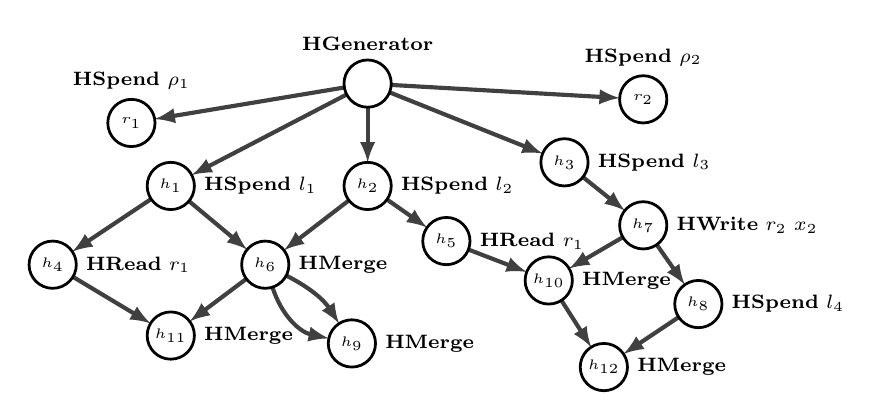
\begin{tikzpicture}
\SetVertexStyle[FillOpacity=0]
\Vertex[label=$\mathbf{HGenerator}$,x=0,y=0,position=above]{H0}
\Vertex[y=-1.3,x=-2.5,label=$\mathbf{HSpend}\ l_1$,position=0]{L1}
\Vertex[y=-1.3,x=0,label=$\mathbf{HSpend}\ l_2$,position=0]{L2}
\Vertex[y=-1,x=2.5,label=$\mathbf{HSpend}\ l_3$,position=0]{L3}
\Vertex[y=-2.3,x=-4,label=$\mathbf{HRead}\ r_1$,position=0]{R1}
\Vertex[y=-2,x=1,label=$\mathbf{HRead}\ r_1$,position=0]{R2}
\Vertex[y=-2.3,x=-1.3,label=$\mathbf{HMerge}$,position=0]{M1}
\Vertex[y=-1.8,x=3.5,label=$\mathbf{HWrite}\ r_2\ x_2$,position=0]{W1}
\Vertex[y=-2.8,x=4.2,label=$\mathbf{HSpend}\ l_4$,position=0]{S4}
\Vertex[y=-3.3,x=-0.2,label=$\mathbf{HMerge}$,position=0]{M2}
\Vertex[y=-3.6,x=3.0,label=$\mathbf{HMerge}$,position=0]{M3}
\Vertex[y=-3.2,x=-2.5,label=$\mathbf{HMerge}$,position=0]{M4}
\Vertex[y=-2.5,x=2.3,label=$\mathbf{HMerge}$,position=0]{M5}
\SetTextStyle[TextFont=\tiny]
\Text[y=-1.3,x=-2.5]{$h_1$}
\Text[y=-1.3,x=0]{$h_2$}
\Text[y=-1,x=2.5]{$h_3$}
\Text[y=-2.3,x=-4]{$h_4$}
\Text[y=-2,x=1]{$h_5$}
\Text[y=-2.3,x=-1.3]{$h_6$}
\Text[y=-1.8,x=3.5]{$h_7$}
\Text[y=-2.8,x=4.2]{$h_8$}
\Text[y=-3.3,x=-0.2]{$h_9$}
\Text[y=-3.6,x=3.0]{$h_{12}$}
\Text[y=-3.2,x=-2.5]{$h_{11}$}
\Text[y=-2.5,x=2.3]{$h_{10}$}
\Edge[Direct](H0)(L1) \Edge[Direct](H0)(L2) \Edge[Direct](H0)(L3)
\Edge[Direct](L1)(R1) \Edge[Direct](L1)(M1) \Edge[Direct](L2)(M1) \Edge[Direct](L3)(W1)
\Edge[Direct,bend=15](M1)(M2) \Edge[Direct,bend=-30](M1)(M2)
\Edge[Direct](W1)(S4) \Edge[Direct](R1)(M4) \Edge[Direct](M1)(M4) \Edge[Direct](S4)(M3)
\Edge[Direct](L2)(R2) \Edge[Direct](W1)(M5) \Edge[Direct](R2)(M5) \Edge[Direct](M5)(M3)

\Vertex[y=-0.5,x=-3.0,label=$\mathbf{HSpend}\ \rho_1$,position=above]{R1}
\Vertex[y=-0.2,x=3.5,label=$\mathbf{HSpend}\ \rho_2$,position=above]{R2}
\Text[y=-0.5,x=-3.0]{$r_1$}
\Text[y=-0.2,x=3.5]{$r_2$}
\Edge[Direct](H0)(R1) \Edge[Direct](H0)(R2)

\end{tikzpicture}
\caption{历史流的示例} \label{fig:His1}
\end{figure}

历史流表述了汇点的所有依赖对系统资源的访问历史,
系统资源的键 ResKey 亦是用历史流表示的,ResKey 的类型亦是 history。
首先历史流足以表达所有的系统资源键,实际上字符串就足以表达所有的系统资源键,
例如“文件:/某个/文件/的/路径”或者“内存:12345678地址”。
%因为所有字符串的数目为
%$\aleph_1$,且对一个程序有意义的系统资源数目是有限的或至多同构于自然数集的无穷,
%而字符串集同构于自然数集同构于历史流集。
另一方面系统资源可能随着程序的进行而产生,如动态分配的内存,用历史流表示资源键的好处是,
在某个历史点$h_1$表示的操作后若产生了一个新的系统资源(比如新分配了某段内存),
其键就可以表示为$\mathbf{HSpend}\ l\ h_1$
,与在别的历史点$h_2$后产生的资源$\mathbf{HSpend}\ l\ h_2$ 区分开,
而资源键的标号可以简单地费用为0地表示 $l=\mathbf{Label}\ "\texttt{{资源标识}"}\ 0$.
图\ref{fig:His1}中的 $r_1$ $r_2$ 是这样的例子。

如果两个历史流执行了完全相同的操作,那么这两个历史流是相等的。
而 $\mathbf{HSpend}$ 除了标记操作的费用还用以区分不同的操作。
例如图\ref{fig:His1}中,$h_4$与$h_5$的对$r_1$的读取发生在不同的操作$h_1$与$h_2$之后,
$h_1$与$h_2$使用不同的标号$l_1$与$l_2$区分开来,若$l_1=l_2$则$h_1=h_2$且$h_4=h_5$。
即两个线程若执行完全相同的操作则这两个线程的历史流亦是相同的,这导致在抽象机中
实际上无法区分这两个线程。这是合理的并且是种优点,
若两个线程执行了完全相同的操作就意味着其数值结果以及每次对系统状态的
修改也相同,那么不需要也没有理由区分这两者。

%非常有趣的一点是,
不同于普通的状态机理论,程序只能在变化的却始终唯一的
一个状态上进行,历史流的世界中存在多条时间线,每一个节点都记录了一个历史
,而节点与节点之间的历史是可以不同的,如 $h_{11}$ 与 $h_{12}$,
进而各自的时间线也不尽相同。例如在 $h_{11}$ 的时间线上$r_2$资源还完好如
初,而$h_{12}$ 上就已经被修改;某个历史流节点的世界中某个文件还可
以被正常读取而另一个历史流节点中该文件可能已被删除。
存在众多的时间线,各个操作只确信其所依赖的那一个历史流节点
,只认同并访问此历史节点所记录的状态;只在此历史上继续发展而
接续新的历史记录。

两条历史线通过合并操作 $\mathbf{HMerge}$ 汇合,合并检验两条历史线的相容,
双方是否进行了互斥的读写。

\begin{defin}[历史流的有效性]
历史流$h$的包括自身在内的所有依赖$\mathbf{HIS\_ANCENSTOR}\ h$
\begin{align*}
&\mathbf{HIS\_ANCENSTOR}\ \mathbf{HGenerator} &&\coloneqq \emptyset \\
    &\mathbf{HIS\_ANCENSTOR}\ (\mathbf{HSpend}\ l\ h) &&\coloneqq 
    (\mathbf{HSpend}\ l\ h)\ \mathbf{INSERT}\ 
    (\mathbf{HIS\_ANCENSTOR}\ h)\\
    &\mathbf{HIS\_ANCENSTOR}\ (\mathbf{HRead}\ r\ h) &&\coloneqq
    (\mathbf{HRead}\ r\ h)\ \mathbf{INSERT}\ 
    (\mathbf{HIS\_ANCENSTOR}\ h)\\
    &\mathbf{HIS\_ANCENSTOR}\ (\mathbf{HWrite}\ r\ x\ h) &&\coloneqq 
    (\mathbf{HWrite}\ r\ x\ h)\ \mathbf{INSERT}\ 
    (\mathbf{HIS\_ANCENSTOR}\ h)
\end{align*}
历史流$h$的种类谓词
\begin{align*}
\begin{split}
    &\mathbf{IS\_READ}\ (\mathbf{HRead}\ r\ h) \coloneqq \T \\
    &\mathbf{IS\_READ}\ \_ \coloneqq \F
\end{split} \begin{split}
    &\mathbf{IS\_WRITE}\ (\mathbf{HWrite}\ r\ x\ h) \coloneqq \T \\
    &\mathbf{IS\_WRITE}\ \_ \coloneqq \F
\end{split}
\end{align*}
式中“\_”表示所有其他构造函数。
历史流$h$的所有写入$\mathbf{HIS\_WRITE}\ h$
    \[ \mathbf{HIS\_WRITE}\ h = (\mathbf{HIS\_ANCENSTOR}\ h) \cap
    (\mathbf{IS\_WRITE}\ h)\]
历史流$h$的所有读取$\mathbf{HIS\_READ}\ h$
    \[ \mathbf{HIS\_READ}\ h = (\mathbf{HIS\_ANCENSTOR}\ h) \cap
    (\mathbf{IS\_READ}\ h)\]
历史流$h$的所有资源访问$\mathbf{HIS\_ACCESS}\ h$
    \[ \mathbf{HIS\_ACCESS}\ h \coloneqq (\mathbf{HIS\_WRITE}\ h) \cup 
    (\mathbf{HIS\_READ}\ h)\]
所有资源访问操作h的目标资源$\mathbf{HIS\_REF}\ h$
\begin{align*}
    &\mathbf{HIS\_REF}\ (\mathbf{HRead}\ r\ h) \coloneqq r
    &\mathbf{HIS\_REF}\ (\mathbf{HWrite}\ r\ x\ h) \coloneqq r
\end{align*}
合并的 CREW 合法性
\begin{multline*}
    \mathbf{CRITICAL\_VALID}\ h_1\ h_2 \coloneqq \\
    \forall h_r\ h_w.\ h_r \in (\mathbf{HIS\_ACCESS}\ h_1) \cup
    (\mathbf{HIS\_ACCESS}\ h_2) \land \\
    h_w \in (\mathbf{HIS\_WRITE}\ h_1) \cup (\mathbf{HIS\_WRITE}\ h)
    \land (\mathbf{HIS\_REF}\ h_r = 
    \mathbf{HIS\_REF}\ h_w) \Rightarrow \\
    (h_w \in \mathbf{HIS\_ANCENSTOR}\ h_r) \lor
    (h_r \in \mathbf{HIS\_ANCENSTOR}\ h_w)
\end{multline*}
即,$h_1$与$h_2$ 中对同一资源的访问与写入不是依赖于一方就是被依赖于一方。

\noindent 历史流$h$的有效性$\mathbf{VALID\_HIS}\ h$
\begin{align*}
    &\mathbf{VALID\_HIS}\ \mathbf{HGenerator} &&\coloneqq \T \\
    &\mathbf{VALID\_HIS}\ (\mathbf{HSpend}\ l\ h) &&\coloneqq \mathbf{VALID\_HIS}\ h \\
    &\mathbf{VALID\_HIS}\ (\mathbf{HWrite}\ r\ x\ h) &&\coloneqq
    \mathbf{VALID\_HIS}\ h\\
    &\mathbf{VALID\_HIS}\ (\mathbf{HRead}\ r\ h) &&\coloneqq \mathbf{VALID\_HIS}\ h\\
    &\mathbf{VALID\_HIS}\ (\mathbf{HMerge}\ h_1\ h_2) &&\coloneqq
    \mathbf{CRITICAL\_VALID}\ h_1\ h_2
\end{align*}
\end{defin}

可以从历史流中还原出状态

\begin{defin}[历史流的状态]
$\mathbf{HIS\_STAT} : \mathrm{history} \rightarrow \mathrm{status}$
其中 $\mathrm{status} \Coloneqq \mathrm{history} \mapsto \mathrm{number}$
是有限映射(finite map)类型。
\begin{align*} 
    &\mathbf{HIS\_STAT}\ \mathbf{HGenerator} &&\coloneqq&& \mathbf{FEmpty} \\
    &\mathbf{HIS\_STAT}\ (\mathbf{HSpend}\ l\ h) &&\coloneqq&&
    \mathbf{HIS\_STAT}\ h \\
    &\mathbf{HIS\_STAT}\ (\mathbf{HRead}\ r\ h) &&\coloneqq&&
    \mathbf{HIS\_STAT}\ h \\
    &\mathbf{HIS\_STAT}\ (\mathbf{HWrite}\ r\ x\ h) &&\coloneqq&&
    (r, x)\ \fupdate\ \mathbf{HIS\_STAT}\ h \\
\end{align*}
\end{defin}

$\mathrm{status} \Coloneqq \mathrm{history} \mapsto \mathrm{number}$,
以自然数表示状态难以分析,可以建立资源状态到自然数的单射,
并同样的资源键到历史流的单射。
例如若有单射 $\mathrm{AccountName} : \mathrm{string} \rightarrow 
\mathrm{history}$,$\mathrm{Deposit} : \mathrm{currency} \rightarrow
\mathrm{number}$,那么某个状态可表示为
\begin{multline}
    (\mathrm{AccountName}\ \textnormal{"Alice"},\ \mathrm{Deposit}\ 
(100\ \mathrm{RMB})) \fupdate \\
(\mathrm{AccountName}\ \textnormal{"Bob"},\ \mathrm{Deposit}\ 
    (200\ \mathrm{USD})) \fupdate \cdots \fupdate \mathbf{FEmpty}
\end{multline}

\begin{defin}[历史流的费用] 历史流同样记录了至今为止的所有开销进而可以
还原至今为止的费用
\begin{align*}
    &\mathbf{HIS\_FEE}\ \mathbf{HGenerator} &&\coloneqq&& 0&\\
    &\mathbf{HIS\_FEE}\ (\mathbf{HSpend}\ l\ h) &&\coloneqq&& 
    \mathbf{LABEL\_FEE}\ l\ +\ \mathbf{HIS\_FEE}\ h&\\
    &\mathbf{HIS\_FEE}\ (\mathbf{HRead}\ r\ h) &&\coloneqq&& 
    \mathbf{HIS\_FEE}\ h&\\
    &\mathbf{HIS\_FEE}\ (\mathbf{HWrite}\ r\ x\ h) &&\coloneqq&& 
    \mathbf{HIS\_FEE}\ h&\\
&\mathbf{LABEL\_FEE}\ (\mathbf{Label}\ name\ fee) &&\coloneqq&&fee&
\end{align*}
而费用的具体定义是框架性的,允许根据实现定制,可以包括时间、空间费用。
\end{defin}

最后历史流是可以自然地纳入{\phew}的,例如

\begin{example}[历史流纳入{\phew}]
    令类型 phenoval 表示原本的{\phew}类型 phenomenon,而定义新的{\phew}
    phenomenon 如下
    \[ \mathrm{phenomenon} \Coloneqq \mathbf{Phenomenon}\ 
    \mathrm{phenoval}\ \mathrm{history} \]
\end{example}

%历史流融入{\phew}的方式并非必须如此,但一定拥有函数
%$\mathbf{P_H}$ 以得到{\phew}中的历史流,
%$\mathbf{P_V}$ 得到{\phew}中的数值部分。
%\begin{align*}
%    &\mathbf{PHE\_VAL}\ (\mathbf{Phenomenon}\ v\ h) \coloneqq v&
%    &\mathbf{P_V} \coloneqq \mathbf{PHE\_VAL} \\
%    &\mathbf{PHE\_HIS}\ (\mathbf{Phenomenon}\ v\ h) \coloneqq h&
%    &\mathbf{P_H} \coloneqq \mathbf{PHE\_HIS}
%\end{align*}

\subsection{依赖}

纯粹数值计算中只有数值依赖,如果对某值的计算不影响对最终结果的计算,
即此值的计算是不被依赖的,就可以完全删除。
%那么对此值的计算是完全不需要的、不被依赖的,故而可以安全地优化掉。

在基于历史流的有状态计算中,操作通过历史流读取状态,
状态转移操作通过在历史流的末尾接续访问标记以修改状态,
状态转移操作能影响后续当且仅当其构造的新历史流被后续操作的历史流包含。
历史是{\phew}的一部分,%历史融入后历史就被改变进而{\phew}也被改变,
后续的{\phew}的历史中包含先前操作的历史,因此后续的{\phew}依赖于先前的状态转移操作。
%于是对状态的修改就会影响之后的{\phew},之后的{\phew}也就依赖于这次状态的修改,
%这操作就不能被减掉。%亦即,
{\phew}中包含历史进而包含状态,状态依赖就成为一种计算依赖。

状态转移操作可以由$\mathbf{Then}$ 运算影响到后续的历史:
\begin{defin}[$\mathbf{Then}$操作]
    \[ \mathbf{Then}\ p_1\ p_2 \coloneqq \mathbf{Phenomenon}\ 
    (\mathbf{P_V}\ p_1)\ (\mathbf{HMerge}\ (\mathbf{P_H}\ p_1)\ 
    (\mathbf{P_H}\ p_2))\]
\end{defin}

即,抛弃$p_2$的结果$(\mathbf{P_V}\ p_2)$ 而只保留$p_1$的,
而合并双方的历史,于是$p_2$对状态的改变可以传递给后续。

在无状态而纯粹数值计算的情形,$\mathbf{Then}$ 操作直接成为
\[ \mathbf{Then}\ p_1\ p_2 = p_1 \]
即 \[ \mathbf{Then} = \K \]
$p_2$ 的一切操作,都会被优化掉而不产生任何后续影响。





	\chapter{用于智能合约的 \Eamlh 的实现}

\section{用于智能合约的抽象机器 \amlhS 在 HOL 上的实现}

首先论述 HOL 交互式定理证明器上用于智能合约的抽象机器 \amlhS 的实现,
这一实现通过 HOL 定理证明器上4867行的 SML 语言完成。
状态方面采用计算与状态分离的方案,将所有状态转移以指令的方式记录而在
智能合约所有计算完成后的最后写入区块链,这样更安全。

\begin{defin}[现象的定义] 类型 phenomenon 表示现象
\[ \begin{split}
\mathrm{phenomenon} \Coloneqq & \PhV\ \mathrm{num}\ 
\mathrm{num} \mbar \PhS\ \mathrm{phenomenon}\ 
\mathrm{phenomenon} \\
\mbar & \PhP \mathrm{phenomenon}
\end{split} \]
$\PhV x\ b$ 表示 $b$ 个二进制表示的数字 $x$。$\PhS p_1\ p_2$ 表示两个值
在内存上的直接拼接构成的现象。$\PhP p$ 表示对现象 $p$ 的指针。
\[ \begin{array}{lcllcl}
\PB\ (\PhV x\ b) &\coloneqq& b&
\PX\ (\PhV x\ b) &\coloneqq& x\\
\PB\ (\PhS p_1\ p_2) &\coloneqq& \PB p_1 + \PB p_2\quad\quad&
\PX\ (\PhS p_1\ p_2) &\coloneqq& \PX(p_1) + \PX(p_2) \cdot 2^{\PB(p_1)}\\
\PB\ (\PhP p) &\coloneqq& \mathrm{PointerSize} &&&
\end{array} \]
$\PX\ (\PhP p)$ 故意的不去定义。PointerSize 为常量固定为智能合约执行环境
的位数,一般为32。
现象的分割工具,函数 $\PL,\ \PU$
    \begin{align*} \PL n\ p &= \PhV\ (\PX p \Mod 2^n)\ n&
        \PU n\ p &= \PhV\ (\PX p \Div 2^n)\ (\PB p \dotminus n)&
    \end{align*}
合法的现象
\begin{gather*} \begin{align*}
\VP\ (\PhV\ x\ b) &\coloneqq (x < 2^b)&
\VP\ (\PhP\ p) &\coloneqq \VP p&
\end{align*}\\
\VP\ (\PhS\ p_1\ p_2) \coloneqq \VP p_1 \ \land\ \VP p_2
\end{gather*}
现象集的 0 元素是 $\mathbf{PhV}\ 0\ 0$,
占用0个比特位的值,且其是合法的。
\end{defin}

\begin{defin}[\amlhS 上的理解]
\amlhS 上理解的定义基本基于定义 \ref{Def.itp} ,只是固定了理解的现象集
的位数目。
    \[ \begin{split}
        \itp{\alpha} \Coloneqq \mathbf{Noesis}\ &(\alpha \rightarrow \phenomenon)
        \ (\phenomenon \rightarrow \alpha)\\
    &(\alpha\ \mathrm{set})\ (\phenomenon\ \mathrm{set})\ \mathrm{num}
    \end{split} \]
\begin{gather*}
\begin{align*}
\mathbf{NOE\_LIGHT}\ (\mathbf{Noesis}\ l\ tr\ s_e\ s_p\ s) & = l&
\mathbf{NOE\_TRANSCEND}\ (\mathbf{Noesis}\ l\ tr\ s_e\ s_p\ s) & = tr&\\
\mathbf{NOE\_SET}\ (\mathbf{Noesis}\ l\ tr\ s_e\ s_p\ s) & = s_e&
\mathbf{NOE\_SIZE}\ (\mathbf{Noesis}\ l\ tr\ s_e\ s_p\ s) &= s&
\end{align*}\\
\mathbf{NOE\_PSET}\ (\mathbf{Noesis}\ l\ tr\ s_e\ s_p\ s)
 = s_p \cap \{ p \mbar \PB p = s \}
 \end{gather*}
同样有记号
\begin{gather*}
\begin{align*}
    \mathbf{Li}_i\ & \coloneqq \mathbf{NOE\_LIGHT}\ i&
    \mathbf{Tr}_i\ & \coloneqq \mathbf{NOE\_TRANSCEND}\ i &
\end{align*}\\ \begin{align*}
    \mathbf{Sp}_i\ & \coloneqq \mathbf{NOE\_PSET}\ i&
    \mathbf{Si}_i\ & \coloneqq \mathbf{NOE\_SIZE}\ i&
    \mathbf{Se}_i\ & \coloneqq \mathbf{NOE\_SET}\ i&
\end{align*} \end{gather*}
$\mathbf{Si}_i$ 表示理解 $i$ 的现象集的比特数。
\end{defin}

\begin{defin}[\amlhS 的 Noesis 对应] 在定义 \ref{Def.TR} 的基础上
加入现象合法性。
\[ p \widesim{i} e \coloneqq \mathbf{V}_i\ \land\ \VP\ p\ \land\ 
p \in \mathbf{Sp}_i\ \land\ (\mathbf{Tr}_i\ p = e) \]
\end{defin}

其余理论均与第 \ref{Ch.AmLH} 章相同。

\begin{defin}[链的抽象表达]
\amlhS 将链上数据抽象为各个由标识区分的键值表,使用有限映射表示,
类型 chain 为此别名 
\[ \mathrm{chain} \Coloneqq (\mathrm{string},\ \mathrm{phenomenon})
\mapsto \mathrm{phenomenon} \]
类型 write\_chain 表示对链的写入操作命令,也是一个别名
\[ \mathrm{write\_chain} \Coloneqq ((\mathrm{string},\ 
\mathrm{phenomenon}),\ \mathrm{phenomenon}) \]
元组 $((name,\ key),\ value)$ 表示以值 $value$ 写入到表 $name$ 的
键 $key$ 的写入操作。
有限映射的更新操作 $\fupdate$ 就表示对链数据的写入。
\end{defin}

链数据写入命令的内存结构为
\begin{center}
\begin{tabular}{|c|c|c|c|c|} \hline
\text{表标识}&\text{键指针}&
\text{键大小}&\text{值指针}&\text{值大小}\\
\text{8bits}&\text{PointerSize} bits&
\text{32bits}&\text{PointerByte} bits&\text{32bits} \\ \hline
\end{tabular}
\end{center}
表标识占用1字节,理论上表标识可以是任意字符串,但在最终的编译实现中,
一段合约所有使用的表标识会被唯一地分配$0\sim255$的编号,使用此编号表示
表标识,故一个合约支持访问的表数量不超过256个。

\begin{defin}[智能合约调用响应]
类型 response 表示所期望的智能合约调用的返回类型。
\[ \combtyp{response}{\alpha} \Coloneqq \Rsp \alpha\ (\combtyp{list}{
    \mathrm{write\_chain}}) \]
$\Rsp\ x\ l$ 表示以 $x$ 为返回值,$l$ 为链数据写入命令序列的智能合约调用
响应。$l$ 列表中的每一项元素都是 write\_chain 类型描述的链数据的写入命令
。一个智能合约的作为外部接口的函数必须返回 response 类型,编译时会在
每个外部接口函数的实现的最后逐一遍历写入命令序列 $l$,逐一将命令执行并
写入进链中。智能合约调用响应在实现上的内存结构是
\begin{center}
\begin{tabular}{|c|c|} \hline
\text{指向写入命令序列 $l$ 的指针}&\text{计算结果 $x$}\\
\text{PointerSize bits}&\text{$\mathbf{Si}_i$ bits}\\ \hline
\end{tabular}
\end{center}
\end{defin}

\amlhS 所有定义的理解列于表 \ref{tab.IC.noesis} 与表 
 \ref{tab.IC.noesis2} 中。所有的基元指令及其定义与 Noesis 同构列于
表 \ref{tab.IC.primop} 与表 \ref{tab.IC.primop2} 中。

\begin{table}
\begin{threeparttable}
\centering \caption{\amlhS 中实现的理解} \label{tab.IC.noesis}
\begin{tabular}{ |c|c|c|c|p{4.5cm}|p{2cm}| } \hline
\textbf{理解} & \textbf{本体集} & \textbf{现象集} & 
$\mathbf{Si}$ \textbf{值} & $\mathbf{Li}$ \textbf{映射} & 
$\mathbf{Tr}$ \textbf{映射} \\ \hline
$\NatSegI\ n$ & $\{x\mbar x < n\}$ & $\mathbb{U}_\mathrm{pv}$ & $n$
& $\lambda e.\ \PhV e\ \lceil \log_2\ n \rceil$ & $\PX$ 
\\ \hline
$\BoolI$ & $\univ{bool}$ & $\mathbb{U}_\mathrm{pv}$ & $1$ &
$\lambda e.\ \PhV\ ($\newline$\xif\ e\ \xthen\ 1\ \xelse\ 0)\ 1$&
$\lambda v.$ \newline $\PX v > 0$  \\ \hline 
$\AddressI$ & $\{ n \mbar n < \mathrm{AdrSize} \}$ &
$\mathbb{U}_\mathrm{pv}$ & AdrBits & $\lambda e.\ \PhV
e\ \mathrm{AdrBits}$ & $\PX$ \\ \hline
$\OneI\ s$ & $\{ s \}$ & $\mathbb{U}_\mathrm{pv}$ & 0 & 
$\K(\PhV 0\ 0)$ & $\K s$ \\ \hline
$\ListI\ i$ & $\mathrm{EVERY}\ \mathbf{Se}_i$ & 虚构 & Ps & 虚构 
& 虚构 \\ \hline
$\CWI$ & $(\mathbb{U}_\mathrm{str} \times \mathbb{U}_\mathrm{ph}) \times
\mathbb{U}_\mathrm{ph}$ & 虚构 & $8 + 2 \mathrm{Ps}$ & 虚构 
& 虚构 \\ \hline
$\RsI\ i$ & $\{\Rsp\ x\ l \mbar x \in \mathbf{Se}_i\}$ & 虚构 & 
$\mathrm{Ps} + \mathbf{Si}_i$ & 虚构 
& 虚构 \\ \hline
$i \times j$ & $\mathbf{Se}_i \times \mathbf{Se}_j$ & 
见注1 & $\Si_i + \Si_j$ & $\lambda(x,y).\ \PhS\ \Li_i(x)\ 
\Li_j(x)$ & 见注2 \\ \hline
\end{tabular}
\begin{tablenotes} \small 
\item $\mathbb{U}_\mathrm{pv}$ 是 $\{ \PhV x\ b \}$ 的简写,
表示现象类型的所有元素中由 $\PhV$ 构造的。
$\mathbb{U}_\mathrm{ph}$ 是 $\univ{phenomenon}$ 的简写,
表示现象类型中所有的元素。
$\mathbb{U}_\mathrm{str}$ 是 $\univ{string}$ 的简写。
$\mathrm{Ps}$ 是 PointerSize 的简写。
 EVERY 是 HOL 系统库中的函数,$\mathrm{EVERY}\ s$ 
表示所有元素都属于 $s$ 集的所有列表构成的集合。
\item[注1] 理解 $i \times j$ 的现象集是 $\{\PhS p_1\ p_2
\mbar p_1\in \Sp_i\land p_2 \in \Sp_j\}$,表格空间有限故列于此。
\item[注2] 理解 $i \times j$ 的\textbf{Tr}映射是 
    $\lambda p.\ (\Tr_i(\PL\ \Si_i\ p),\ \Tr_j(\PU\ \Si_i\ p))$,
    表格空间有限故列于此。
\end{tablenotes}
\end{threeparttable}
\newline \newline
\begin{threeparttable}
\centering \caption{\amlhS 中实现的理解(绪)} \label{tab.IC.noesis2}
\begin{tabular}{ |c|p{14.8cm}| } \hline
\textbf{理解} & \textbf{描述} \\ \hline
$\NatSegI\ n$ & 不超过 $n$ 的自然数 \\ \hline
$\BoolI$ & bool 值 \\ \hline $\AddressI$ & 
智能合约场景下的账户标识,在以太坊中是 \texttt{address} 类型,
EOS.IO 中是 \texttt{name} 类型,常量 AdrSize 表示标识的大小,AdrBits
表示标识的比特数 \\ \hline
$\OneI\ s$ & 单元素集合 $\{s\}$ 的理解,用于表示
状态输入$\{ s \}$ \\ \hline
$\ListI\ i$ & 对元素使用 $i$ 理解的列表理解,虚构定义而来,
在内存中的表示是一个指针,故有 PointerSize 的大小 \\ \hline
$\CWI$ & 是链数据的写入命令的理解,虚构定义而来 \\ \hline
$\RsI\ i$ & 表示以 $i$ 理解为返回内容的智能合约调用响应 \\ \hline
\end{tabular}\end{threeparttable}\end{table}

\begin{table}\begin{threeparttable}
\centering \caption{\amlhS 中基元函数的 Noesis 同构}
\label{tab.IC.primop} \begin{tabular}{ |c|p{5cm}|p{8.1cm}| } \hline
\textbf{基元函数} & \textbf{ Noesis 同构 } & \textbf{描述} \\ \hline
$\mathbf{IAdd}\ n$ & $\mathbf{IAdd}\ n \proctr{\NatSegI n|\NatSegI n|
\NatSegI n}{\lambda x\ y.\ x + y < 2^n} (+) $ &
$n$ 位整数加法的自然数加法对应 \\ \hline
$\mathbf{ISub}\ n$ & $\mathbf{ISub}\ n \proctr{\NatSegI n|\NatSegI n|
\NatSegI n}{\lambda x\ y.\ x \geq y} (-)$ & $n$ 位整数减法的自然数减法
对应 \\ \hline
$\mathbf{IMul}\ n$ & $\mathbf{IMul}\ n \proctr{\NatSegI n|\NatSegI n|
\NatSegI n}{\lambda x\ y.\ x * y < 2^n} (\times)$ & $n$ 位整数乘法
的自然数乘法对应 \\ \hline
$\mathbf{ILt}\ n$ & $\mathbf{ILt}\ n \proctr{\NatSegI n|\NatSegI n|
\BoolI}{\lambda x\ y.\ \T} (<)$ & $n$ 位整数小于判断的自然数小于对应 
\\ \hline
$\mathbf{ILe}\ n$ & $\mathbf{ILe}\ n \proctr{\NatSegI n|\NatSegI n|
\BoolI}{\lambda x\ y.\ \T} (\leq)$ & $n$ 位整数小于等于的自然数小于等于对应 \\ \hline
$\mathbf{IEq}\ n$ & $\mathbf{IEq}\ n \proctr{\NatSegI n|\NatSegI n|
\BoolI}{\lambda x\ y.\ \T} (=)$ & $n$ 位整数等于判断的自然数等于对应 \\ \hline
$\mathbf{IEq}\ \mathrm{AdrBits}$ & $\mathbf{IEq}\ \mathrm{AdrBits}
\proctr{\AddressI|\AddressI|\BoolI}{\lambda x\ y.\ \T} (=)$ & 
$n$ 位整数等于判断的账户标识对应 \\ \hline
$\mathbf{INot}$ & $\mathbf{INot} \proctr{\BoolI|\BoolI}
{\lambda x.\ \T} (\lnot)$ & bool 值取反 \\ \hline
$\mathbf{Append}\ i$ & $\mathbf{Append}\ i \proctr{i|\ListI\ i|\ListI\ 
i}{\lambda l\ x.\ \T} (::)$ & 增加元素到列表的末尾,$(::)$
是 HOL 系统库中列表的增加函数,$1::[2]$ 表示 $[1,2]$ \\ \hline
$\mathbf{Write}\ c\ i\ j$ & $\mathbf{Write}\ c\ i\ j 
\proctr{i|j|\CWI}{\lambda k\ v.\ \T}$\newline$
(\lambda k\ v.\ ((c,\ \mathbf{Li}_i\ k),\ \mathbf{Li}_j\ v))$ &
写入链数据的表$c$的键$k$为$v$的操作,产生写入命令 \\ \hline
$\mathbf{Read}\ c\ x\ i\ j$ & $\mathbf{Read}\ c\ x\ i\ j 
\proctr{\OneI\ x|i|j}{\lambda k.\ (c,k) \in \Dom x}$\newline$
(\lambda k.\ x\ (c,k))$ &
对给定的链数据 $x$,表标识 $c$,读取链数据$x$的表$c$的$k$键 \\ \hline
$\mathbf{Cart}$ & $\mathbf{Cart} \proctr{i|j|i\times j}{\lambda k.\ (c,k) \in \Dom x}$\newline$
(\lambda k.\ x\ (c,k))$ &
对给定的链数据 $x$,表标识 $c$,读取链数据$x$的表$c$的$k$键 \\ \hline
\end{tabular} \end{threeparttable} 
\newline \newline
\begin{threeparttable}%
\centering \caption{\amlhS 中基元函数的定义} \label{tab.IC.primop2}
\begin{tabular}{ |c|p{13.6cm}| } \hline
\textbf{基元函数} & \textbf{定义} \\ \hline
$\mathbf{IAdd}\ n$ & $\PB p_1 = \PB p_2 = n \Rightarrow
\mathbf{IAdd}\ n\ p_1\ p_2 \coloneqq
\PhV\ (\PX p_1 + \PX p_2 \mod 2^n)\ n$ \\ \hline
$\mathbf{ISub}\ n$ & $\PB p_1 = \PB p_2 = n \Rightarrow
\mathbf{ISub}\ n\ p_1\ p_2 \coloneqq
\PhV\ (\PX p_1 - \PX p_2 \mod 2^n)\ n$ \\ \hline
$\mathbf{IMul}\ n$ & $\PB p_1 = \PB p_2 = n \Rightarrow
\mathbf{IMul}\ n\ p_1\ p_2 \coloneqq
\PhV\ (\PX p_1 * \PX p_2 \mod 2^n)\ n$ \\ \hline
$\mathbf{ILt}\ n$ & $\PB p_1 = \PB p_2 = n \Rightarrow
\mathbf{ILt}\ n\ p_1\ p_2 \coloneqq
\PhV\ (\xif \PX p_1 < \PX p_2 \xthen 1 \xelse 0)\ n$ \\ \hline
$\mathbf{ILe}\ n$ & $\PB p_1 = \PB p_2 = n \Rightarrow
\mathbf{ILe}\ n\ p_1\ p_2 \coloneqq
\PhV\ (\xif \PX p_1 \leq \PX p_2 \xthen 1 \xelse 0)\ n$ \\ \hline
$\mathbf{IEq}\ n$ & $\PB p_1 = \PB p_2 = n \Rightarrow
\mathbf{IEq}\ n\ p_1\ p_2 \coloneqq
\PhV\ (\xif \PX p_1 = \PX p_2 \xthen 1 \xelse 0)\ n$ \\ \hline
$\mathbf{INot}$ & $ \PB p = 1 \Rightarrow
\mathbf{INot}\ p = \PhV\ (\xif \PX p = 0 \xthen 1 \xelse 0)\ 1$\\ \hline
$\mathbf{Append}\ i$ & 虚构定义自同构
$\mathbf{Append}\ i \proctr{i|\ListI\ i|\ListI\ 
i}{\lambda l\ x.\ \T} (::)$ \\ \hline
$\mathbf{Write}\ c\ i\ j$ & 虚构定义自同构 $\mathbf{Write}\ c\ i\ j 
\proctr{i|j|\CWI}{\lambda k\ v.\ \T}
(\lambda k\ v.\ ((c,\ \mathbf{Li}_i\ k),\ \mathbf{Li}_j\ v))$ \\ \hline
$\mathbf{Read}\ c\ x\ i\ j$ & 虚构定义自同构 $\mathbf{Read}\ c\ x\ i\ j 
\proctr{\OneI\ x|i|j}{\lambda k.\ (c,k) \in \Dom x}
(\lambda k.\ x\ (c,k))$ \\ \hline
$\mathbf{Cart}$ & $\mathbf{Cart}\ p_1\ p_2 \coloneqq \PhS p_1\ p_2$ \\ \hline
\end{tabular}\end{threeparttable}\end{table}


\begin{defin}[智能合约的外部接口]
所有 \amlhS 的智能合约所暴露的可供外部调用的接口应是一种现象函数,
且其具有至少一种 Noesis 同构,此同构满足第一个参数的理解必为 
$\OneI\ (x:\mathrm{chain})$,且返回值的理解必为 $\RsI\ k$。即
函数 $f$ 应满足如下形式的 Noesis 同构
\[ f \proctr{\OneI\ x|\cdots|\RsI\ k}{cond} \phi \]
\end{defin}



	\chapter{结论与比较}

{\it 演绎定理以构建程序,}

这不是本文的原创,而仅仅是 Curry-Howard 同构所蕴含的小小推论。
Coq 系列很早就意识到了这点,并围绕此发展出程序式的证明方式
(\textit{proof as program})。
但 Coq 仅仅将定理的演绎与程序的构建限定在直觉主义类型与 λ 演算。
λ 演算非常优秀也能表达几乎所有的计算逻辑,以至于人们都忽略了
类型关系那小小的冒号。

既然是,{\it 演绎定理以构造程序},定理就根本不只限于类型定理也自然不限于
类型的二元关系。本文最梦幻的贡献在于找到了类型关系的一种扩展,Noesis
对应,以及相应由类型系统扩展而来的 Noesis 系统,并演绎 Noesis 对应与
同构的定理以构建程序的开发方法。

\section{与依赖类型系统的比较}

Coq 与基于依赖类型的编程语言如 Agda,Idris,它们非常优秀,但始终处于
理论证明工具与程序开发工具的暧昧不清之间。于其上开发的程序,必须同时
兼顾作为证明的理论上的简谐,与作为程序的工程实践的性能。
程序构造必须数学的同时又工程。这意味着既要把本应用于工程的程序代码
拿去做数学证明,又不能丢失作为程序的本质,必须要考虑性能与实现;
又要把本应描述数学性质的作为类型的定理拿去描述工程,还不能丢失理论
简谐性。无论哪一者都带来很多麻烦,于是这种暧昧的结果是同时损害了
工程实现的性能与用户证明的性能,特别是
工程实现的性能还要额外受制于函数式语言本身的局限。

一个典型的案例是皮亚诺加法用于工程实现的窘境。
皮亚诺数作为普遍的自然数的定义
\[ \mathbb{N} \Coloneqq 0\mbar \Suc \mathbb{N} \]
其上的加法被递归定义
\[ \begin{array}{rcl} 
n + 0 &=& n \\
n + (\Suc m) &=& (\Suc n) + m
\end{array}\]
照此递归定义直接在工程上实现显然很荒谬,对一个简单的自然数 $N$ 的加法
需要消耗$O(N)$ 的复杂度。MCMQ 的方案是将所有系统库中的自然数运算
替换为指令集上的运算或是其他标准库中或者是自己实现的 C 语言函数。
暂且不苛刻地责备这种简单干脆的替换直接割断了 Coq 对一切自然数相关的
理论证明——C 语言上的函数与 Coq 中的自然数理论是两个事物——
而抛开了正确性不管,事实上 MCMQ 对于 C 语言整数运算溢出的处理很值得
怀疑,Coq 的世界中自然数根本没有运算溢出于是一切 MCMQ 编译出的
程序的数值溢出问题只能依靠 MCMQ 开发者的谨慎与认真,
而数值溢出是形式化验证的基础
问题。这些都不是关键的都不去苛刻地指责,关键在于当一个用户遇到了这样
的需求尝试类似实现一个不同的自然数,一些别的有别于系统库的构造时,
他会可怕地发现递归定义无法绕过而编译而得的程序不得不消耗大量的实践。

这种尴尬的构造存在,且很普遍,就是传统编程语言中大量使用的比特位标记
(bit flags)。Coq、Agda、Idris 的思想是无法将几个比特位标记压入小小的
整型中,因为比特位标记的构造对应于数学上的有限集,而这些语言依赖的
重现规则(rewrite rule)不允许位压缩。于是 Coq、Agda、Idris 可能永远
无法顺利地实现一个 IPv4 协议栈程序,除非非常艰难地绕路。

绕路可以让一些问题解决,但工程程序与数理证明之间暧昧的纠缠不清无法剪断。
如果类型关系的冒号太小了又承载了太多,就把它拉长,变成三元关系,右边也
不是定理了而是程序在抽象领域的对应,就像 Noesis 对应关系那样,把
具象的程序与抽象的数理世界划分清晰,而严谨地保持两者的映射关系,显示地
列在形式系统中而不留隐晦。本文的思路,以 Noesis 系统替代类型系统,
并可以同样地像 Coq 那样演绎定理以构造程序似乎很可行。

另一方面,同样的隐晦出现在以类型对程序性质的证明。
类型是一个集合,一些有某种共性的
元素构成的集合而类型反映了这种共性。既然是共性,就必定只是类型中
各个实例的所有特性的一小部分,而人们却期望用类型体现尽可能多的性质。
类型承载的信息对于某个实例全部的特性必然是粗糙的,类型却被期望尽可能
精细。唯一的特例是类型中只包括一个元素,此时类型的性质完全涵盖了所有元素
的所有特性,是精细的极致,但此时类型也失去了泛用性,自然不应被叫做类型。
值得反思类型对于编程语言本应的意义,是否强加给了类型不适合的角色,
而强加的结果,是用户实际证明时的苦难。

本文的 Noesis 系统中,理解承载共性的部分,并在 \amlhS 中理解决定了
函数参数的位宽。理解承载的共性是通用程序与通用函数的通用性所必须的。
而本体承载每一个现象在某个理解下所有的性质,特别是理解的共性之外的特性,
在一个理解下每个本质不同的现象都对应到不同的一个本体,
此理解下的任何特性不会丢失,以允许之后对本体进行任何的分析。
相比而言,对类型的分析始终只能是共性的分析,因为特性全部丢失了;
而若尝试让类型更加精细,就产生了上一段的尴尬局面。



本文期望本文完成了本文的期望,一种廉价而有效可行的开发正确性被证明的
程序实现的方法。它代价不高, 不消耗大量的开发成本, 只需要
专业的数学知识与机器证明技能, 而本身施行起来不复杂不困难, 
进而能被普遍地应用在现实的普通工业生产中;
但却能有效而彻底地证明程序实现的正确性。本文期望 \amlh 是这样的方法,
但最终只有实践能下此定论。

本文的方法已经开始积极地实践,所有的工具链都已完成并开始以工程的检验。
这些实现包括 4867 行的 HOL 交互式证明系统上的 SML 语言,与 9907 编辑壳层
与外部编译器以及测试代码的 Crystal 语言。
总共 433 次版本仓库的提交与 33 个分支中,共计
增删代码 $2\,780\,207$ 行次,包括 $1\,400\,834$ 行的添加与 $1\,379\,373$
行的删除,在各个分支中最后留存总计 $21\,461$ 行。分支与分支间有大量共享
代码故总代码行数不等于分支数乘以单个分支留存的代码行数。图 
\ref{fig:works} 列出了这些数据的统计方法。

\begin{figure}[p]
\caption{本工作的数据统计} \label{fig:works}
\begin{minted}{console}
# 主分支的代码量
$ cloc src --vcs=git
     134 text files.
     134 unique files.                                          
       6 files ignored.
----------------------------------------------------------------------
Language            files          blank        comment           code
----------------------------------------------------------------------
Crystal                69           1194            499           9413
Standard ML            63            575            721           4867
Markdown                1              7              0             18
----------------------------------------------------------------------
SUM:                  133           1776           1220          14298
----------------------------------------------------------------------
# 总提交数
$ git rev-list --all --count
433
# 总分支数
$ git branch | wc -l                    
33
# 总修改量
$ git log  --pretty=tformat: --numstat \
| gawk '{ add += $1; subs += $2; loc += $1 - $2 } END \
{ printf "added lines: %s removed lines: %s total lines: %s\n",\
add, subs, loc }' -
added lines: 1400834 removed lines: 1379373 total lines: 21461
\end{minted}
\end{figure}

\section{与现有形式化方法的比较}

第 \ref{Sec.formal_method} 节已经介绍了三类流行的形式化方法,本节
将一一比较。

第一类 model checker 式的,因为有限的表达能力与证明能力不在讨论范围中。

第二类尝试将程序翻译到另一个证明系统中并以此证明的,它们的缺陷已经在 
\ref{Sec.formal_method} 节论述过了。困难的证明与可疑的翻译正确性。

必须讨论的是著名的 K Framework。

第三类基于依赖系统的,它们非常优秀,本文将一一讨论。



  \appendix
  \chapter{λ 演算介绍} \label{Ch.lambda}

Sørensen 在其讲义中对$\lambda$演算的形式定义非常简洁,
本节直接从 $\lamst$ 开始介绍,朴素 $\lambda$ 演算请参见其讲义第一章,
 $\lamst$参考自讲义第三章,$\lambda2$参考自讲义第十三章
\cite{sorensen2006lecturesC1}。

\section{λ→}

λ→ 演算有两种样式,Curry 式和 Church 式的,本文延续 Sørensen 的提法,
简单地说 Curry 式的λ→演算为λ→演算,而说Church式的为Church式λ→演算。
这两种样式的λ→ 演算本质是相同的,Sørensen 在其讲义中对此有论述,
本文不再赘述。

\begin{defin}[$\lamst$演算] \label{Def.slam}
\begin{enumerate}
\item $V$为无穷的字母表,表示符号。

\begin{equation}
V = \{v_0,v_1,\cdots\}
\end{equation}

\item 字符串集合 $L$ 是无类型 $\lambda$ 演算上的表达式($\lambda$ term),由如下语法定义。
\begin{equation}
L = \bnf{V\ |\ (L\ L)\ |\ (\lambda V \ L)}
\end{equation}

简写 $\underline{(\ \lambda\ x_1\ (\ \lambda\ x_2\ \cdots\ (\ 
    \lambda\ x_n\ y\ )\ \cdots\ )\ )}$ 为
    $\lambda x_1\ x_2\ \cdots\ x_n.\ y$

\item 集合$U$是另一个无穷的字母表,表示类型变量集(type variables)。
\begin{equation}
U = \{\alpha,\beta,\cdots\} 
\end{equation}

\item 字符串集合 $\Pi$ 表示简单类型。
\begin{equation} \label{Pi}
    \Pi = \bnf{U\ |\ (\Pi \rightarrow \Pi)}
\end{equation}

\item 集合 $C$ 表示上下文,是由语法$V : \Pi$定义的字符串集合的幂集。
\begin{equation}
    C = \powerset \bnf{V:\Pi}
\end{equation}
即$C$ 是所有具有如下形式的集合。
        \[ \{x_1:\tau_1, \cdots, x_n : \tau_n\} \]
其中 $x_1,\cdots,x_n \in V$,$\tau_1,\cdots,\tau_n \in \Pi$。

\item 定义上下文$\Gamma = \{x_1:\tau_1,\cdots,x_n:\tau_n\}$ 的符号域 $\mathrm{dom}$
\[ \mathrm{dom}(\Gamma) = \{x_1,\cdots,x_n\}\]
将$\Gamma_1 \cup \Gamma_2$ 写作 $\Gamma_1, \Gamma_2$ 当
        $\mathrm{dom}(\Gamma_1) \cap \mathrm{dom}(\Gamma_2)$ 时。


%\item 定义上下文$\Gamma = \{x_1:\tau_1,\cdots,x_n:\tau_n\}$ 的类型域 $\rvert \Gamma \lvert$
%
%\[ \lvert \Gamma \rvert = \{\tau_1,\cdots,\tau_n\}\]
%
\item $\mathcal{L} = \bnf{L : \Pi}$ 是λ→表达式,
由如下规则定义$C \times \mathcal{L}$ 上的二元关系 $\vdash$

\hfill

\begin{minipage}[b]{0.5\linewidth}
\begin{prooftree}
\AxiomC{$\ $} \RightLabel{(公理)}
\UnaryInfC{$\Gamma, x : \tau \vdash x : \tau$}
\end{prooftree}
\end{minipage}%
\begin{minipage}[b]{0.4\linewidth}
\begin{prooftree}
\AxiomC{$\Gamma, x : \sigma \vdash M : \tau$} \RightLabel{(抽象律)}
\UnaryInfC{$\Gamma \vdash \lambda x. M : \sigma \rightarrow \tau$}
\end{prooftree}
\end{minipage}

\hfill

\begin{minipage}[b]{0.5\linewidth}
\begin{prooftree}
\AxiomC{$\Gamma \vdash M : \sigma \rightarrow \tau$}
\AxiomC{$\Gamma \vdash N : \sigma$} \RightLabel{(组合律)}
\BinaryInfC{$\Gamma \vdash M N : \tau$}
\end{prooftree}
\end{minipage}\begin{minipage}[b]{0.5\linewidth}
\begin{prooftree}
\AxiomC{$\Gamma \vdash (\lambda v\ M)\ x : \tau$}
\RightLabel{($\beta$规约)}
\UnaryInfC{$\Gamma \vdash M[v/x] : \tau$}
\end{prooftree}
\end{minipage}

\hfill

\end{enumerate}

简单类型$\lambda$演算$\lamst$就是三元组 $(L, \Pi, \vdash)$
\end{defin}


\section{Church式λ→}

Church式λ→ 与 Curry 式 λ→ 的主要区别是,Church 式的抽象中的变量需要
显示地标记类型。即Curry式的抽象写作
\[ \lambda x.\ x : \sigma \rightarrow \sigma \]
而 Church 式的写作
\[ \lambda x{:}\sigma.\ x : \sigma \rightarrow \sigma \]

\begin{defin}[Church式λ→]
\begin{gather}
V_C = \bnf{V:\Pi} \\
L_C = \bnf{V \mbar (L\ L) \mbar (\lambda V_C\ L)} \\
\mathcal{L}_C = \bnf{L_C : \Pi}
\end{gather}
定义 $C \times \mathcal{L}_C$ 上的关系 $\vdash$

\begin{minipage}[b]{0.5\linewidth}
\begin{prooftree}
\AxiomC{$\ $} \RightLabel{(公理)}
\UnaryInfC{$\Gamma, x : \tau \vdash x : \tau$}
\end{prooftree}
\end{minipage}%
\begin{minipage}[b]{0.4\linewidth}
\begin{prooftree}
\AxiomC{$\Gamma, x : \sigma \vdash M : \tau$} \RightLabel{(抽象律)}
\UnaryInfC{$\Gamma \vdash \lambda x{:}\sigma. M : \sigma \rightarrow \tau$}
\end{prooftree}
\end{minipage}

\begin{prooftree}
\AxiomC{$\Gamma \vdash M : \sigma \rightarrow \tau$}
\AxiomC{$\Gamma \vdash N : \sigma$} \RightLabel{(组合律)}
\BinaryInfC{$\Gamma \vdash M N : \tau$}
\end{prooftree}

Church 式$\lamst$就是三元组 $(L_C, \Pi, \vdash)$
\end{defin}

\section{λ2}

现在介绍λ2 演算,它有很多名字,System F,二阶λ演算,Girard–Reynolds
多态λ演算。
λ2 演算基于Church式λ→演算论述。

\begin{defin}[λ2]
\[ L_* = \bnf{L \mbar \Lambda\ U\ L_*} \]
并类似地记号 $\Lambda t_1\ t_2\ \cdots\ t_n.\ b$ 表示
    $\underline{\Lambda\ t_1\ \Lambda\ t_2\ \cdots\ \Lambda\ t_n\ b}$,
\[ \Pi_* = \bnf{\Pi \mbar \forall\ U\ \Pi_*} \]
记号 $\forall \tau_1\ \tau_2\ \cdots\ \tau_n.\ b$ 表示
$\underline{\forall\ \tau_1\ \forall\ \tau_2\ \cdots\ \forall\
    \tau_n\ b}$
\[ C_* = \powerset \bnf{V:\Pi \mbar U:*} \]
$\mathcal{L}_* = \bnf{L_* : \Pi_*}$ 是λ2表达式,
定义 $C_* \times \mathcal{L}_*$上的关系 $\vdash$

\hfill

\begin{minipage}[b]{0.5\linewidth}
\begin{prooftree}
\AxiomC{$\ $} \RightLabel{(公理)}
\UnaryInfC{$\Gamma, x : \tau \vdash x : \tau$}
\end{prooftree}
\end{minipage}%
\begin{minipage}[b]{0.4\linewidth}
\begin{prooftree}
\AxiomC{$\Gamma, x : \sigma \vdash M : \tau$} \RightLabel{(抽象律)}
\UnaryInfC{$\Gamma \vdash \lambda x{:}\sigma. M : \sigma \rightarrow \tau$}
\end{prooftree}
\end{minipage}

\begin{prooftree}
\AxiomC{$\Gamma \vdash M : \sigma \rightarrow \tau$}
\AxiomC{$\Gamma \vdash N : \sigma$} \RightLabel{(组合律)}
\BinaryInfC{$\Gamma \vdash M N : \tau$}
\end{prooftree}

\begin{minipage}[b]{0.5\linewidth}
\begin{prooftree}
\AxiomC{$\Gamma,\ \alpha:* \vdash M : \tau$}
\RightLabel{(全称抽象律)}
\UnaryInfC{$\Gamma \vdash \Lambda \alpha\ M : \forall \alpha\ \tau$}
\end{prooftree}
\end{minipage}\begin{minipage}[b]{0.5\linewidth}
\begin{prooftree}
\AxiomC{$\Gamma_1 \vdash M : \forall \alpha\ \sigma$}
\AxiomC{$\Gamma_2 \vdash \tau : *$}
\RightLabel{(全称组合律)}
\BinaryInfC{$\Gamma_1,\ \Gamma_2 \vdash M\ \tau : \sigma$}
\end{prooftree}\end{minipage}

\hfill

符号 $*$ 可以看作类型的类型。

多态λ演算λ2就是三元组 $(L_*, \Pi_*, \vdash)$
\end{defin}

\section{β规约}

β 规约是一种 λ表达式上的偏序关系,
上述的 λ 演算均具有 β 规约。

\begin{notation}[表达式替换]
记号 $t[x/a]$ 表示将表达式 $t$ 中的变量 $x$ 替换为 $a$,
并额外的 $t[x/x']$ 表示将表达式 $t$ 中的变量替换为一个未曾在 $t$ 中出现
的变量 $x'$
\end{notation}

\begin{defin}[β规约] \label{D.breduce}
β规约$\breduce$是集合$L$即 λ 表达式上满足
    \[ (\lambda x\ b)\ a \breduce b[x/a] \]
且在下述规则下闭合的最小关系
\[ \begin{array}{lcrcl}
    P \breduce P' &\Rightarrow&\forall x \in V&:&\lambda x.P 
    \breduce \lambda x. P'\\
    P \breduce P' &\Rightarrow&\forall Z \in L&:&P\ Z
    \breduce P'\ Z\\
    P \breduce P' &\Rightarrow&\forall Z \in L&:& Z\ P
    \breduce Z\ P'
\end{array} \]
多步 β 规约 $\bbreduce$ 是 $\breduce$ 的传递性自反性闭包,即
$\bbreduce$ 是最小的在下述规则下闭合的关系
\[ \begin{array}{lcl}
    P \breduce P' & \Rightarrow & P \bbreduce P'\\
    P \bbreduce P'\ \land\ P' \bbreduce P'' & \Rightarrow & P \bbreduce
    P''\\ & \Rightarrow & P \bbreduce P
\end{array} \]
\end{defin}

\begin{theo}[多步β规约的唯一性] \label{T.bbreduce.11}
    \[ \forall P\ P'\ P''.\ P \bbreduce P'\ \land\ P \bbreduce P''
    \Rightarrow (P' = P'')\]
\begin{proof} 不是本文的重点,参见 Sørensen 的讲义
    \cite{sorensen2006lecturesC1}。
\end{proof}
\end{theo}


	\chapter{$\ES$编辑壳层}

$\amlh$ 已经在上一章论述清楚。但$\amlh$只是一个抽象机理论,尽管被
定义在 HOL 交互式证明工具的 HOL 逻辑上,借助定理证明工具似乎具象了一点,
但显然不能让用户直接操作数学命题与定理。
需要有一个壳层包裹起$\amlh$理论并向外提供给用户编辑程序的功能,
这是本章将论述的编辑壳层$\ES$的意义。

\section{$\ES$概述}

$\ES$ 是一个形式语言,且具有同名为$\ES$的
基于 System F 的一阶多态类型系统。围绕此构建起同名为$\ES$的状态机,
最后是名为$\ES$编辑壳层的软件工具。

接下来将分别论述$\ES$形式语言、$\ES$类型系统、$\ES$状态机。

\section{$\ES$ 形式语言}

\subsection{类型与全称量化类型}

首先定义类型。

\begin{defin}[类型集$\PiE$]
字符串集合 $U$ 为用于表示类型的字母表,
函数$\xa : U \mapsto \mathbb{N}$表示类型的元数(Arity),
从$U$元数为0的子集$U_\mathrm{v}$:
$U_\mathrm{v} \subseteq U\ \land\ \forall u.\ u \in U_\mathrm{v}
\Rightarrow \xa(u) = 0$ 表示类型变量,主要用于全称量化。

所有由字母表 $U$ 组成的字符串记为集合$\mathrm{String}(U)$,
$\ES$ 的类型集 $\Pi_\mathrm{E}$ 是满足以下条件的$\mathrm{String}(U)$最小子集
\begin{equation} \label{Def.PiE}
\forall u.\ u \in U \Rightarrow \forall \bm{v}.\ \bm{v} 
\in \Pi_\mathrm{E}^{\xa(u\ )} \Rightarrow \underline{(\ u\ \bm{v}_1\ 
\cdots\ \bm{v}_{\xa(u\ )}\ )} \in \Pi_\mathrm{E}
\end{equation}
其中 $\Pi_\mathrm{E}^{\xa(u\ )}$ 表示 $\Pi_\mathrm{E}$ 的 $\xa(u)$ 维向量
空间,特别的 $\Pi_\mathrm{E}^0 = \{\mathbf{0}\}$
\end{defin}

\begin{example}[$\Pi_\mathrm{E}$] 以下命题成立:
\[ \forall u.\ u \in U\ \land\ (\xa(u) = 0)\ \Rightarrow\ 
\underline{(\ u\ )} \in \Pi_\mathrm{E} \]
\[ \forall u\ v.\ u \in U\ \land\ v \in U_\mathrm{v}\ \land\ (\xa(u) = 1)
\ \Rightarrow\ \underline{(\ u\ v\ )} \in \Pi_\mathrm{E} \]
\[ \forall u\ v.\ u \in U\ \land\ v \in \Pi_\mathrm{E}\ \land\ (\xa(u) = 1)
\ \Rightarrow\ \underline{(\ u\ v\ )} \in \Pi_\mathrm{E} \]
\end{example}

\begin{theo}(类型的结构) \label{TS}
\[ \forall u'.\ u' \in \PiE \Rightarrow \exists! u\ \bm{v}.\ 
u \in U_\mathrm{\bm{v}}\ \land\ \bm{v} \in \PiE^{\xa(u\ )}\ \land\ 
(u' = \underline{(\ u\ \bm{v}_1\ \cdots\ \bm{v}_{\xa(u'\ )}\ )}) \]
\end{theo}
\begin{proof} 首先唯一性是显然的,由字符串理论就可以得到。
对存在性的证明使用反证法,假设
\begin{equation} \label{Hypo.TS}
\exists u'.\ u' \in \PiE \Rightarrow \forall u\ \bm{v}.\ 
u \in U_\mathrm{\bm{v}}\ \land\ \bm{v} \in \PiE^{\xa(u\ )}\ \land\ 
(u' \neq \underline{(\ u\ \bm{v}_1\ \cdots\ \bm{v}_{\xa(u'\ )}\ )})
\end{equation}
现证明 $\PiE - \{u'\}$ 满足条件 \ref{Def.PiE} 而
$\PiE - \{u'\} \subset \PiE$ 这样就构造了悖论,因为 $\PiE$ 不再是满足
条件 \ref{Def.PiE} 的最小子集,$\PiE - \{u'\}$ 比 $\PiE$更小。
即证明
\[ \forall u.\ u \in U \Rightarrow \forall \bm{v}.\ 
\bm{v} \in \PiE^{\xa(u\ )} - \{u'\} \Rightarrow
\underline{(\ u\ \bm{v}_1\ \cdots\ \bm{v}_{\xa(u\ )}\ )} \in \PiE - \{u'\} \]
因为有
\[ \forall u.\ u \in U \Rightarrow \forall \bm{v}.\ 
\bm{v} \in \Pi_\mathrm{E}^{\xa(u\ )} \Rightarrow
\underline{(\ u\ \bm{v}_1\ \cdots\ \bm{v}_{\xa(u\ )}\ )} \in \Pi_\mathrm{E} \]
所以只要证明
\[ \underline{(\ u\ \bm{v}_1\ \cdots\ \bm{v}_{\xa(u\ )}\ )} \neq u' \]
而由反证假设 \ref{Hypo.TS} 这是成立的,故而悖论被构造进而命题得证。
\end{proof}

定理 \ref{TS} 意味着一切类型$u$都具有且唯一地具有如下格式
\[ \underline{u_0\ \bm{v}_1\ \cdots\ \bm{v}_{\xa(u_0\ )}} \]
其中 $u_0 \in \mathrm{U}$,$\bm{v}_1,\ \cdots,\ \bm{v}_{\xa(u_0\ )} \in \PiE$

即每一个类型都构成一颗树,类型变量与0元类型构造器是叶子。

\begin{defin}[类型的构造器、元数、高度] \label{Def.Th}
函数 $\mathrm{c}:\Pi_\mathrm{E} \mapsto U$ 表示类型的构造器。
\[ \mathrm{c}\ \underline{(\ u\ v_1\ \cdots\ v_n\ )} = u\]
函数 $\xa:\Pi_\mathrm{E} \mapsto \mathbb{N}$ 表示类型的元数。
\[ \xa\ \underline{(\ u\ v_1\ \cdots\ v_n\ )} = n\]
$\xa:\Pi_\mathrm{E} \mapsto \mathbb{N}$ 不会跟上文定义的
$\xa:U \mapsto \mathbb{N}$冲突,因为定义域不重合,且两者具有相同的意义,
不会造成歧义。

\noindent 函数 $\mathrm{h}:\Pi_\mathrm{E} \mapsto \mathbb{N}$ 表示类型的高度。
\[ \mathrm{h}\ \underline{(\ u\ v_1\ \cdots\ v_n\ )} = 1 + \max(\mathrm{h}\ v_1,\ \cdots,\ 
\mathrm{h}\ v_n) \]

\noindent 函数 $\mathrm{v}:\Pi_\mathrm{E} \mapsto \powerset{(\Uv)}$ 
表示类型中的所有变量。
\[ \begin{split}
&\mathrm{v}\ \underline{(\ c\ )}=\xif c \in \Uv \xthen \{c\} \xelse \emptyset \\
&\mathrm{v}\ \underline{(\ u\ v_1\ \cdots\ v_n\ )}=
\bigcup_{i=1\cdots n} \mathrm{v}(v_i)
\end{split} \]
\end{defin}

有如下性质

\begin{theo}[类型的元数与高度的性质] \label{T.cah}
\[ \forall u.\ \mathrm{h}\ u  \geq 1 \quad\quad\text{(1)}\quad\quad
\quad\quad\quad\forall u.\ \xa(\mathrm{c}\ u) = \xa\ u \quad\quad\text{(2)} \]
\[ \forall u.\ (\mathrm{h}\ u = 1) \Rightarrow \exists \mathrm{c}.\ \mathrm{c} \in U
\ \land\ u = \underline{(\ \mathrm{c}\ )} \tag{3} \]
\[ \begin{split}
\forall u.\ (\mathrm{h}\ u > 1) \Rightarrow \exists \mathrm{c}\ &\bm{v}.\ \mathrm{c} \in U
\ \land\ \bm{v} \in \PiE^{\xa(u\ )}\ \land\ u = \underline{
(\mathrm{c}\ \bm{v}_1\ \cdots\ \bm{v}_{\xa(u\ )}\ )} \ \land\ \\
&(\forall i.\ 1 \leq i \leq \xa(u) \Rightarrow \mathrm{h}\ \bm{v}_i < \mathrm{h}\ u )
\end{split} \tag{4} \]
\end{theo}
\begin{proof} 由定义 \ref{Def.Th} 与定理 \ref{TS} 直接得到。
\end{proof}

这样就可以关于类型的高度进行归纳法。

\begin{defin}[全称量化类型 $\PiAE$]
集合 $\Pi_\mathrm{E}^\forall$ 表示全称量化类型,由所有满足如下语法的字符串构成。
\[ \Pi_\mathrm{E} \mbar \forall U_\mathrm{v}\ \Pi_\mathrm{E} \]
同样有记号 $\forall v_1\ \cdots\ v_n.\ b$ 表示 $\underline{\forall v_1
\ \cdots\  \forall v_n\ b}$
\end{defin}

\begin{defin}[全称量化类型的相关属性]
函数 $\mathrm{QV} : \Pi_\mathrm{E}^\forall \rightarrow \powerset(
U_\mathrm{v})$ 表示全称量化类型的绑定变量集。
\[ \mathrm{QV}(\forall v_1\ \cdots\ \v_n.\ b) = \{v_1,\ \cdots,\ v_n\} \]
函数 $\mathrm{QB} : \Pi_\mathrm{E}^\forall \rightarrow \Pi_\mathrm{E}$
表示全称量化的类型体。
\[ \mathrm{QB}(\forall v_1\ \cdots\ \v_n.\ b) = b \]
函数 $\Qv : \Pi_\mathrm{E}^\forall \rightarrow \powerset(
U_\mathrm{v})$ 表示全称量化类型所有的变量集。
\[ \Qv q = \QV q \cup \mathrm{v}(\QB q) \]
\end{defin}

\begin{defin}[实例化] \label{Def.Inst}
函数 $\mathrm{Inst} : (U_\mathrm{v} \rightarrow \Pi_\mathrm{E})
\rightarrow \Pi_\mathrm{E} \rightarrow \Pi_\mathrm{E}$ 对类型
进行变量实例化。
\begin{align*}
\mathrm{Inst}\ f\ \underline{(\ v\ )} &= \xif v \in U_\mathrm{v} \xthen
 f\ v \xelse \underline{(\ v\ )} \\
\mathrm{Inst}\ f\ \underline{(\ u\ v_1\ \cdots\ v_{\xa(u\ )}\ )} &= 
\underline{(\ u\ f(v_1)\ \cdots\ f(v_{\xa(u\ )})\ )}
\end{align*}

以及部分实例化 $\Inst_V$ 
\[ \Inst_V f = \Inst (\lambda v.\ \xif v \in V \xthen f\ v \xelse v) \]

函数 $\mathrm{Inst}_\forall : (U_\mathrm{v} \rightarrow \Pi_\mathrm{E})
\rightarrow \Pi_\mathrm{E}^\forall \rightarrow \Pi_\mathrm{E}$ 
实例化全称量化类型。
\begin{gather*}
\mathrm{Inst}_\forall\ f\ q = \Inst_{\ \mathrm{QV}(q\ )} f\ \mathrm{QB}(q)
\end{gather*}
即$\mathrm{Inst}_\forall$只会实例化全称量化的类型变量。
\end{defin}

\begin{algorithm}
\caption{实例化函数 $\Inst$} \label{alg:Iv}
\begin{algorithmic}[1]
\Require 集合 $V \in \powerset(\Uv)$ 表示实例化的范围
\Require 实例化函数 $f : \Uv \rightarrow \PiE$ 表示变量到值的对应
\Require $u \in \PiE,\ u = \underline{(\ c\ v_1\ \cdots\ v_o\ )}$
表示要实例化的目标
\Ensure $\Inst_V f\ u \in \PiE$
\If {$o = 0$}
\If {\quad $c \in V$ \quad} \quad 输出 $f(c)$
\Else {\quad 输出 $\underline{(\ c\ )}$}
\EndIf
\Else
\State $\underline{(\ c} \rightarrow s$
\For{$i=1,\ \dots,\ o$}
\State $s \concat \Inst(V,f,v_i) \rightarrow s$
\EndFor
\State 输出 $s \concat \underline{)}$
\EndIf
\end{algorithmic}
\end{algorithm}
\begin{algorithm}
\caption{全称量化的实例化函数 $\Inst_\forall$} \label{alg:IvQ}
\begin{algorithmic}[1]
\Require 实例化函数 $f : \Uv \rightarrow \PiE$ 表示变量到值的对应
\Require $q \in \PiAE,\ q = \underline{\forall\ v_1\ \cdots \forall\ v_p
\ u}$
表示要实例化的目标
\Ensure $\Inst_\forall f\ q \in \PiE$
\State $\{\} \rightarrow s$
\For{$i=1,\ \dots,\ p$}
\State 集合 $s$ 加入 $q_i$
\EndFor
\State 调用算法 \ref{alg:Iv}:$\Inst(s,f,u)$ 将结果输出。
\end{algorithmic}
\end{algorithm}
\begin{algorithm}
\caption{构造全称量化类型 $\mathrm{MakeQT}$} \label{alg:MakeQT}
\begin{algorithmic}[1]
\Require 集合 $V \in \powerset(\Uv)$
\Require 类型 $u \in \PiE$
\Ensure $q \in \PiAE$ 满足 $(\QV q = V) \ \land\ (\QB q = u)$
\For{$v \in V$}
\State $\underline{\forall} \concat v \concat u \rightarrow u$
\EndFor
\State 输出 $u$
\end{algorithmic}
\end{algorithm}

\begin{lemma} \label{Lem.Iv.V}
\[ \Inst_V f\ u = \Inst_{\ V \cap \mathrm{v}(u)} f\ u \]
\begin{proof} 对 $u$ 进行类型高度的归纳法即可。
\end{proof}
\end{lemma}

\begin{defin}[α等价] \label{Def.aE}
二元关系$\sim_\alpha$ 定义为
\[ (q_1 \sim_\alpha q_2) = (\forall f.\ \mathrm{Inst}_\forall\ f\ q_1
= \mathrm{Inst}_\forall\ f\ q_2) \]
显然是一种等价关系,被叫做α等价。
\end{defin}

α等价类$\Pi_\mathrm{E}^\forall/[\sim_\alpha]$即是本质不同的全称量化类型。

\begin{defin}[实例化类型集] \label{Def.QI}
全称量化类型$q$的实例化类型集$\mathrm{QI}\ q$为
\[ \mathrm{QI}\ q = \{\mathrm{Inst}_\forall\ f\ q\mbar f \in 
(U_\mathrm{v} \rightarrow \Pi_\mathrm{E})\} \]
\end{defin}
\begin{theo}[实例化类型集的相等即是$\sim_\alpha$等价]
\[(q_1 \sim_\alpha q_2) = (\mathrm{QI}\ q_1 = \mathrm{QI}\ q_2)\]
\end{theo}
\begin{proof} 由定义 \ref{Def.aE} 与定义 \ref{Def.QI} 直接得到。
\end{proof}
\begin{theo}[实例化类型集非空]
\[\forall q.\ \mathrm{QI}\ q \neq \emptyset\]
\end{theo}
\begin{proof}
因为 $\quad\forall q.\ \mathrm{Inst}_\forall\ \I\ q = \mathrm{QB}\ q 
\quad$ 所以有 $\quad\forall q.\ \mathrm{QB}\ q \in \mathrm{QI}\ q$
\end{proof}

接下来尝试证明一个重要命题 
\[ \forall q_1\ q_2.\ q_1,\ q_2 \in \Pi_\mathrm{E}^\forall 
\ \land\ (\mathrm{QI}\ q_1 \cap \mathrm{QI}\ q_2 \neq \emptyset)
\Rightarrow
\exists q.\ q \in \Pi_\mathrm{E}^\forall\ \land\ ((\mathrm{QI}\ q_1)
\cap (\mathrm{QI}\ q_2) = \mathrm{QI}\ q) \]
并找到一个算法用于求解上述的 $q$

首先要引入诸多工具的定义。

\subsection{类型匹配系统}

\begin{defin}[类型匹配系统(Type Match System)] 类型匹配系统集 $\EQs$ 是集合
\[ \EQs = \powerset(\Uv) \times \powerset(\PiE \times \PiE) \]
类型匹配系统是所有集合 $\EQs$ 中的元素。
\[ (V,\ \{ (x_1, y_1),\ (x_2, y_2),\ (x_3, y_3),\ \cdots \}) \]
其中 $\{ (x_1, y_1),\ (x_2, y_2),\ (x_3, y_3),\ \cdots \}$ 叫做
匹配系统中的方程组,$x_1 = y_1,\ \cdots$ 是方程组中的方程,
$V \subseteq \Uv$ 是类型匹配系统的变量集。
\end{defin}
\begin{notation}[类型匹配系统的记号] 
记号
\[ \begin{Bmatrix}
x_1 &=& y_1 \\
x_2 &=& y_2 \\
x_3 &=& y_3 \\
&\cdots& 
\end{Bmatrix}_V \]
表示类型匹配系统
\[ (V,\ \{ (x_1, y_1),\ (x_2, y_2),\ (x_3, y_3),\ \cdots \}) \]
\end{notation}
\begin{defin}[类型匹配系统的解与解集] \label{Def.MF}
一个类型匹配系统$(V,X)$的解$f$是一个$(\Uv \rightarrow \PiE)$函数,
满足
\[ \forall u_1\ u_2.\ (u_1,u_2) \in X \Rightarrow 
\Inst f\ u_1 = \Inst f\ u_2 \]
所有这样的解构成的集合叫解集。

函数 $\MF : \EQs \rightarrow \powerset(\Uv \rightarrow \PiE)$
将一个类型匹配系统映射到其解集
\[ \MF (V,X) = \{ f \mbar \forall u_1\ u_2.\ (u_1,u_2) \in X
\Rightarrow \Inst_V f\ u_1 = \Inst_V f\ u_2 \} \]
\end{defin}

\begin{defin}[类型匹配系统的M等价] \label{Def.Meq}
二元等价关系 $\Meq$
\[ \forall A\ B.\ (A \Meq B) = (\MF A = \MF B) \]
\end{defin}
\begin{lemma} \label{L.Meq.refl}
\[ \forall X\ V\ v.\ (V,X) \Meq (V, X \cup \{(v,v)\}) \]
\begin{proof} 由定义 \ref{Def.Meq} 定义 \ref{Def.MF} 直接得到
\end{proof}
\end{lemma}

\begin{lemma} \label{L.MF.XUX}
\[ \MF (V,X_1 \cup X_2) = \MF(V,X_1) \cap \MF(V,X_2) \]
\begin{proof} 将$\MF$ 的定义展开,命题等价于
\begin{multline*}
(\forall u_1\ u_2.\ (u_1,u_2) \in (X_1 \cup X_2)
\Rightarrow \Inst_V f\ u_1 = \Inst_V f\ u_2) = \\
(\forall u_1\ u_2.\ 
(u_1,u_2) \in X_1
\Rightarrow \Inst_V f\ u_1 = \Inst_V f\ u_2)\ \land\\
(\forall u_1\ u_2.\ (u_1,u_2) \in X_2
\Rightarrow \Inst_V f\ u_1 = \Inst_V f\ u_2)
\end{multline*}
这时显然的。
\end{proof}
\end{lemma}

\begin{defin}[有意义类型方程组] \label{Def.SF}
有意义(Senseful Form)类型方程组函数
$\SF : \powerset(\PiE \times \PiE) \rightarrow \powerset(\PiE \times \PiE)$
\[ \SF X = \{(x,y) \mbar (x,y) \in X \ \land\ x \neq y\} \]
即是削除了恒等式 $(x,x)$ 后的方程。
\end{defin}


\begin{algorithm}
\caption{计算有意义的类型方程组 $\SF X$} \label{alg:SF}
\begin{algorithmic}[1]
\Require 类型方程组 $X$
\Ensure 类型方程组的有意义形式 $\SF X$
\State $\{\} \rightarrow X'$
\For {$(x,y) \in X$}
\If {$x \neq y$} \State 将 $(x,y)$ 加入 $X'$ \EndIf
\EndFor
\State 输出 $X'$
\end{algorithmic}
\end{algorithm}

\begin{defin}[类型匹配系统的并] \label{Def.M.U}
类型匹配系统 $(V,X)$ 与 $(V',X')$ 的并 $(V,X)\cup(V',X')$ 定义为
\[ (V,X)\cup(V',X') = (V \cup V',\ X \cup X') \]
\end{defin}

\begin{defin}[已解的类型匹配系统] \label{Def.Solved}
类型匹配系统在的{\it 已解}形式下的未知量(Unknown Variable)函数
$\UV : (\PiE \times \PiE) \rightarrow \powerset(\Uv)$
\[ \UV X = \{x \mbar (x,y) \in \SF X\} \]
一个类型匹配系统 $(V,X)$ 若满足 $\Solved (V,X)$ 则被叫做{\it 已解}的。
\[ \begin{split}
\Solved (V,X) = (\forall x\ &y.\ (x,y) \in \SF X \Rightarrow
  x \in V \ \land\ \BV y \cap \UV X = \emptyset)\ \land \\
  & (\forall x\ y_1\ y_2.\ (x,y_1) \in \SF X \ \land\ (x,y_2) \in \SF X
  \Rightarrow (y_1 = y_2))
\end{split} \]
\end{defin}

有一些显然的性质,
\begin{equation} \Solved(V,X) \vdash \UV X \subseteq V \end{equation}
\begin{equation} \Solved(V,X) \vdash \forall x\ y.\ (x,y) \in X
\Rightarrow x \in \UV X \label{UVX} \end{equation}
\begin{equation} \label{Solved.sub.refl}
\Solved(V,X) \vdash \Solved(V,X - {u,u}) \end{equation}

\begin{lemma} \label{Lem.SFXF}
\[ \Solved(V,X) \vdash \SF X \in (\UV X \rightarrow \PiE) \]
即在已解形式下,有意义的方程组 $\SF X$ 就是一个$V$到$\PiE$的函数。
\end{lemma}
\begin{proof}
由定义 \ref{Def.Func},命题等价于
\[ \Solved(V,X) \vdash \forall x\ y_1\ y_2.\ (x,y_1) \in \SF X \ \land\ 
(x,y_2) \in \SF X \Rightarrow (y_1 = y_2) \ \land\ x \in \UV X \ \land\ 
y_1 \in \PiE \]
由定义 \ref{Def.Solved} 这是显然的。
\end{proof}
\begin{lemma}[引理\ref{Lem.SFXF}的推论] \label{Lem.SFXapplied}
结合引理\ref{Lem.SFXF}与公式 \ref{UVX}
\[ \Solved(V,X),\ (x,y) \in X \vdash \SF X\ x = y \]
\end{lemma}

\begin{defin}[部分函数的I扩展]
$\EI\ f$ 将一个部分函数 $f$ 扩展成完全函数
\[ \EI\ f\ x = \xif x \in \Dom f \xthen f\ x \xelse x \]
\end{defin}

\begin{algorithm}
\caption{二元组集的函数扩张 $\mathrm{AsFunc}$} \label{alg:AsFunc}
\begin{algorithmic}[1]
\Require 二元组集 $f \in \powerset(X \times Y)$ 满足
$\forall x\ y_1\ y_2.\ (x,y_1) \in f \ \land\ (x,y_2) \in f \Rightarrow
(y_1 = y_2)$
\Ensure $\EI f \in (X \rightarrow Y)$
\Function{F\ }{$v$}
\For {$(x,y) \in f$}
\If {$x = v$} \State 返回 $y$ \EndIf
\EndFor
\State 返回 $v$
\EndFunction
\State 输出 F
\end{algorithmic}
\end{algorithm}

\begin{theo}[已解方程组的解]
\[ \Solved (V,X) \vdash \MF(V,X) = \{ \Inst_V g
\circ \EI (\SF X) \mbar g \} \]
\end{theo}
\begin{proof} 由定义 \ref{Def.MF} 命题等价于
\[ \begin{split}
\Solved&(V,X) \vdash (\forall u_1\ u_2.\ (u_1,u_2) \in X
\Rightarrow \Inst_V f\ u_1 = \Inst_V f\ u_2) = \\
&(\exists g.\ \forall x.\ x \in \Uv \Rightarrow 
(f(x) = \Inst_V g(\EI (\SF X)\ x)))
\end{split} \]
当 $X = \emptyset$ 时等式左边即是 $T$,右边也是 $T$ 因为
$\Dom (\SF X) = \emptyset$ 故而 $\EI(\SF X) = I$ 这样右式就等于
\[ \exists g.\ \forall x.\ x \in \Uv \Rightarrow
(f\ x = \Inst_V\ g\ x)\]
而这样的 $g$ 是始终存在的,令 $g = f$ 则有
\[ \forall x.\ x \in \Uv \Rightarrow (f\ x = \Inst_V\ f\ x)\]
而由 $\Inst_V$ 的定义,当 $x \in \Uv$ 时,$\Inst_V f\ x = f\ x$,
故而右式就是恒真式。

\hfill

\noindent 接下来证明 $X \neq \emptyset$ 的情况,先
证明 $\Rightarrow$,即命题
\[ \begin{split}
X \neq \emptyset,\ 
\Solved(V,X),\ (\forall x\ y.\ &(x, y) \in \SF X \Rightarrow
(\Inst_V f\ x = \Inst_V f\ y)) \vdash\\
&\exists g.\ \forall u.\ u \in \Uv \Rightarrow
(f(u) = \Inst_V g(\EI (\SF X)\ u)) \end{split}\]
存在这样的 $g = f$,命题变为
\[ \begin{split}
X \neq \emptyset,\ 
\Solved(V,X),\ (&\forall x\ y.\ (x, y) \in \SF X \Rightarrow
(\Inst_V f\ x = \Inst_V f\ y)) \vdash\\
&\forall u.\ u \in \Uv \Rightarrow
(f\ u = \Inst_V f(\EI (\SF X)\ u))
\end{split} \]
由引理 \ref{Lem.SFXF},$\Dom(\SF X) = \UV X$,再由$\EI$的定义,
当 $u \notin \UV X$ 时,$\EI(\SF X) u = u$,
而由 $\Inst_V$ 的定义,在$u \in \Uv$时$\Inst_V u = u$,
故而最后只要下述证明命题
\[ \begin{split}
X \neq \emptyset,\ 
Solved(V,X),\ &(\forall x\ y.\ (x, y) \in \SF X \Rightarrow
(\Inst_V f\ x = \Inst_V f\ y)) \vdash\\
&\forall u.\ u \in \UV\ X
\Rightarrow (f\ u = \Inst_V f\ (\SF X\ u)) \end{split} \]
再由公式 \ref{UVX} 且 $X \neq \emptyset$
\[X \neq \emptyset,\ 
\Solved(V,X),\ (x, y) \in \SF X,\ 
\Inst_V f\ x = \Inst_V f\ y \vdash f\ x = \Inst_V f\ (\SF X\ x)\]
引理 \ref{Lem.SFXapplied}
\[X \neq \emptyset,\ 
\Solved(V,X),\ (x, y) \in \SF X,\ 
\Inst_V f\ x = \Inst_V f\ y \vdash f\ x = \Inst_V f\ y\]
而 $\Solved(V,X)\ \land\ (x, y) \in \SF X$ 所以 $x \in \Uv$ 所以
$\Inst_V\ f\ x = x$ 于是命题得证。

\hfill

\noindent 接下来证明 $\Leftarrow$,即命题
\[ \begin{split}
X \neq \emptyset,\ 
\Solved(V,X),\ (\forall u.\ &u \in \Uv \Rightarrow
(f(u) = \Inst_V g(\EI (\SF X)\ u))) \vdash \\
&\forall x\ y.\ (x, y) \in \SF X \Rightarrow
(\Inst_V f\ x = \Inst_V f\ y)
\end{split}\]
等价于
\[ \begin{split}
X \neq \emptyset,\ 
\Solved(V,X),\ (\forall u.\ &u \in \Uv \Rightarrow
(f(u) = \Inst_V g\ (\EI (\SF X)\ u))),\ (x, y) \in \SF X
\vdash \\
& \Inst_V f\ x = \Inst_V f\ y
\end{split}\]
$(x,y) \in \SF X$ 故而 $x \in \UV X$
故而 $x \in \Uv$ 这样 $\Inst_V f\ x = f\ x$ 且
$f\ x = \Inst_V g\ (\EI (\SF X)\ x)$

\noindent 且因为 $x \in \UV X$ 所以 $\EI (\SF X)\ x = \SF X\ x = y$
最后命题等价于
\[ \begin{split}
X \neq \emptyset,\ 
\Solved(V,X),\ (\forall u.\ &u \in \Uv \Rightarrow
(f(u) = \Inst_V g\ (\EI (\SF X)\ u))),\ (x, y) \in \SF X
\vdash \\
& \Inst_V g\ y = \Inst_V f\ y
\end{split}\]
对 $y$ 进行类型高度的递归法,只要证明下式命题就能得证。
\[ \begin{split}
\Solved(V,X),\ (\forall u.\ &u \in \Uv \Rightarrow
(f(u) = \Inst_V g\ (\EI (\SF X)\ u))),\ y \in \Uv,\ (x, y) \in \SF X
\vdash \\
& \Inst_V g\ y = \Inst_V f\ y
\end{split}\]
进而
\[ \begin{split}
\Solved(V,X),\ (\forall u.\ &u \in \Uv \Rightarrow
(f(u) = \Inst_V g\ (\EI (\SF X)\ u))),\ y \in \Uv,\ (x, y) \in \SF X
\vdash \\ & g\ y = f\ y
\end{split}\]
由前提中的 $(\forall u.\ u \in \Uv \Rightarrow
(f(u) = \Inst_V g\ (\EI (\SF X)\ u)))$
\[ \begin{split}
\Solved(V,X),\ (\forall u.\ &u \in \Uv \Rightarrow
(f(u) = \Inst_V g\ (\EI (\SF X)\ u))),\ y \in \Uv ,\ (x, y) \in \SF X
\vdash \\& g\ y = \Inst_V g\ (\EI (\SF X)\ y)
\end{split}\]
注意至今为止一直没用到的 $\Solved$ 的一个条件
\[ \Solved(V,X),\ (x,y) \in \SF X \vdash \BV y \cap \UV X = \emptyset \]
而 $\Dom (\SF X) = \emptyset$,这意味着  $\EI (\SF X)\ y = y$
于是命题变成
\[ \begin{split}
\Solved(V,X),\ (\forall u.\ &u \in \Uv \Rightarrow
(f(u) = \Inst_V g\ (\EI (\SF X)\ u))),\ y \in \Uv ,\ (x, y) \in \SF X
\vdash \\& g\ y = \Inst_V g\ y
\end{split}\]
因为 $y \in \Uv$ 所以 $\Inst_V g\ y = g\ y$ 命题得证。
\end{proof}

\begin{defin}[类型匹配系统的实例集] \label{Def.MI}
类型匹配系统 $(V,X) \in \EQs$ 在 $u \in \PiE$ 上的实例集 
$\MI\ (V,X)\ u \in \powerset(\PiE)$
\[\MI\ (V,X)\ u = \{ \Inst_V f\ u \mbar f \in \MF(V,X) \}\]
\end{defin}
\begin{lemma}[类型匹配系统的实例集的M等价] \label{Lem.MI.Meq}
\[ \forall M_1\ M_2\ u.\ u \in \PiE\ \land\ (M_1 \Meq M_2) 
\Rightarrow (\MI M_1\ u \Meq \MI M_2\ u) \]
\end{lemma}
\begin{proof} 由$\MI$的定义 \ref{Def.MI},M等价的定义 \ref{Def.Meq}
直接得到
\end{proof}

\begin{lemma} \label{Lem.RecIv}
\[ \Solved(V,X) \vdash \Inst_V (\Inst_V g \circ
\EI\ (\SF X)) = \Inst_V g \circ \Inst_V (\EI\ (\SF X))\]
\end{lemma}
\begin{proof} 等价于
\[ \Solved(V,X) \vdash \Inst_V (\Inst_V g \circ
\EI\ (\SF X))\ u = \Inst_V g\ (\Inst_V (\EI\ (\SF X))\ u)\]
对 $u$ 进行高度的归纳法,当 $\h u = 1$ 时,$u = \underline{(\ c\ )}$,
$c \in U$ 由 $\Inst$ 的定义 \ref{Def.Inst} 命题成立。

\noindent 当 $\h u = \Suc n$ 时,$u = \underline{(\ c\ v_1\ \cdots\ v_o\ )}
,\ \h v_1 \leq n,\ \cdots,\ \h v_o \leq n$,且有
\[ \Solved(V,X),\ \h u \leq n \vdash \Inst_V (\Inst_V g \circ
\EI\ (\SF X))\ u = \Inst_V g\ (\Inst_V (\EI\ (\SF X))\ u)
\tag{归纳假设} \]
由 $\Inst$ 的定义 \ref{Def.Inst} 命题等价于
\begin{align*}
\Solved(V,X) \vdash \Inst_V (\Inst_V g \circ
\EI\ (\SF X))\ v_1\ &= \Inst_V g\ (\Inst_V (\EI\ (\SF X))\ v_1)\\
\cdots&\\
\Solved(V,X) \vdash \Inst_V (\Inst_V g \circ
\EI\ (\SF X))\ v_o\ &= \Inst_V g\ (\Inst_V (\EI\ (\SF X))\ v_o)
\end{align*}
逐个应用归纳假设,命题得证。
\end{proof}

\begin{lemma} \label{L.QIMI}
\[ \Solved(V,X),\ \QV q = V,\ \QB q = 
\Inst_V\ (\EI (\SF X))\ u \vdash
\QI q = \MI\ (V,X)\ u \]
\end{lemma}
\begin{proof}
等价于
\[ \begin{split}
\Solved(V,&X),\ \QV q = V,\ \QB q = 
\Inst_V\ (\EI (\SF X))\ u\vdash\\
&\{\Inst_{\ \QV q} f\ \QB(q)\mbar f\} = \{\Inst_V (\Inst_V g \circ
\EI\ (\SF X))\ u \mbar g\} \end{split} \]
由引理 \ref{Lem.RecIv}
\[ \begin{split}
\Solved(V,&X),\ \QV q = V,\ \QB q =  
\Inst_V\ (\EI (\SF X))\ u\vdash\\
&\{\Inst_{\ \QV q} f\ \QB(q)\mbar f\} = \{\Inst_V g\ (
\Inst_V (\EI\ (\SF X))\ u) \mbar g\} \end{split} \]
这是显然成立的。
\end{proof}

引理 \ref{L.QIMI} 意味着很多,首先对于任意的类型匹配系统 $M \in \EQs$
如果其有可解形式 $M'$ 即 $\Solved M'\ \land\ M \Meq M'$,
那么必定存在存在一个 $q \in \PiAE$ 使得 $\QI q = \MI M$,
其次,算法 \ref{alg:QIMI} 可以由 $\Solved M'$ 求解 $q$,
其正确性直接由引理 \ref{L.QIMI} 得到。

\begin{theo} \label{T.QIMI.S}
\[ \forall M\ u.\ 
\Solved M \Rightarrow \exists q.\ \QI q = \MI M\ u \]
\end{theo}
\begin{proof} 由引理 \ref{L.QIMI} 直接得到。
\end{proof}


\begin{algorithm}
\caption{已解类型匹配系统的实例化 MI} \label{alg:MI}
\begin{algorithmic}[1]
\Require 已解的类型匹配系统$(V,X)$ 满足 $\Solved(V,X)$
\Require 类型 $u \in \PiE$
\Ensure $\Inst_V\ (\EI(\SF X))\ u$
\State $\mathrm{AsFunc}(\SF X) \rightarrow f$
\Comment {调用算法 \ref{alg:SF} 和算法 \ref{alg:AsFunc},
由引理 \ref{Lem.SFXF} $\SF X$ 满足
算法 \ref{alg:AsFunc} 的条件 }
\State 输出 $\Inst(V,f,u)$  \Comment {调用算法 \ref{alg:Iv}}
\end{algorithmic}
\end{algorithm}
\begin{algorithm}
\caption{已解类型匹配系统的全称量化类型 QIMI} \label{alg:QIMI}
\begin{algorithmic}[1]
\Require 已解的类型匹配系统$(V,X)$ 满足 $\Solved(V,X)$
\Require 类型 $u \in \PiE$
\Ensure $q \in \PiAE$ 满足 $\QI q = \MI (V,X)\ u$
\State $\MI((V,X),u) \rightarrow b$  \Comment {调用算法 \ref{alg:MI}}
\State 输出 $\mathrm{MakeQT}(V,b)$
\Comment {调用算法 \ref{alg:MakeQT}}
\end{algorithmic}
\end{algorithm}

\begin{defin}[无冲突全称量化类型]
定义$\PiAE \times \PiAE$上的二元关系 $\NC$ 表示两个全称量化类型的全称量化变量不相互冲突。
\[ q_1 \NC q_2 = (\QV q_1 \cap \Qv q_2 = \emptyset) \ \land\ 
(\QV q_2 \cap \Qv q_1 = \emptyset) \]
显然有
\begin{equation}
q_1 \NC q_2 \vdash \QV q_1 \cap \QV q_2 = \emptyset
\end{equation}
\end{defin}

\begin{theo}[类型匹配系统与实例化类型集交集的关系]
\[ q_1 \NC q_2 \vdash \QI q_1 \cap \QI q_2 =\ 
\MI\ (\QV q_1 \cup \QV a_2,\ \{\QB q_1 = \QB q_2\})\ \QB(q_1)\]
\end{theo}
\begin{proof} 简洁起见,令
\begin{align*}
&u_1 = \QB q_1&&u_2 = \QB q_2&\\
&V_1 = \QV q_1&&V_2 = \QV q_2&
\end{align*}
将QI的定义与MI的定义展开,原命题等价于
\[ \begin{split} q_1\ &\NC q_2 \vdash \\
&\{\Inst_{V_1} f\ u_1 \mbar \Inst_{V_1} f\ u_1 = \Inst_{V_2} g\ u_2 \}
= \{\Inst_{V_1 \cup V_2} f\ u_1 \mbar \Inst_{V_1 \cup V_2} f\ u_1
= \Inst_{V_1 \cup V_2} f\ u_2 \} \end{split} \]
由 $q_1 \NC q_2$ 可得
$(V_1 \cup V_2) \cap V_1 = V_1$,
$(V_1 \cup V_2) \cap V_2 = V_2$,
用引理 \ref{Lem.Iv.V},得到
\begin{align*}
&\Inst_{V_1 \cup V_2} f\ u_1 = \Inst_{V_1} f\ u_1&
&\Inst_{V_1 \cup V_2} f\ u_2 = \Inst_{V_2} f\ u_2&
\end{align*}
带入命题,命题变为
\[ q_1\ \NC q_2 \vdash
\{\Inst_{V_1} f\ u_1 \mbar \Inst_{V_1} f\ u_1 = \Inst_{V_2} g\ u_2 \}
= \{\Inst_{V_1} f\ u_1 \mbar \Inst_{V_1} f\ u_1= \Inst_{V_1} f\ u_2 \}\]
显然有
\[ \{\Inst_{V_1} f\ u_1 \mbar \Inst_{V_1} f\ u_1 = \Inst_{V_2} g\ u_2 \}
\supseteq
\{\Inst_{V_1} f\ u_1 \mbar \Inst_{V_1} f\ u_1= \Inst_{V_1} f\ u_2 \}\]
只要证明
\[ q_1\ \NC q_2 \vdash
 \{\Inst_{V_1} f\ u_1 \mbar \Inst_{V_1} f\ u_1 = \Inst_{V_2} g\ u_2 \}
\subseteq
\{\Inst_{V_1} f\ u_1 \mbar \Inst_{V_1} f\ u_1= \Inst_{V_1} f\ u_2 \}\]
即证明命题
\[ q_1\ \NC q_2 ,\ 
\Inst_{V_1} f\ u_1 = \Inst_{V_2} g\ u_2 \vdash \exists h.\ 
\Inst_{V_1} h\ u_1 = \Inst_{V_2} h\ u_2 \]
$h = (\lambda v.\ \xif v \in V_1 \xthen f\ v \xelse g\ v)$ 
是满足上述条件的实例,因为 $V_1 \cap V_2 = \emptyset$

\noindent 这样命题得证。
\end{proof}

\begin{defin}[无解的类型匹配系统]
谓词 $\NoSolution$ 表示一个类型匹配系统是无解的。
\[ \NoSolution M = (\MF M = \emptyset) \]
相反的 $\Solvable$ 表示有解
\[ \Solvable M = (\MF M \neq \emptyset) \]
$\MNS$ 是某个无解的类型匹配系统
\[ \NoSolution \MNS \]
$\MNS$ 具体的表达是无关紧要的,例如下面的类型匹配系统即可
\[ (\emptyset,\ \{u_1 = u_2\})\quad\quad u_1 \neq u_2 \]
\end{defin}

\begin{defin}[类型方程组中全部的类型变量]
对类型方程组 $X \in \powerset(\PiE \times \PiE)$
\[ \MV\ X = \bigcup_{(x,y) \in X} \mathrm{v}(x) \cup \mathrm{v}(y) \]
表示 $X$ 中每一个类型方程的所有类型变量的合并。
\end{defin}

\begin{defin}[类型匹配系统的实例化]
$\IM : (\Uv \rightarrow \PiE) \rightarrow \EQs \rightarrow \EQs$ 
将一个类型匹配系统的所有方程的等式两边都实例化
\[ \IM f\ (V,X) = \{(\Inst_V f\ x,\ \Inst_V f\ y) \mbar (x,y) \in X\}\] 
\end{defin}
\begin{lemma} \label{L.IIuv}
\[ (u,v) \in X,\ u \in V,\ \Inst_V g\ u = \Inst_V g\ v,\ x \in \PiE
\vdash \Inst_V g\ (\Inst_V\ \{(u,v)\}\ x) = \Inst_V\ g\ x \]
\begin{proof} 对 $x$ 进行类型高度的归纳法,只需要证明叶子类型时的情况
\[ (u,v) \in X,\ u \in V,\ \Inst_V g\ u = \Inst_V g\ v,\ x \in \Uv
\vdash \Inst_V g\ (\Inst_V\ \{(u,v)\}\ x) = \Inst_V\ g\ x \]
由 $\Inst_V$ 的定义,此时 $\Inst_V\ \{(u,v)\}\ x = \{(u,v)\}\ x$

\noindent 当 $x \neq v$,$\Inst_V\ \{(u,v)\}\ x = x$,命题显然成立

\noindent 当 $x = v$,$\Inst_V\ \{(u,v)\}\ x = v$
\[ (u,v) \in X,\ u \in V,\ \Inst_V g\ u = \Inst_V g\ v,\ x \in \Uv
\vdash \Inst_V g\ v = \Inst_V\ g\ x \]
于前提 $\Inst_V g\ u = \Inst_V g\ v$ 命题得证。
\end{proof}
\end{lemma}

\begin{lemma}
\[ (u,v) \in X,\ u \in V \vdash (V,X) 
\Meq (V,(\IM\ \EI\{(u,v)\}\ \ (X - \{(u,v)\})) \cap \{(u,v)\})\]
\begin{proof} 命题等价于
\[ \begin{split} (u,v) \in X,\ &u \in V\ \vdash
\{g \mbar (x,y) \in X\ \land\  \Inst_V g\ x = \Inst_V g\ y \} = \\
\{g \mbar &(x,y) \in (X-\{(u,v)\})\ \land\  \Inst_V g\ (\Inst_V\ \{(u,v)\}\ x) = 
\Inst_V g\ (\Inst_V\ \{(u,v)\}\ y)\ \land\\
&\quad\quad\Inst_V g\ u = \Inst_V g\ v \} \end{split} \]
分步证明等式两端
\begin{align}
\begin{split} (u,v) \in X,\ u \in V,&\ 
\forall x\ y.\ (x,y) \in X\Rightarrow (\Inst_V g\ x = \Inst_V g\ y)
\vdash \\ \forall x\ y.\ (x,y) \in\ (X-\{(u,v)\})&\Rightarrow
(\Inst_V g\ (\Inst_V\ \{(u,v)\}\ x) = 
\Inst_V g\ (\Inst_V\ \{(u,v)\}\ y))\\
&\land\ (\Inst_V g\ u = \Inst_V g\ v)
\end{split} \tag{1}\\ \notag \\
\begin{split} (u,v) \in X,\ u \in V,&\ \Inst_V g\ u = \Inst_V g\ v,\ \\
\forall x\ y.\ 
(x,y) \in (X-\{(u,v)\})&\Rightarrow
(\Inst_V g\ (\Inst_V\{(u,v)\}\ x) = 
\Inst_V g\ (\Inst_V\{(u,v)\}\ y)) \vdash \\
\forall x\ y.\ (x,&y) \in X\Rightarrow  \Inst_V g\ x = \Inst_V g\ y
\end{split} \tag{2}
\end{align}
对于 (1) 有
\[ \begin{split} (u,v) \in X,\ u \in V,\ 
\forall x\ y.\ (x,y)\ &\in X\Rightarrow (\Inst_V g\ x = \Inst_V g\ y)
\vdash \\
\Inst_V g\ u = \Inst_V g\ v
\end{split} \]
对于 (2) ,$\Inst_V g\ u = \Inst_V g\ v$ 就在前提列表中

\noindent 在这两种情况都可以应用引理 \ref{L.IIuv},这样命题就瞬间被简化成非常简单的形式
\begin{align}
\begin{split} (u,v) \in X,\ u \in V,&\ 
\forall x\ y.\ (x,y) \in X\Rightarrow(\Inst_V g\ x = \Inst_V g\ y)
\vdash \\ (\forall x\ y.\ 
(x,y) \in &(X-\{(u,v)\})\Rightarrow \Inst_V g\ x = \Inst_V g\ y)\ 
\land\ (\Inst_V g\ u = \Inst_V g\ v)
\end{split} \tag{1'}\\
\begin{split} (u,v) \in X,\ u \in V,&\ \Inst_V g\ u = \Inst_V g\ v,\\
\forall x\ y.\ &(x,y)
\in (X-\{(u,v)\})\Rightarrow \Inst_V g\ x = \Inst_V g\ y \vdash \\
\forall x\ y.\ (x,y) \in &X\Rightarrow (\Inst_V g\ x = \Inst_V g\ y)
\end{split} \tag{2'}
\end{align}
这些显然是成立的。
\end{proof}
\end{lemma}

\begin{defin}
$\SBP\ (V_x,X_x)\ (V_o,X_o)$ 描述类型匹配系统 
$(V_x,X_x),\ (V_o,X_o) \in \EQs$ 具有如下性质
\[ \SBP\ (V_x,X_x)\ (V_o,X_o) = \Solved(V_o,X_o) \ \land\ 
(V_x \cap V_o = \emptyset)\ \land\ (\MV X_x \cap V_o = \emptyset) \]
\end{defin}
\begin{lemma}
\[ \begin{split} \SBP\ &(V_x,X_x)\ (V_o,X_o),\ (x,x) \in X_x \vdash
\SBP\ (V_x,X_x - \{(x,x)\})\ (V_o,X_o)\ \land\\
&((V_x,X_x - \{(x,x)\})\cup(V_o,X_o) \Meq (V_x,X_x)\cup(V_o,X_o)) \end{split}\]
\begin{proof}
$((V_x,X_x - \{(x,x)\})\cup(V_o,X_o) \Meq (V_x,X_x)\cup(V_o,X_o))$
是显然的,由引理 \ref{L.Meq.refl} 直接得到。
现证明
\[ \SBP\ (V_x,X_x)\ (V_o,X_o),\ (x,x) \in X_x \vdash
\SBP\ (V_x,X_x - \{(x,x)\})\ (V_o,X_o)\]
由$\SBP$ 的定义
\[ \SBP\ (V_x,X_x)\ (V_o,X_o),\ (x,x) \in X_x \vdash 
(\MV (X_x - \{(x,x)\}) \cap V_o = \emptyset) \]
这是显然的。
\end{proof}
\end{lemma}

\begin{lemma}
\[ \begin{split} \SBP\ &(V_x,X_x)\ (V_o,X_o),\ (x,y) \in X_x,\ 
x = \underline{(\ c\ v_1\ \cdots\ v_n \ )},\ 
y = \underline{(\ c\ w_1\ \cdots\ w_n \ )} \vdash\\
&\SBP\ (V_x,X_x')\ (V_o,X_o)\ \land\ 
((V_x,X_x')\cup(V_o,X_o) \Meq (V_x,X_x)\cup(V_o,X_o)) \end{split}\]
\[ \text{其中\quad} X_x' = X_x - \{(x,y)\} \cup \bigcup_{i=1\cdots n} \{(v_i,w_i)\} \]
\begin{proof}
首先证明 $((V_x,X_x')\cup(V_o,X_o) \Meq (V_x,X_x)\cup(V_o,X_o))$ 部分,

\noindent 这是成立的因为
$x = \underline{(\ c\ v_1\ \cdots
\ v_n\ )},\ y = \underline{(\ c\ w_1\ \cdots\ w_n\ )}$ 下
\[ \{f \mbar \Inst_V f\ x = \Inst_V f\ y \} = 
\{ f \mbar \bigwedge_{i=1\cdots n} \Inst_V f\ v_i = \Inst_V f\ w_i \} \]
然后证明 $\SBP\ (V_x,X_x')\ (V_o,X_o)$ 只要证明如下命题即可
\[ \begin{split} \SBP\ &(V_x,X_x)\ (V_o,X_o),\ (x,y) \in X_x,\ 
x = \underline{(\ c\ v_1\ \cdots\ v_n \ )},\ 
y = \underline{(\ c\ w_1\ \cdots\ w_n \ )} \vdash\\
&\MV(X_x - \{(x,y)\} \cup \bigcup_{i=1\cdots n} \{(v_i,w_i)\}) = 
\MV(X_x)
\end{split} \]
这是成立的因为
\[ x = \underline{(\ c\ v_1\ \cdots\ v_n \ )},\ 
y = \underline{(\ c\ w_1\ \cdots\ w_n \ )} \vdash
\mathrm{v}(x)\cup\mathrm{v}(y) = \bigcup_{i=1\cdots n} \mathrm{v}(v_i)
\cup \mathrm{v}(w_i) \]
\end{proof}
\end{lemma}

\begin{lemma}
\[ \begin{split} \SBP\ &(V_x,X_x)\ (V_o,X_o),\ (x,y) \in X_x,\ 
x = \underline{(\ u\ )},\ u \in V_x \vdash\\
&\SBP\ (V_x',X_x')\ (V_o',X_o')\ \land\ 
((V_x',X_x')\cup(V_o',X_o') \Meq (V_x,X_x)\cup(V_o,X_o)) \end{split}\]
其中
\begin{align*}
&X_x' = \IM\ (\EI \{(x,y)\})\ (X_x - \{(x,y)\})&
&V_x' = V_x - \{u\}&\\
&X_o' = X_o \cup \{(x,y)\}&
&V_o' = V_o \cup \{u\}&
\end{align*}
\begin{proof}
令$V = V_x \cup V_o$
\[ V_x' \cup V_o' = (V_x - \{u\}) \cup (V_o \cup \{u\}) = V \]
首先证明 $(V_x',X_x')\cup(V_o',X_o') \Meq (V_x,X_x)\cup(V_o,X_o)$ 部分,即
\[ \begin{split} \SBP\ &(V_x,X_x)\ (V_o,X_o),\ (x,y) \in X_x,\ 
x = \underline{(\ u\ )},\ u \in V_x \vdash\\
&(\MF(V,X_x' \cup X_o') = \MF(V,X_x \cup X_o)) \end{split}\]
由引理 \ref{L.MF.XUX}
\[ \begin{split} \SBP\ &(V_x,X_x)\ (V_o,X_o),\ (x,y) \in X_x,\ 
x = \underline{(\ u\ )},\ u \in V_x \vdash\\
&(\MF(V,X_x') \cap \MF(V,X_o') = \MF(V,X_x) \cap \MF(V,X_o))
\end{split}\]

\noindent 这是成立的因为
$x = \underline{(\ c\ v_1\ \cdots
\ v_n\ )},\ y = \underline{(\ c\ w_1\ \cdots\ w_n\ )}$ 下
\[ \{f \mbar \Inst_V f\ x = \Inst_V f\ y \} = 
\{ f \mbar \bigwedge_{i=1\cdots n} \Inst_V f\ v_i = \Inst_V f\ w_i \} \]
然后证明 $\SBP\ (V_x,X_x')\ (V_o,X_o)$ 只要证明如下命题即可
\[ \begin{split} \SBP\ &(V_x,X_x)\ (V_o,X_o),\ (x,y) \in X_x,\ 
x = \underline{(\ c\ v_1\ \cdots\ v_n \ )},\ 
y = \underline{(\ c\ w_1\ \cdots\ w_n \ )} \vdash\\
&\MV(X_x - \{(x,y)\} \cup \bigcup_{i=1\cdots n} \{(v_i,w_i)\}) = 
\MV(X_x)
\end{split} \]
这是成立的因为
\[ x = \underline{(\ c\ v_1\ \cdots\ v_n \ )},\ 
y = \underline{(\ c\ w_1\ \cdots\ w_n \ )} \vdash
\mathrm{v}(x)\cup\mathrm{v}(y) = \bigcup_{i=1\cdots n} \mathrm{v}(v_i)
\cup \mathrm{v}(w_i) \]
\end{proof}
\end{lemma}

\begin{algorithm}
\caption{ $\mathrm{SolveM_r}$ } \label{alg:SolveMr}
\begin{algorithmic}[1]
\Require 任意的类型匹配系统 $(V_x,X_x)$,
已解的类型匹配系统 $\Solved(V_o,X_o)$
\Statex 满足 $X_x \neq \emptyset \ \land\ \SBP\ (V_x,X_x)\ (V_o,X_o)$
\Ensure 类型匹配系统 $(V_x',X_x')$,已解的类型匹配系统 $\Solved (V_o',X_o')$
\Statex 满足 $\SBP\ (V_x,X_x)\ (V_o,X_o)
\ \land\ ((V_x,X_x) \cup (V_o,X_o) \Meq (V_x',X_x') \cup 
(V_o',X_o')) $
\State 从 $X_x$ 中随意取出元素 $(x,y) \in X_x$,
$x = \underline{(\ c\ v_1\ \cdots\ v_n \ )},\ 
y = \underline{(\ d\ w_1\ \cdots\ w_m \ )}$
\State $X_x - (x,y) \rightarrow X_x$
\Comment {接下来将削除方程组中的等式 $(x,y)$ 而保持方程组的解不变}
\If {$x = y$} \label{l:mrif1}
\State 输出 $((V_x,X_x),(V_o,X_o))$ \label{l:mro1}
\Comment{恒等式的情况可以直接削除} \Else
\If {$n \neq 0 \ \land\ m \neq 0$} \label{l:mrif2}
\Comment {若等式两边均不是类型变量或单个类型}
\If {$c = d$}
\Comment {$(c = d) \Rightarrow (n = m)$}
\For {$i = 1\cdots n$}
\Comment {等式$(x,y)$就可以分解为$n$个子等式 $(v_i,w_i)$}
\State $\{(v_i,w_i)\} \cup X_x \rightarrow X_x$
\Comment{将这些等式分别加入方程组}
\EndFor
\State 输出 $((V_x,X_x),(V_o,X_o))$ \label{l:mro2}
\Comment{就完成了$(x,y)$ 的削除}
\Else \State 输出 $(\MNS,\MNS)$ \Comment{$c \neq d$ 时,方程组一定无解}
\label{l:mro3} \EndIf
\Else \Comment{等式两边某一方是类型变量或单个类型}
\If {$c \in \Uv\ \lor\ d \in \Uv$} 
\Comment{若等式两边某一方是类型变量}
\State 令 $c,\ d$ 中属于 $\Uv$ 的为 $u$,另一方为 $v$
\State $\{(u,v)\} \cup X_o \rightarrow X_o\quad,\quad
\{u\} \cup V_o \rightarrow V_o\quad,\quad V_x - \{u\} \rightarrow
V_x\quad,\quad \{\} \rightarrow X_x'$
\For {$(s,t)\in X_x$}
\State $\{(\MI((V_o,X_o),s),\MI((V_o,X_o),t))\} \cup X_x' \rightarrow X_x'$
\Comment {$\MI$ 为算法 \ref{alg:MI}}
\EndFor
\State 输出 $((V_x,X_x'),(V_o,X_o))$ \label{l:mro4}
\Else \Comment{若等式两边都是单个类型而不是类型变量}
\State 输出 $(\MNS,\MNS)$ \Comment{因为$x \neq y$ 这时也是不可解的}
\label{l:mro5} \EndIf
 \EndIf \EndIf
\end{algorithmic}
\end{algorithm}

\begin{algorithm}
\caption{求解类型匹配系统 SolveM } \label{alg:SolveM}
\begin{algorithmic}[1]
\Require 任意的类型匹配系统 $(V,X)$
\Ensure $M' \in \EQs$ 满足 $M'$ 是已解的即 $\Solved M'$ 或者等于 $\MNS$ 
,且 $M \Meq M'$
\State $\{\} \rightarrow V' \quad,\quad \{\} \rightarrow X'$
\While {$(V,X) \neq \MNS \ \land\ X \neq \emptyset$}
\State $\mathrm{SolveM_r}((V,X),(V',X')) \rightarrow ((V,X),(V',X'))$
\Comment {$\mathrm{SolveM_r}$ 是算法 \ref{alg:SolveMr}}
\EndWhile
\State 输出 $(V',X')$
\end{algorithmic}
\end{algorithm}


算法 SolveM 用于求解任意给定的类型匹配系统,主要是对子算法 \SolveMr
的迭代。接下来将分析 \SolveMr 的性质以证明 SolveM 的正确性。

\begin{lemma}[\SolveMr 的正确性1]
\[ \Solved\ M_o,\ X_x \neq \emptyset \vdash
(\mathrm{SolveM_r}(M_x,M_o) = 
(M_x',M_o'))\ \land\ (M_x \cup M_o \Meq M_x' \cup M_o') \]
其中 \begin{align*}
&M_x = (V_x,X_x)&&M_o = (V_o,X_o)&
&M_x' = (V_x',X_x')&&M_o' = (V_o',X_o')&
\end{align*}
\begin{proof} 对任意的 $(x,y) \in X_x$,在行 \ref{l:mro1} 的情况下
命题等价于
\[ \Solved(V_o,X_o),(x,x) \in X_x \vdash
(V_o \cup V_x, X_o \cup X_x) \Meq (V_o \cup V_x, X_o \cup X_x
- \{(x,x)\})  \]
由引理 \ref{L.Meq.refl} 直接证明。

\hfill

\noindent 行 \ref{l:mro2} 的输出,命题等价于
\[ \begin{split}
\Solved(V_o,X_o)&,\ (x,y) \in X_x,\ x = \underline{(\ c\ v_1\ \cdots
\ v_n\ )},\ y = \underline{(\ c\ w_1\ \cdots\ w_n\ )} \vdash\\
&(V_o \cup V_x, X_o \cup X_x) \Meq (V_o \cup V_x, X_o \cup X_x
- \{(x,y)\} \cup \bigcup_{i=1\cdots n} (v_i,w_i)) \end{split} \]
这是成立的,因为 $x = \underline{(\ c\ v_1\ \cdots
\ v_n\ )},\ y = \underline{(\ c\ w_1\ \cdots\ w_n\ )}$ 下
\[ \{f \mbar \Inst_V f\ x = \Inst_V f\ y \} = 
\{ f \mbar \bigwedge_{i=1\cdots n} \Inst_V f\ v_i = \Inst_V f\ w_i \} \]

\hfill

\noindent 行 \ref{l:mro3} 的情况下,$M_x \cup M_o$ 是无解的因为
$(x,y) \in X_x, x = \underline{(\ c\ v_1\ \cdots
\ v_n\ )},\ y = \underline{(\ d\ w_1\ \cdots\ w_p\ )}$ 时
\[ c \neq d \Rightarrow \nexists f.\ \Inst_V f\ x = \Inst_V f\ y \]
行 \ref{l:mro5} 的无解情况也是一样的。

\hfill

\noindent 行 \ref{l:mro4} 的输出是主要的难点。

\end{proof}
\end{lemma}


\begin{theo}[类型匹配系统的求解]
\[ \forall M.\ \exists M'.\ (M \Meq M') \ \land\ (\Solved M' \lor 
\NoSolution M') \]
另一个等价的表达是
\[ \forall M.\ \Solvable M \Rightarrow \exists M'.\ (M \Meq M')\ \land\ 
\Solved M'\]
\begin{proof} 使用下述算法对任意的 $M$ 找出与其M等价的 $M'$ 
且要么是 $\Solved M'$ 要么是 $\NoSolution M'$
\end{proof}
\end{theo}

\begin{theo} 
\[ \forall q_1\ q_2.\ q_1,\ q_2 \in \Pi_\mathrm{E}^\forall 
\ \land\ (\mathrm{QI}\ q_1 \cap \mathrm{QI}\ q_2 \neq \emptyset)
\Rightarrow
\exists q.\ q \in \Pi_\mathrm{E}^\forall\ \land\ ((\mathrm{QI}\ q_1)
\cap (\mathrm{QI}\ q_2) = \mathrm{QI}\ q) \]
\end{theo}

\begin{proof} 证明等价命题
\[ \begin{split}
\forall n\ q_1\ q_2\ u_1\ u_2.\ q_1,\ &q_2 \in \Pi_\mathrm{E}^\forall 
\ \land\ (\mathrm{QI}\ q_1 \cap \mathrm{QI}\ q_2 \neq \emptyset)
\ \land\ (u_1 = \mathrm{QB}\ q_1) \ \land\  (u_2 = \mathrm{QB}\ q_2)\\
\land\ (n = &\max(\mathrm{h}\ u_1,\ \mathrm{h}\ u_2)) \Rightarrow
\exists q.\ q \in \Pi_\mathrm{E}^\forall\ \land\ ((\mathrm{QI}\ q_1)
\cap (\mathrm{QI}\ q_2) = \mathrm{QI}\ q)
\end{split} \]
对 $n$ 使用归纳法

\noindent 在 $n = 0$ 时,由定理 \ref{T.cah} 性质1
不存在 $q_1,\ q_2$ 使得 $n = \max(\mathrm{h}\ q_1,\ \mathrm{h}\ q_2)$

\noindent 在 $n = 1$ 时,由定理 \ref{T.cah} 性质1
$\quad \mathrm{h}\ q_1 = \mathrm{h}\ q_2 = 1\quad$
由定理 \ref{T.cah} 性质3
\[ u_1 = \underline{(\ c_1\ )} \quad\quad u_2 = \underline{(\ c_2\ )}
\quad\quad c_1,\ c_2 \in U \]
\end{proof}


类型变量主要用于全称量化中,
集合$U_0$ 表示预定义的类型如整数 int 以及类型构造器(Type Constructor)
如列表类型构造器 α list,


$\ES$ 形式系统是一种改造过的 λ2 演算,且非常接近SML语言


但抛开与 λ2 的联系而
直接论述$\ES$ 形式系统本身更易与表述。先暂且不管与 λ2 的联系而开始直接
论述。

\subsection{类型系统}

$\ES$

类似λ2演算,令字符串集合 $U_v$ 表示$\ES$的类型系统上所有的类型变量,
字符串集合$U_0$表示所有预定义的类型,集合$ \UE = U_v \cup U_0 $
\[ \PiE = \bnf{\UE \mbar \UE \rightarrow \UE} \]
表示所有的非全称量化类型或简单地叫做普通类型,
\[ \PiAE = \bnf{\PiE \mbar \forall U_v\ \PiAE } \]
表示全称量化类型或简单地叫做量化类型。



  \section{示例:\amlhS 上的转账合约}

定义理解,使用符号 \currency 表示本示例中的货币理解
\begin{align*} 
  \currency &\coloneqq \NatSegI\ \mathrm{TS}&
  \B_\currency &\coloneqq \lceil \log_{256} \mathrm{TS}
  \rceil&
\end{align*}
TS 表示该货币的总供应量,于是理解 \currency 保证了其
本体一定在总供应量内。

先由公理律得到参数定理
\begin{flalign}
&\text{由公理得}& \dot{c} \widesim[2]{\OneI\ \phi} \phi &\vdash 
\dot{c} \widesim[2]{\OneI\ \phi} \phi & \label{f.a.c} \\
&\text{由公理得}& A \widesim{\AddressI} a &\vdash 
A \widesim{\AddressI} a & \label{f.a.a} \\
&\text{由公理得}& B \widesim{\AddressI} b &\vdash 
B \widesim{\AddressI} b & \label{f.a.b} \\
&\text{由公理得}& M \widesim{\currency} m &\vdash M \widesim{\currency} m&
\label{f.a.m} \end{flalign}
$\dot{c}$ 是状态参数,$\phi : \mathrm{chain}$ 是链状态,
$a : \mathrm{address}$ 是转账方,$b : \mathrm{address}$ 是被转账方,
$m:\mathrm{num}$ 是转账金额,链数据中的账户表标识为 
$\mathrm{c_\currency}$,表为
\[\tcurrency \coloneqq \mathbf{TC}\ \ccurrency\ \AddressI\ \currency \]
调用条件为 $P_0$
\[ P_0 \coloneqq (\Sigma\ \Ima_\tcurrency \phi = \mathrm{TS}) \]
即表 $\tcurrency$ 的所有值的和始终等于总供应量,即货币不会丢失也不会增多
。之后将证明转账合约执行后的链数据仍将保持此属性,以证明转账的合理性。
在下文中,简写记号
\begin{align*}
\tilde{c} &\coloneqq \dot{c} \widesim[2]{\OneI\ \phi} \phi&
\tilde{a} &\coloneqq A \widesim{\AddressI} a&
\tilde{b} &\coloneqq B \widesim{\AddressI} b&
\tilde{m} &\coloneqq M \widesim{\currency} m&
\end{align*}
帮助缩短公式长度。此程序会用到如下基元函数或者预定义函数或者常量
\begin{flalign}
&\text{基元}& &\vdash \mathbf{Has}\ t
\proctr{\OneI\ x|i|\BoolI}{\lambda x\ k.\ \T} \Has t & \label{f.Has} \\
&\text{基元}&&\vdash 
\mathbf{Read0}\ t \proctr{\OneI\ x|i|j}{\lambda x\ k.\ \T} \ReadZ\ t
&\label{f.Read} \\
&\text{基元}&& \vdash \mathbf{Write}\ t \proctr{i|j|\CWI}
  {\lambda k\ v.\ \T} \Write\ t & \label{f.Write}\\
&\text{基元}&&\vdash \mathbf{ILt}\ \B_n \proctr{\NatSegI\ n|\NatSegI\ n|
  \BoolI}{\lambda x\ y.\ \T} (<) &\label{f.lt}\\
&\text{基元}&&\vdash\mathbf{IAdd}\ \B_n \proctr{\NatSegI\ n|
\NatSegI\ n|\NatSegI\ n}{\lambda x\ y.\ x + y < 256^n} (+)
  &\label{f.A} \\
&\text{基元}&&\vdash\mathbf{ISub}\ \B_n \proctr{\NatSegI\ n|
  \NatSegI\ n|\NatSegI\ n}{\lambda x\ y.\ x \geq y} (-) & \label{f.S} \\
&\text{常量}& &\vdash \emptylist \widesim[2]{\ListI\ i} \mathrm{Nil}&
  \label{f.Nil}\\
&\text{基元}&&\vdash\mathbf{Append}\ i \proctr{i|\ListI\ i|\ListI\ 
  i}{\lambda x\ l.\ \T} (::)& \label{f.Append}\\
  &\text{基元}&\begin{split}&\vdash
  p_c \widesim{\BoolI} P \Rightarrow (P \Rightarrow p_a \widesim{i}
  \epsilon_a) \Rightarrow (\lnot P \Rightarrow p_b \widesim{i}
  \epsilon_b) \Rightarrow \\
  &\quad\quad \mathbf{If}\ p_c\ p_a\ p_b \widesim{i} \xif P \xthen 
  \epsilon_a \xelse \epsilon_b \end{split}& \label{f.If} \\
&\text{基元}& &\vdash \mathbf{Cart} \proctr{\ListI\ \CWI|i|\RsI\ i}
  {\lambda l\ x.\ \T}(\lambda l\ x.\ (l,\ x)) & \label{f.Rsp} \\
  &\text{常量}& &\vdash \texttt{T} \widesim{\BoolI} \T& \label{f.T} \\
  &\text{常量}& &\vdash \texttt{F} \widesim{\BoolI} \F& \label{f.F} \\
\end{flalign}
现在可以演绎定理以构建程序
\begin{flalign}
&\text{\ref{f.Read}\ SPEC $\tcurrency$}&
&\vdash \mathbf{Read0}\ \tcurrency \proctr{\OneI\ x|\AddressI|\currency}
  {\lambda x\ k.\ \T} \ReadZ\ \tcurrency& \label{f.Rc1} \\
&\text{\ref{f.Rc1} 调用 \ref{f.a.c}}& \tilde{c} & 
\vdash \mathbf{Read0}\ \tcurrency\ \dot{c} \proctr{\AddressI|\currency}
  {\lambda k.\ \T} \ReadZ\ \tcurrency\ \phi&\label{f.Rcc}  \\
&\text{\ref{f.Rcc} 调用 \ref{f.a.a}}& \tilde{c},\ \tilde{a}
& \vdash \mathbf{Read0}\ \tcurrency\ \dot{c}\ A \widesim{\currency}
\ReadZ\ \tcurrency\ \phi\ a& \label{f.Rcca} \\
&\text{\ref{f.lt} 调用 \ref{f.Rcca}}& \tilde{c},\ \tilde{a}
  & \vdash \mathbf{ILt}\ \B_\currency\ (
  \mathbf{Read0}\ \tcurrency\ \dot{c}\ A)
\proctr{\currency|\BoolI}{\K \T} (\lambda x.\ \ReadZ\ \tcurrency\ \phi
  \ a< x) & \label{f.LRcca} \\
  &\text{\ref{f.LRcca} 调用 \ref{f.a.m}}& \tilde{c},\ \tilde{a},\ &
  \tilde{m} \vdash \mathbf{ILt}\ \B_\currency\ (
  \mathbf{Read0}\ \tcurrency\ \dot{c}\ A)\ M
\widesim{\BoolI} (\ReadZ\ \tcurrency\ \phi\ a < M) & \label{f.LRccam} \\
&\text{简写记号}& P_1 &\coloneqq \ReadZ\ \tcurrency\ \phi\ a
  < M & \label{f.P2} \\
&\text{\ref{f.S} 调用 \ref{f.Rcca}}& \begin{split}\tilde{c},\ \tilde{a}
  &\vdash \mathbf{ISub}\ \B_\currency\ (\mathbf{Read0}\ 
    \tcurrency\ \dot{c}\ A) 
  \proctr{\currency|\currency}{\lambda y.\ \ReadZ\ \tcurrency\ \phi\ a
\geq y}\\ &\quad\quad (\lambda y.\ (\ReadZ\ \tcurrency\ \phi\ a) - y)
  \end{split} & \label{f.SRcca}\\
&\text{\ref{f.SRcca} 调用 \ref{f.a.m}}&  \tilde{c},\ \tilde{a},\ &
  \tilde{m},\ \lnot P_1 \vdash \mathbf{ISub}\ \B_\currency\ 
  (\mathbf{Read0}\ \tcurrency\ \dot{c}\ A)\ M \widesim{\currency}(\ReadZ
  \ \tcurrency\ \phi\ a) - m& \label{f.SRccam}\\
&\text{\ref{f.Write} SPEC $\tcurrency$}& \tilde{c} &\vdash 
  \mathbf{Write}\ \tcurrency \proctr{\AddressI|\currency|\CWI}
  {\lambda k\ v.\ \T} \Write\ \tcurrency& \label{f.Wc}\\
&\text{\ref{f.Wc} 调用 \ref{f.a.a}}& \tilde{c},\ \tilde{a} &\vdash
  \mathbf{Write}\ \tcurrency\ A \proctr{\currency|\CWI}
  {\lambda v.\ \T} \Write\ \tcurrency\ a& \label{f.Wca}\\
&\text{\ref{f.Wca} 调用 \ref{f.SRccam}}& \begin{split}
  \tilde{c},\ \tilde{a},\ &\tilde{m},\
  \lnot P_1 \vdash \mathbf{Write}\ \tcurrency\ 
  A\ (\mathbf{ISub}\ \B_\currency\ 
  (\mathbf{Read0}\ \tcurrency\ \dot{c}\ A)\ M) \\&
  \quad\quad\widesim[2]{\CWI}\Write\ \tcurrency\ a\ ((\ReadZ
\ \tcurrency\ \phi\ a) - m) \end{split}& \label{f.WcaSRcam} \\
  &\text{\ref{f.Append} 调用 \ref{f.WcaSRcam}}& \begin{split}
\tilde{c},\ \tilde{a},\ &\tilde{m},\ \lnot P_1 \vdash\mathbf{Append}\ (
  \mathbf{Write}\ \tcurrency\ A\ (\mathbf{ISub}\ \B_\currency\ 
  (\mathbf{Read0}\ \tcurrency\ \dot{c}\ A)\ M))\\
    & \proctr{\ListI\ \CWI|\ListI\ \CWI}{\lambda l.\ \T} 
    (\lambda l.\ (\Write\ \tcurrency\ a\ ((\ReadZ
\ \tcurrency\ \phi\ a) - m)) :: l)
  \end{split} & \label{f.LWcaSRcam1} \\
  &\text{\ref{f.LWcaSRcam1} 调用 \ref{f.Nil}}& \begin{split}
\tilde{c},\ \tilde{a},\ &\tilde{m},\ \lnot P_1 \vdash\mathbf{Append}\ (
  \mathbf{Write}\ \tcurrency\ A\ (\mathbf{ISub}\ \B_\currency\ 
  (\mathbf{Read0}\ \tcurrency\ \dot{c}\ A)\ M))\ \emptylist\\
    & \widesim[3]{\ListI\ \CWI} [\Write\ \tcurrency\ a\ ((\ReadZ
    \ \tcurrency\ \phi\ a) - m)]
  \end{split} & \label{f.LWcaSRcam} \\
&\parbox{1.7cm}{\linespread{1}\selectfont 抽象范畴内的证明}&
P_0,\ &\lnot P_1 \vdash \ReadZ\ \tcurrency\ \phi\ b + m < \mathrm{TS}
\leq 256^{\B_\currency} & \label{f.P.addOK} \\
  &\text{\ref{f.Rcc} 调用 \ref{f.a.b}}& \tilde{c},\ \tilde{b} &\vdash 
\mathbf{Read0}\ \tcurrency\ \dot{c}\ B \widesim{\currency}
  \ReadZ\ \tcurrency\ \phi\ k & \label{f.Rccb}\\
&\text{\ref{f.Rccb} 调用 \ref{f.A}}& \begin{split}
  \tilde{c},\ \tilde{b} &\vdash \mathbf{IAdd}\ \B_\currency\ 
  (\mathbf{Read0}\ \tcurrency\ \dot{c}\ B) \proctr{\currency|\currency}
{\lambda y.\ (\ReadZ\ \tcurrency\ \phi\ b) + y < 256^{\B_\currency}}\\
&(\lambda y.\ (\ReadZ\ \tcurrency\ \phi\ b) + y) \end{split} 
  &\label{f.ARccb} \\
  &\parbox{2.3cm}{\ref{f.ARccb} 调用 \ref{f.a.m} 且由
\ref{f.P.addOK}}& \tilde{c},\ \tilde{b},\ &\tilde{m},\ P_0,\ \lnot P_1
\vdash
\mathbf{IAdd}\ \B_\currency\ (\mathbf{Read0}\ \tcurrency\ \dot{c}\ B)\ 
  M \widesim{\currency} (\ReadZ\ \tcurrency\ \phi\ b) + m & 
  \label{f.ARccbm} \\
&\text{\ref{f.Wc} 调用 \ref{f.a.b}}& \tilde{c},\ \tilde{b}&\vdash 
  \mathbf{Write}\ \tcurrency\ B \proctr{\currency|\CWI}
  {\lambda v.\ \T} \Write\ \tcurrency\ b &\label{f.Wcb}\\
&\text{\ref{f.Wcb} 调用 \ref{f.ARccbm}}& \begin{split}
  \tilde{c},\ \tilde{b},\ &\tilde{m},\ P_0,\ \lnot P_1 
  \vdash \mathbf{Write}\ \tcurrency\ B\ (
\mathbf{IAdd}\ \B_\currency\ (\mathbf{Read0}\ \tcurrency\ \dot{c}\ B)\ 
  M) \\ & \widesim[2]{\CWI} \Write\ \tcurrency\ b\ (
(\ReadZ\ \tcurrency\ \phi\ b) + m) \end{split} &\label{f.WcbARccbm}\\
&\text{\ref{f.Append} 调用 \ref{f.WcbARccbm}}& \begin{split}
  \tilde{c},\ \tilde{b},\ &\tilde{m},\ P_0,\ \lnot P_1 
  \vdash \mathbf{Append}\ (\mathbf{Write}\ \tcurrency\ B\ (
\mathbf{IAdd}\ \B_\currency\ (\mathbf{Read0}\ \tcurrency\ \dot{c}\ B)\ 
M))\\ & \proctr{\ListI\ \CWI|\ListI\ \CWI}{\lambda l.\ \T} (\lambda l.\ 
(\Write\ \tcurrency\ b\ ((\ReadZ\ \tcurrency\ \phi\ b) + m))::l)
\end{split} & \label{f.LWcbARcbm}\\
&\text{\ref{f.LWcbARcbm} 调用 \ref{f.LWcaSRcam}}& \begin{split}
  \tilde{c},\ \tilde{b},\ &\tilde{m},\ P_0,\ \lnot P_1 
  \vdash \mathbf{Append}\ (\mathbf{Write}\ \tcurrency\ B\ (
\mathbf{IAdd}\ \B_\currency\ (\mathbf{Read0}\ \tcurrency\ \dot{c}\ B)\ 
  M))\\&\quad\quad(\mathbf{Append}\ (
  \mathbf{Write}\ \tcurrency\ A\ (\mathbf{ISub}\ \B_\currency\ 
  (\mathbf{Read0}\ \tcurrency\ \dot{c}\ A)\ M))\ \emptylist) \\ 
  &\widesim[3]{\ListI\ \CWI} [(\Write\ \tcurrency\ b\ 
  ((\ReadZ\ \tcurrency\ \phi\ b) + m)),\\&\quad\quad(
  \Write\ \tcurrency\ a\ ((\ReadZ\ \tcurrency\ \phi\ a) - m))]
\end{split} & \label{f.LLtrans1} \\
&\text{\ref{f.Rsp} 调用 \ref{f.LLtrans1}}& \begin{split}
  \tilde{c},\ \tilde{b},\ &\tilde{m},\ P_0,\ \lnot P_1 
  \vdash \mathbf{Cart}\ (\mathbf{Append}\ (
  \mathbf{Write}\ \tcurrency\ B\ (
\mathbf{IAdd}\ \B_\currency\ (\mathbf{Read0}\ \tcurrency\ \dot{c}\ B)\ 
  M))\\&\quad\quad(\mathbf{Append}\ (
  \mathbf{Write}\ \tcurrency\ A\ (\mathbf{ISub}\ \B_\currency\ 
  (\mathbf{Read0}\ \tcurrency\ \dot{c}\ A)\ M))\ \emptylist)) \\ 
  &\proctr{i|\RsI\ i}{\lambda x.\ \T} (\lambda x.\ 
  ([(\Write\ \tcurrency\ b\ 
  ((\ReadZ\ \tcurrency\ \phi\ b) + m)),\\&\quad\quad(
  \Write\ \tcurrency\ a\ ((\ReadZ\ \tcurrency\ \phi\ a) - m))],\ x))
\end{split} & \label{f.LLtrans2} \\
&\text{\ref{f.LLtrans2} 调用 \ref{f.T}}& \begin{split}
  \tilde{c},\ \tilde{b},\ &\tilde{m},\ P_0,\ \lnot P_1 
  \vdash \mathbf{Cart}\ (\mathbf{Append}\ (
  \mathbf{Write}\ \tcurrency\ B\ (
\mathbf{IAdd}\ \B_\currency\ (\mathbf{Read0}\ \tcurrency\ \dot{c}\ B)\ 
  M))\\&\quad\quad(\mathbf{Append}\ (
  \mathbf{Write}\ \tcurrency\ A\ (\mathbf{ISub}\ \B_\currency\ 
  (\mathbf{Read0}\ \tcurrency\ \dot{c}\ A)\ M))\ \emptylist))\ 
  \texttt{T}\\ 
  &\widesim{\RsI\ \BoolI} ([(\Write\ \tcurrency\ b\ 
  ((\ReadZ\ \tcurrency\ \phi\ b) + m)),\\&\quad\quad(
  \Write\ \tcurrency\ a\ ((\ReadZ\ \tcurrency\ \phi\ a) - m))],\ \T)
\end{split} & \label{f.LLtrans} \\
&\text{\ref{f.If} 调用 \ref{f.LRccam}}& \begin{split}
  \tilde{c},\ \tilde{a},\ &\tilde{m} \vdash
  (P_1 \Rightarrow p_a \widesim{i} \epsilon_a) \Rightarrow 
  (\lnot P_1 \Rightarrow p_b \widesim{i} \epsilon_b) \Rightarrow \\
  \mathbf{If}\ &(\mathbf{ILt}\ \B_\currency\ (
  \mathbf{Read0}\ \tcurrency\ \dot{c}\ A)\ M)\ p_a\ p_b \widesim{i} 
\xif P_1 \xthen \epsilon_a \xelse \epsilon_b \end{split}& \label{f.bc}
\\ &\text{\ref{f.Rsp} 调用 \ref{f.Nil}}&&\vdash \mathbf{Cart}\ 
\emptylist \proctr{i|\RsI\ i}{\lambda x.\ \T} (\lambda x.\ (\Nil,\ x))
& \label{f.b11}\\
&\text{\ref{f.b11} 调用 \ref{f.F}}&&\vdash \mathbf{Cart}\ 
\emptylist\ \texttt{F} \widesim{\RsI\ \BoolI} (\Nil,\ \F) 
& \label{f.b1} \\
&\text{\ref{f.bc} 调用 \ref{f.b1}}&\begin{split}
 \tilde{c},\ \tilde{a},\ &\tilde{m} \vdash
(\lnot P_1 \Rightarrow p_b \widesim{\RsI\ \BoolI} \epsilon_b)
  \Rightarrow \\&\mathbf{If}\ (\mathbf{ILt}\ \B_\currency\ ( 
  \mathbf{Read0}\ \tcurrency\ \dot{c}\ A)\ M)\ (
  \mathbf{Cart}\ \emptylist\ \texttt{F})\ p_b\\
  &\widesim{\RsI\ \BoolI} 
\xif P_1 \xthen (\Nil,\ \F) \xelse \epsilon_b \end{split}& \label{f.ook}
\\ &\text{\ref{f.ook} 调用 \ref{f.LLtrans}}& \begin{split}
  \tilde{c},\ \tilde{a},\ &\tilde{b},\ \tilde{m},\ P_0 \vdash 
  \mathbf{If}\ (\mathbf{ILt}\ \B_\currency\ ( 
  \mathbf{Read0}\ \tcurrency\ \dot{c}\ A)\ M)\ (
  \mathbf{Cart}\ \emptylist\ \texttt{F})\\ &\quad(
  \mathbf{Cart}\ (\mathbf{Append}\ (\mathbf{Write}\ \tcurrency\ B\ (
\mathbf{IAdd}\ \B_\currency\ (\mathbf{Read0}\ \tcurrency\ \dot{c}\ B)\ 
  M)))\\&\quad\quad(\mathbf{Append}\ (
  \mathbf{Write}\ \tcurrency\ A\ (\mathbf{ISub}\ \B_\currency\ 
  (\mathbf{Read0}\ \tcurrency\ \dot{c}\ A)\ M))\ \emptylist)\ 
  \texttt{T})\\ 
  &\widesim{\RsI\ \BoolI} \xif P_1 \xthen (\Nil,\ \F) \xelse
  ([(\Write\ \tcurrency\ b\ 
  ((\ReadZ\ \tcurrency\ \phi\ b) + m)),\\&\quad\quad(
  \Write\ \tcurrency\ a\ ((\ReadZ\ \tcurrency\ \phi\ a) - m))],\ \T)
\end{split} & \label{f.OK1} \\
&\text{\ref{f.OK1} 条件 $P_0$}& \begin{split}
  \tilde{c},\ \tilde{a},\ &\tilde{b},\ \tilde{m} \vdash 
  \mathbf{If}\ (\mathbf{ILt}\ \B_\currency\ ( 
  \mathbf{Read0}\ \tcurrency\ \dot{c}\ A)\ M)\ (
  \mathbf{Cart}\ \emptylist\ \texttt{F})\\ &\quad(
  \mathbf{Cart}\ (\mathbf{Append}\ (\mathbf{Write}\ \tcurrency\ B\ (
\mathbf{IAdd}\ \B_\currency\ (\mathbf{Read0}\ \tcurrency\ \dot{c}\ B)\ 
  M)))\\&\quad\quad(\mathbf{Append}\ (
  \mathbf{Write}\ \tcurrency\ A\ (\mathbf{ISub}\ \B_\currency\ 
  (\mathbf{Read0}\ \tcurrency\ \dot{c}\ A)\ M))\ \emptylist)\ 
  \texttt{T})\\ 
  &\proctr{\RsI\ \BoolI}{P_0} \xif P_1 \xthen (\Nil,\ \F) \xelse
  ([(\Write\ \tcurrency\ b\ 
  ((\ReadZ\ \tcurrency\ \phi\ b) + m)),\\&\quad\quad(
  \Write\ \tcurrency\ a\ ((\ReadZ\ \tcurrency\ \phi\ a) - m))],\ \T)
\end{split} & \label{f.OK2} \\
&\text{\ref{f.OK2} 抽象 $\tilde{m}$}& \begin{split}
  \tilde{c},\ \tilde{a},\ &\tilde{b} \vdash (\lambda M.\ 
  \mathbf{If}\ (\mathbf{ILt}\ \B_\currency\ ( 
  \mathbf{Read0}\ \tcurrency\ \dot{c}\ A)\ M)\ (
  \mathbf{Cart}\ \emptylist\ \texttt{F})\\ &\quad(
  \mathbf{Cart}\ (\mathbf{Append}\ (\mathbf{Write}\ \tcurrency\ B\ (
\mathbf{IAdd}\ \B_\currency\ (\mathbf{Read0}\ \tcurrency\ \dot{c}\ B)\ 
  M)))\\&\quad\quad(\mathbf{Append}\ (
  \mathbf{Write}\ \tcurrency\ A\ (\mathbf{ISub}\ \B_\currency\ 
  (\mathbf{Read0}\ \tcurrency\ \dot{c}\ A)\ M))\ \emptylist)\ 
  \texttt{T}))\\ 
  &\proctr{\currency|\RsI\ \BoolI}{\lambda m.\ P_0} (\lambda m.\ 
\xif P_1 \xthen (\Nil,\ \F) \xelse ([(\Write\ \tcurrency\ b\\&
  ((\ReadZ\ \tcurrency\ \phi\ b) + m)),(
  \Write\ \tcurrency\ a\ ((\ReadZ\ \tcurrency\ \phi\ a) - m))],\ \T))
\end{split} & \label{f.OK3} \\
&\text{\ref{f.OK3} 抽象 $\tilde{b}$}& \begin{split}
  \tilde{c},\ \tilde{a},\ &\vdash (\lambda B\ M.\ 
  \mathbf{If}\ (\mathbf{ILt}\ \B_\currency\ ( 
  \mathbf{Read0}\ \tcurrency\ \dot{c}\ A)\ M)\ (
  \mathbf{Cart}\ \emptylist\ \texttt{F})\\ &\quad(
  \mathbf{Cart}\ (\mathbf{Append}\ (\mathbf{Write}\ \tcurrency\ B\ (
\mathbf{IAdd}\ \B_\currency\ (\mathbf{Read0}\ \tcurrency\ \dot{c}\ B)\ 
  M)))\\&\quad\quad(\mathbf{Append}\ (
  \mathbf{Write}\ \tcurrency\ A\ (\mathbf{ISub}\ \B_\currency\ 
  (\mathbf{Read0}\ \tcurrency\ \dot{c}\ A)\ M))\ \emptylist)\ 
  \texttt{T}))\\ 
&\proctr{\AddressI|\currency|\RsI\ \BoolI}{\lambda b\ m.\ P_0} 
  (\lambda b\ m.\ 
\xif P_1 \xthen (\Nil,\ \F) \xelse ([(\Write\ \tcurrency\ b\\&
  ((\ReadZ\ \tcurrency\ \phi\ b) + m)),(
  \Write\ \tcurrency\ a\ ((\ReadZ\ \tcurrency\ \phi\ a) - m))],\ \T))
\end{split} & \label{f.OK4} \\\hline
&\text{\ref{f.OK4} 抽象 $\tilde{a}$}& \begin{split}
  \tilde{c}&\vdash (\lambda A\ B\ M.\ 
  \mathbf{If}\ (\mathbf{ILt}\ \B_\currency\ ( 
  \mathbf{Read0}\ \tcurrency\ \dot{c}\ A)\ M)\ (
  \mathbf{Cart}\ \emptylist\ \texttt{F})\\ &\quad(
  \mathbf{Cart}\ (\mathbf{Append}\ (\mathbf{Write}\ \tcurrency\ B\ (
\mathbf{IAdd}\ \B_\currency\ (\mathbf{Read0}\ \tcurrency\ \dot{c}\ B)\ 
  M)))\\&\quad\quad(\mathbf{Append}\ (
  \mathbf{Write}\ \tcurrency\ A\ (\mathbf{ISub}\ \B_\currency\ 
  (\mathbf{Read0}\ \tcurrency\ \dot{c}\ A)\ M))\ \emptylist)\ 
  \texttt{T}))\\ 
&\proctr{\AddressI|\AddressI|\currency|\RsI\ \BoolI}
  {\lambda a\ b\ m.\ P_0} (\lambda a\ b\ m.\ 
\xif P_1 \xthen (\Nil,\ \F) \xelse ([(\Write\ \tcurrency\ b\\&
  ((\ReadZ\ \tcurrency\ \phi\ b) + m)),(
  \Write\ \tcurrency\ a\ ((\ReadZ\ \tcurrency\ \phi\ a) - m))],\ \T))
\end{split} & \label{f.OK5}  \\
&\text{\ref{f.OK5} 抽象 $\tilde{c}$}& \begin{split}
  &\vdash (\lambda \dot{c}\ A\ B\ M.\ 
  \mathbf{If}\ (\mathbf{ILt}\ \B_\currency\ ( 
  \mathbf{Read0}\ \tcurrency\ \dot{c}\ A)\ M)\ (
  \mathbf{Cart}\ \emptylist\ \texttt{F})\\ &\quad(
  \mathbf{Cart}\ (\mathbf{Append}\ (\mathbf{Write}\ \tcurrency\ B\ (
\mathbf{IAdd}\ \B_\currency\ (\mathbf{Read0}\ \tcurrency\ \dot{c}\ B)\ 
  M)))\\&\quad\quad(\mathbf{Append}\ (
  \mathbf{Write}\ \tcurrency\ A\ (\mathbf{ISub}\ \B_\currency\ 
  (\mathbf{Read0}\ \tcurrency\ \dot{c}\ A)\ M))\ \emptylist)\ 
  \texttt{T}))\\ 
&\proctr{\OneI\ \phi|\AddressI|\AddressI|\currency|\RsI\ \BoolI}
  {\lambda \phi\ a\ b\ m.\ P_0} (\lambda \phi\ a\ b\ m.\ 
\xif P_1 \xthen (\Nil,\ \F) \xelse ([(\Write\ \tcurrency\ b\\&
  ((\ReadZ\ \tcurrency\ \phi\ b) + m)),(
  \Write\ \tcurrency\ a\ ((\ReadZ\ \tcurrency\ \phi\ a) - m))],\ \T))
\end{split} & \label{f.OK6}
\end{flalign}

	
	\ZJUbackmatter
	%%%%%%%%%%%%%%%%%%%%%%%%%%%%%%
	%% 参考文献
	%%%%%%%%%%%%%%%%%%%%%%%%%%%%%%
	\ZJUthesisbib{bib}
	
\end{document}
